%HELPFULL TROUBLESHOOT PAGES
% www.google.com
% https://www.overleaf.com/learn
% https://www.overleaf.com/learn/latex/Multiple_columns
% https://www.overleaf.com/learn/latex/Using_colours_in_LaTeX
\documentclass[8pt,usenames,dvipsnames,twoside]{article}
%-----------------------------------------------------------------
% FORMATTING
%-----------------------------------------------------------------
% all formatting and packages are in this file
%-----------------------------------------------------------------
% PACKAGES
%-----------------------------------------------------------------
\usepackage[utf8]{inputenc} % more charecter inpus (ü,ö,ä)
\usepackage{fontspec}
\setmainfont[
	Ligatures=TeX,
	UprightFont=*-Regular,
	ItalicFont=*-Italic,
	BoldFont=*-Bold,
	BoldFeatures={LetterSpace=2.5}
]{Jost}
%\usepackage[T1]{fontenc}
%\usepackage{helvet}
%\renewcommand{\familydefault}{\sfdefault}
\usepackage[yyyymmdd]{datetime} % change date format
\renewcommand{\dateseparator}{} % select date separator character
\usepackage[shortlabels]{enumitem} % pause/resume lists
\usepackage{multicol} % multi column format
\usepackage{graphicx} % used for figures
\graphicspath{{images/}} % put figures inside folder 'images'  in same folder as .tex
\usepackage[dvipsnames]{xcolor} %colors, dvips -> extra premade colors
\usepackage[explicit]{titlesec} % formating of titles
\usepackage{siunitx} % SI units
\usepackage{amsmath}  % math stuff
\usepackage{amsfonts} % more math stuff
\usepackage{mathtools} % even more math stuff
\usepackage{breqn} % honestly I don't even remember
\usepackage{empheq} % Fancy boxed equations
\usepackage{tikz} % shapes, figures
\usepackage{tikzpagenodes} % points for tikz
\usetikzlibrary{calc} % used for hyperlinked nodes
\usepackage[hidelinks]{hyperref} % used for hyperlinked nodes
\usepackage{lipsum} % lorem ipsum
\usepackage[document]{ragged2e} % left ragged text
\usepackage{atbegshi}  % special commands that apply tikz to all pages
\usepackage{fancyhdr} % custom header/footer
\usepackage{etoolbox} % Boolean and if/else
\usepackage{calc} % math inside other commands
\usepackage{booktabs} % fancy tables
\usepackage{multirow} % more fancy tables
\usepackage{longtable} % multi page tables

%-----------------------------------------------------------------
% BOOLEANS
%-----------------------------------------------------------------
% creates a boolean for if this is print version
% if print will add corner rounding and tabs
\newtoggle{print}
\togglefalse{print}
%\toggletrue{print}

% PAPER SIZE -> ONLY SET ONE TRUE!
\newtoggle{a5}
\togglefalse{a5}
%\toggletrue{a5}

\newtoggle{a5print}
\togglefalse{a5print}
\toggletrue{a5print}

\newtoggle{a4}
\togglefalse{a4}
%\toggletrue{a4}

\newtoggle{a4print}
\togglefalse{a4print}
%\toggletrue{a4print}

\newtoggle{4x3print}
\togglefalse{4x3print}
% \toggletrue{4x3print}

%-----------------------------------------------------------------
% GEOMETRY
%-----------------------------------------------------------------
\newlength{\paperh}
\newlength{\paperw}
% margins, input here as variable for ROUNDING
\newlength{\inmar}
\newlength{\outmar}
\newlength{\topmar}
\newlength{\botmar}
\setlength\topmar{1.2cm}
\setlength\botmar{0.8cm}
% indendtation for chevrons on front page
\newlength{\chevin}


\iftoggle{a5}{
	\setlength\paperh{21cm}
	\setlength\paperw{14.8cm}
	%	\setlength\inmar{1.6cm}
	%	\setlength\outmar{0.4cm}
	\setlength\inmar{1cm}
	\setlength\outmar{1cm}
	\setlength{\chevin}{\outmar-3.3cm}
}{}

\iftoggle{a5print}{ % a5 paper with 8mm extra for tabs
	\setlength\paperh{21cm}
	\setlength\paperw{15.6cm}
	\setlength\inmar{1.6cm}
	\setlength\outmar{1.2cm}
	\setlength\chevin{\outmar-3.5cm}
	\toggletrue{print}
}{}

\iftoggle{4x3print}{ % a5 paper with 8mm extra for tabs
	\setlength\paperh{21cm}
	\setlength\paperw{15.75cm}
	\setlength\inmar{1.75cm}
	\setlength\outmar{1.2cm}
	\setlength\chevin{\outmar-3.5cm}
	\toggletrue{print}
}{}

\iftoggle{a4}{
	\setlength\paperh{29.7cm}
	\setlength\paperw{21cm}
	\setlength\inmar{1.4cm}
	\setlength\outmar{1.4cm}
	\setlength{\chevin}{\outmar-3.1cm}
}{}

\iftoggle{a4print}{
	\setlength\paperh{29.7cm}
	\setlength\paperw{21cm}
	\setlength\inmar{1.6cm}
	\setlength\outmar{1.2cm}
	\setlength{\chevin}{\outmar-2.9cm}
	\toggletrue{print}
}{}

%\usepackage[paperheight=9in, paperwidth=6in,
%\usepackage[paperheight=23cm, paperwidth=15cm,
\usepackage[
paperheight=\paperh,
paperwidth=\paperw,
margin=0.1cm,
top=\topmar,
bottom=\botmar,
headsep=0.5cm,
headheight=0.5cm,
footskip=0.5cm,
inner=\inmar,
outer=\outmar,
centering
]{geometry}

%-----------------------------------------------------------------
% HEADER/FOOT FORMATTING
%-----------------------------------------------------------------

% remove header and foot
\pagestyle{empty}
% fancy header with section title in hatching
\pagestyle{fancy}
\renewcommand{\sectionmark}[1]{\markboth{\colorbox{color1}{
	% code formatting section titles in header
	\textcolor{white}{\Large\textbf{#1}}
}}{}}
\fancypagestyle{plain}{
	% clear defaults
	\fancyhf{}
	% page number in footer
	\fancyfoot[C]{\textbf{--- \thepage \ ---}}% LE,RO
	% date in top right
	\fancyhead[RE,RO]{\colorbox{color1}{
			\textcolor{white}{\Large\textbf{REV: \today}}
	}}
	% extra thing in middle
	\fancyhead[C]{\colorbox{color1}{
			\textcolor{white}{\Large\textbf{F-14A/B}}
	}}
	\fancyhead[LE,LO]{\textbf{\leftmark}}
	\renewcommand{\headrulewidth}{0pt} % and the line
}
\pagestyle{plain}

%-----------------------------------------------------------------
% OTHER FORMATTING
%-----------------------------------------------------------------
% indent for paragraph
\setlength{\parindent}{0pt}
% space between paragraphs
\setlength{\parskip}{0.3em}

% space between columns
\setlength{\columnsep}{0.2cm}
% create lines between columns and define color of columns
\setlength{\columnseprule}{0pt} %set thickness default 1pt
\def\columnseprulecolor{\color{black}}

% spacing within lists
\setlist[enumerate, 1]{itemsep=1pt, parsep=0pt}
\setlist[enumerate, 2]{itemsep=1pt, parsep=0pt}
\setlist[itemize, 1]{itemsep=1pt, parsep=0pt}
\setlist[itemize, 2]{itemsep=1pt, parsep=0pt}

%-----------------------------------------------------------------
% COLORS
%-----------------------------------------------------------------
% Defines 2 colors throughout rest of formatting
\colorlet{color1}{black} % Red, RedOrange
\colorlet{color2}{ProcessBlue} % CornflowerBlue, Cerulean, ProcessBlue
\definecolor{color3}{RGB}{255, 255, 0}
\colorlet{color4}{NavyBlue}
\definecolor{color5}{HTML}{FFE534} % bf2042yellow

%-----------------------------------------------------------------
% COMMANDS
%-----------------------------------------------------------------
% command to create blue, bold mini-titles
\newcommand{\blue}[1]{\textbf{\textcolor{color2}{#1}}}
\newcommand{\dblue}[1]{
	\colorbox{color4}{
		\textbf{\textcolor{white}{#1}}
	}
}
\newcommand{\yellow}[1]{
	\colorbox{color5}{
		\textbf{\textcolor{black}{#1}}
	}
}

%-----------------------------------------------------------------
% TITLE FORMATTING
%-----------------------------------------------------------------
% formatting of section
\titleformat{\section}
{\color{black}\normalfont\large\bfseries}
{\color{black}\thesection}{1em}{#1}[{\titlerule[1pt]}]
% 1st number is weird, 2nd is spacing before, 3rd is spacing after section title
\titlespacing{\section}{0pt}{5pt}{2pt}

% formatting of subsection
\titleformat{\subsection}
{\color{white}\normalfont\bfseries} % color1
{\color{color1}\thesubsection}{1em}{\colorbox{color1}{#1}}[]
% 1st number is weird, 2nd is spacing before, 3rd is spacing after subsection title
\titlespacing{\subsection}{0pt}{2pt}{2pt}

%-----------------------------------------------------------------
% HATCHING
%-----------------------------------------------------------------

% Copied from hyperlink node below. Lualatex won't link to front page if hyperlink. Here converted to hyperref. In pdftex can remove and use hyperlink node.

% creates node option to create hyperref
\tikzset{
	hyperref node/.style={
		alias=sourcenode,
		append after command={
			let     \p1 = (sourcenode.north west),
			\p2=(sourcenode.south east),
			\n1={\x2-\x1},
			\n2={\y1-\y2} in
			node [inner sep=0pt, outer sep=0pt,anchor=north west,at=(\p1)] {\hyperref[#1]{\XeTeXLinkBox{\phantom{\rule{\n1}{\n2}}}}}
			%xelatex needs \XeTeXLinkBox, won't create a link unless it
			%finds text --- rules don't work without \XeTeXLinkBox.
			%Still builds correctly with pdflatex and lualatex
		}
	}
}
% titlepage chevron indentation

% individual parallelogram
\newcommand{\single}[1]{
	\fill[black]
	([xshift=#1*2*0.5cm,yshift = 0.2cm]current page text area.north west) --
	([xshift=#1*2*0.5cm+2cm,yshift=2cm+0.2cm]current page text area.north west) --
	([xshift=#1*2*0.5cm+2.5cm,yshift=2cm+0.2cm]current page text area.north west) --
	([xshift=#1*2*0.5cm+0.5cm,yshift=0.2cm]current page text area.north west) --
	cycle;
}
% while loop to make many parallelograms
\newcommand\Hatch{
	\begin{tikzpicture}[remember picture,overlay]
	\newcount\foo
	\foo=-3
	\loop
	\single{\the\foo}
	\advance \foo +1
	\ifnum \foo<21
	\repeat
	% makes hatched area hyperlink to front page
	\node[
		rectangle,
		hyperref node=frontpage,
		anchor=north,
		minimum width=\paperwidth,
		minimum height=1cm
	]()at ([yshift=\paperheight/2]current page.center) {};
	\end{tikzpicture}
}

%-----------------------------------------------------------------
% ROUNDING
%-----------------------------------------------------------------
% tab dimensions
\newlength{\tabwidth}
\newlength{\tabdepth}
% must manually tell how many sections in total
\setlength\tabwidth{\textheight/6}
\setlength\tabdepth{0.8cm}

% thumbtab for Section page
\newcommand{\thumbtab}[2]{
	\iftoggle{print}{
		\begin{tikzpicture}[remember picture, overlay]
		% north west corner
		\fill[white]
			([xshift=-\inmar, yshift=\topmar]current page text area.north west) --
			([xshift=-\inmar, yshift=\topmar-1cm]current page text area.north west)
			[rounded corners=1cm] --
			([xshift=-\inmar, yshift=\topmar]current page text area.north west) --
			([xshift=-\inmar+1cm, yshift=\topmar]current page text area.north west)
			[sharp corners] --
			cycle;
		% north east corner
		\fill[white]
			([xshift=\outmar, yshift=-#2*\tabwidth-0.5cm]current page text area.north east)
			[rounded corners=0.4cm] --
			([xshift=\outmar, yshift=-#2*\tabwidth]current page text area.north east)
			[rounded corners=0.3cm] --
			([xshift=\outmar-\tabdepth, yshift=-#2*\tabwidth]current page text area.north east)
			[rounded corners=1cm] --
			([xshift=\outmar-\tabdepth, yshift=\topmar]current page text area.north east) --
			([xshift=\outmar-\tabdepth-1cm, yshift=\topmar]current page text area.north east)
			[sharp corners]--
			([xshift=\outmar, yshift=\topmar]current page text area.north east)--
			cycle;
		\draw[black, rounded corners = 1cm,]
			([xshift=-\inmar, yshift=\topmar]current page text area.north west) --
			([xshift=-\inmar, yshift=-\botmar]current page text area.south west) --
			([xshift=\outmar, yshift=-\botmar]current page text area.south east)
			[rounded corners=0.4cm] --
			([xshift=\outmar, yshift=-#2*\tabwidth]current page text area.north east)
			[rounded corners=0.3cm] --
			([xshift=\outmar-\tabdepth, yshift=-#2*\tabwidth]current page text area.north east)
			[rounded corners=1cm] --
			([xshift=\outmar-\tabdepth, yshift=\topmar]current page text area.north east) --
			cycle;
		\node[
			rectangle,
			anchor=south west,
			rotate=270,
			minimum height=\tabdepth,
			minimum width=\tabwidth
		]
		(sectionnode) at ([xshift=1\outmar-\tabdepth, yshift=-#2*\tabwidth]current page text area.north east) {
			\small\textbf{#1}
		};
		\end{tikzpicture}
	}{}
	% create label for hyperlinks on front page
	\hypertarget{sec:#2}{}
	% create node on back of page
	\AtBeginShipoutNext{\thumbback{#1}{#2}}
}
% node with section name without border
\newcommand{\thumbback}[2]{
	\iftoggle{print}{
		\begin{tikzpicture}[remember picture, overlay]
		\node[
			rectangle,
			anchor=south east,
			rotate=90,
			minimum height=\tabdepth,
			minimum width=\tabwidth
		]
		(sectionnode) at ([xshift=-1\outmar+\tabdepth, yshift=-#2*\tabwidth]current page text area.north west) {
			\small\textbf{#1}
		};
		\end{tikzpicture}
	}{}
}
% for front page and back page
\newcommand{\thumbwide}{
	\iftoggle{print}{
		\begin{tikzpicture}[remember picture, overlay]
			% north west corner
			\fill[white]
				([xshift=-\inmar, yshift=\topmar]current page text area.north west) --
				([xshift=-\inmar, yshift=\topmar-1cm]current page text area.north west)
				[rounded corners=1cm] --
				([xshift=-\inmar, yshift=\topmar]current page text area.north west) --
				([xshift=-\inmar+1cm, yshift=\topmar]current page text area.north west)
				[sharp corners] --
				cycle;
			% north east corner
			\fill[white]
				([xshift=\outmar, yshift=\topmar]current page text area.north east) --
				([xshift=\outmar, yshift=\topmar-1cm]current page text area.north east)
				[rounded corners=1cm] --
				([xshift=\outmar, yshift=\topmar]current page text area.north east) --
				([xshift=\outmar-1cm, yshift=\topmar]current page text area.north east)
				[sharp corners] --
				cycle;
			% south east corner
			\fill[white]
				([xshift=\outmar, yshift=-\botmar]current page text area.south east) --
				([xshift=\outmar, yshift=-\botmar+1cm]current page text area.south east)
				[rounded corners=1cm] --
				([xshift=\outmar, yshift=-\botmar]current page text area.south east) --
				([xshift=\outmar-1cm, yshift=-\botmar]current page text area.south east)
				[sharp corners] --
				cycle;
			% frame
			\draw[black, rounded corners = 1cm,]
				([xshift=-\inmar, yshift=\topmar]current page text area.north west) --
				([xshift=-\inmar, yshift=-\botmar]current page text area.south west) --
				([xshift=\outmar, yshift=-\botmar]current page text area.south east) --
				([xshift=\outmar, yshift=\topmar]current page text area.north east) --
				cycle;
		\end{tikzpicture}
	}{}
}
% for all pages that are not front-, back- or section-page
\newcommand{\thumbnar}{
	\iftoggle{print}{
		\begin{tikzpicture}[remember picture, overlay]
		% north west corner
		\fill[white]
			([xshift=-\inmar, yshift=\topmar]current page text area.north west) --
			([xshift=-\inmar, yshift=\topmar-1cm]current page text area.north west)
			[rounded corners=1cm] --
			([xshift=-\inmar, yshift=\topmar]current page text area.north west) --
			([xshift=-\inmar+1cm, yshift=\topmar]current page text area.north west)
			[sharp corners] --
			cycle;
		% north east corner
		\fill[white]
			([xshift=\outmar, yshift=\topmar]current page text area.north east) --
			([xshift=\outmar, yshift=\topmar-1cm]current page text area.north east) --
			([xshift=\outmar-\tabdepth, yshift=\topmar-1cm]current page text area.north east)
			[rounded corners=1cm] --
			([xshift=\outmar-\tabdepth, yshift=\topmar]current page text area.north east) --
			([xshift=\outmar-\tabdepth-1cm, yshift=\topmar]current page text area.north east)
			[sharp corners] --
			cycle;
		 % frame
		\draw[black, rounded corners = 1cm,]
			([xshift=-\inmar, yshift=\topmar]current page text area.north west) --
			([xshift=-\inmar, yshift=-\botmar]current page text area.south west) --
			([xshift=\outmar-\tabdepth, yshift=-\botmar]current page text area.south east) --
			([xshift=\outmar-\tabdepth, yshift=\topmar]current page text area.north east) --
			cycle;
		\end{tikzpicture}
	}{}
}

%-----------------------------------------------------------------
% FRONT PAGE
%-----------------------------------------------------------------
% creates node option to create hyperlink
\tikzset{
	hyperlink node/.style={
		alias=sourcenode,
		append after command={
			let     \p1 = (sourcenode.north west),
			\p2=(sourcenode.south east),
			\n1={\x2-\x1},
			\n2={\y1-\y2} in
			node [inner sep=0pt, outer sep=0pt,anchor=north west,at=(\p1)] {\hyperlink{#1}{\XeTeXLinkBox{\phantom{\rule{\n1}{\n2}}}}}
			%xelatex needs \XeTeXLinkBox, won't create a link unless it
			%finds text --- rules don't work without \XeTeXLinkBox.
			%Still builds correctly with pdflatex and lualatex
		}
	}
}
% titlepage chevron indentation

\newlength{\chevout} % sets for right side of chevron
\newlength{\chevpoint} % sets point of chevron
\setlength\chevout{\outmar-1.2cm}
\setlength\chevpoint{\outmar-0.5cm}
% chevron height is set by tabwidth so it lines up

% creates hyperlinked white chevron with section name
\newcommand{\thumbfront}[2]{
	\begin{tikzpicture}[remember picture,overlay]
	%white chevrons
	\fill[white]
		([xshift=\chevin,
		yshift=-(#2+0.5)*\tabwidth+(\tabwidth/2-0.25cm)
		]current page text area.north east) --
		([xshift=\chevout,
		yshift=-(#2+0.5)*\tabwidth+(\tabwidth/2-0.25cm)
		]current page text area.north east) --
		([xshift=\chevpoint,
		yshift=-(#2+0.5)*\tabwidth
		]current page text area.north east) --
		([xshift=\chevout,
		yshift=-(#2+0.5)*\tabwidth-(\tabwidth/2-0.25cm)
		]current page text area.north east) --
		([
		xshift=\chevin,
		yshift=-(#2+0.5)*\tabwidth-(\tabwidth/2-0.25cm)
		]current page text area.north east) --
		cycle;
	% hyperlinked node for each section
	% uses a number (sec:#2) as label
	\node[
		rectangle,
		anchor=west,
		rotate=0,
		minimum width=2cm,
		minimum height=\tabwidth-0.5cm,
		hyperlink node=sec:#2
	](Procedure) at ([xshift=\chevin, yshift=-(#2+0.5)*\tabwidth]current page text area.north east) {
		\textbf{#1}
	};
	\end{tikzpicture}
}


%-----------------------------------------------------------------
% BEGIN DOCUMENT
%-----------------------------------------------------------------
\title{F14_Cheatsheet}
% apply hatching to all pages
\AtBeginShipout{\AtBeginShipoutAddToBox{\Hatch}}
\begin{document}
	%-----------------------------------------------------------------
% TITLE PAGE
%-----------------------------------------------------------------
	% deactivate header and footer
	\pagestyle{empty}
	\newlength{\centeroffset}
	\setlength\centeroffset{(\chevin-\outmar-0.5cm)/2}
	\begin{tikzpicture}[overlay, remember picture]
	\node[
	]() at ([xshift=\centeroffset,yshift=8.5cm]current page.center) {
		\Huge \textbf{Pocket Checklist}
	};
	\node[
	]() at ([xshift=\centeroffset,yshift=7cm]current page.center) {
		\resizebox{10cm}{!}{\textbf{\colorbox{black}{\textcolor{white}{F-14A/B AIRCRAFT}}}}
	};
	\node[
	]() at ([xshift=\centeroffset,yshift=5.5cm]current page.center) {
		\Large \textbf{\colorbox{color1}{\textcolor{white}{REV: \today}}} \blue{}
	};
	\node[
	]() at ([xshift=\centeroffset,yshift=-1cm]current page.center) {
		\includegraphics[
			width=0.8\linewidth,
			page = {1},
			trim = {3cm, 10.5cm, 6.5cm, 13.5cm},
			clip
		]{natops_F14B.pdf}
	};
	% Black area for white chevrons
	\fill[black]
		([xshift=\outmar, yshift=0.2cm]current page text area.north east) --
		([xshift=\outmar, yshift=-\botmar]current page text area.south east) --
		([xshift=\chevin-0.5cm, yshift=-\botmar]current page text area.south east) --
		([xshift=\chevin-0.5cm, yshift=0.2cm]current page text area.north east) --
		cycle;
	\end{tikzpicture}
	% label for hyperrefs back to frontpage
	\label{frontpage}
	% make chevrons
	\thumbfront{Procedures}{0}
	\thumbfront{Systems}{1}
	% use tabular for multi line node
	\thumbfront{\begin{tabular}{c} AWG-9 \\ Radar \end{tabular}}{2}
	\thumbfront{\begin{tabular}{c} TCS \\ LANTIRN \end{tabular}}{3}
	\thumbfront{\begin{tabular}{c} A/G \\ Weapons \end{tabular}}{4}
	\thumbfront{\begin{tabular}{c} A/A \\ Weapons \end{tabular}}{5}
	\thumbwide

	\cleardoublepage

	\thumbnar
	\tableofcontents
	\cleardoublepage

	% restart page counter
	\setcounter{page}{1}
	% reactivate header and footer
	\pagestyle{plain}

		\section{PROCEDURES}
		\thumbtab{Procedures}{0}

		\subsection{PILOT - PRE-START}
		\begin{center}
			\begin{longtable}{l p{3cm} | p{8cm}}
				\toprule
				1. & \blue{Parking Break} & \textbf{ENGAGED} \\
				\midrule
				2. & \blue{Ground Power} & connected \\
				\midrule
				3. & \blue{Compressed Air} & connected \\
				\midrule
				4. & \blue{ICS} & \textbf{HOT MIC} \\
				\midrule
				5. & \dblue{TO RIO} & \emph{``Begin Start-Up''} \\
				\midrule
				6. & \blue{ICS} & \textbf{Comm Check} \\
				\midrule
				7. & \blue{MASTER TEST Selector} &
				\begin{minipage}[t]{\linewidth}
					\vspace{-7pt}
					\begin{enumerate}[label=(\alph*)]
						\item \textbf{LTS}
						\begin{itemize}
							\item \textbf{Warning Lights} \dotfill checked
							\item \textbf{Caution Lights} \dotfill checked
							\item \textbf{Advisory Lights} \dotfill checked
						\end{itemize}
						\item \textbf{FIRE DET/EXT}
						\begin{itemize}
							\item \textbf{L FIRE GO} \dotfill illuminated
							\item \textbf{R FIRE GO} \dotfill illuminated
						\end{itemize}
						\item \textbf{INST}
						\begin{itemize}
							\item \textbf{RPM} \dotfill 96\%
							\item \textbf{EGT} \dotfill 960 C
							\item \textbf{FF} \dotfill 10500 pph
							\item \textbf{AOA} \dotfill 18 $\pm$ 5
							\item \textbf{Wing Sweep} \dotfill 45 $\pm$ 2.5
							\item \textbf{FUEL QTY} \dotfill 2000 $\pm$ 200
							\item \textbf{Oxygen QTY} \dotfill 2 liters
							\item \textbf{L\&R FF lights} \dotfill illuminated
						\end{itemize}
						\item \textbf{OFF}
					\end{enumerate}
				\end{minipage} \\
				\midrule
				8. & \blue{Ejection Seat} & Armed \\
				\midrule
				9. & \dblue{RIO} & Canopy Closed \\
				\midrule
				10. & \blue{Oxygen} & \textbf{ON (FWD)} \\
				\midrule
				11 & \blue{Emergency Wing Sweep} & \textbf{OVERSWEEP} \\
				\bottomrule
			\end{longtable}
		\end{center}
		\clearpage

		\subsection{PILOT - ENGINE START}
		\begin{center}
			\begin{longtable}{l p{3cm} | p{8cm}}
				\toprule
				1. & \blue{AIR SOURCE} & \textbf{OFF} \\
				\midrule
				2. & \blue{Hydraulics} &
				\begin{minipage}[t]{\linewidth}
					\vspace{-7pt}
					\begin{enumerate}[label=(\alph*)]
						\item \textbf{HYD TRANSFER PUMP} \dotfill \textbf{SHUTOFF}
						\item \textbf{Emerg. Hyd.} \dotfill \textbf{AUTO (LOW)}
					\end{enumerate}
				\end{minipage} \\
				\midrule
				3. & \blue{L\&R MASTER GEN} & \textbf{NORM} \\
				\midrule
				4. & \dblue{RIO} & \emph{``Ready to Start''} \\
				\midrule
				5. & \blue{Right Engine Start-Up} &
				\begin{minipage}[t]{\linewidth}
					\vspace{-7pt}
					\begin{enumerate}[label=(\alph*)]
						\item \textbf{Engine Crank} \dotfill \textbf{R}
						\item \textbf{R Eng N2} \dotfill 20\%
						\item \textbf{R Throttle} \dotfill \textbf{IDLE}
						\item \textbf{TIT} \dotfill < 890 C during start
						\item \textbf{R GEN CAUTION} \dotfill extinguished
					\end{enumerate}
				\end{minipage} \\
				\midrule
				6. & \blue{Stabilized Parameters} &
				\begin{minipage}[t]{\linewidth}
					\vspace{-7pt}
					\begin{itemize}
						\item \textbf{RPM} \dotfill 62-78\%
						\item \textbf{TIT} \dotfill approx 500 C
						\item \textbf{Fuel Flow} \dotfill 950-1400 pph
						\item \textbf{NOZ} \dotfill 5 (100\%)
						\item \textbf{Oil Pressure} \dotfill 25-35 psi
						\item \textbf{Hyd Pressure} \dotfill 3000 psi
					\end{itemize}
				\end{minipage} \\
				\midrule
				7. & \blue{Left Engine Start-Up} &
				\begin{minipage}[t]{\linewidth}
					\vspace{-7pt}
					\begin{enumerate}[label=(\alph*)]
						\item \textbf{Engine Crank} \dotfill \textbf{L}
						\item \textbf{L Eng N2} \dotfill 20\%
						\item \textbf{L Throttle} \dotfill \textbf{IDLE}
						\item \textbf{TIT} \dotfill < 890 C during start
						\item \textbf{L GEN Caution} \dotfill extinguished
					\end{enumerate}
				\end{minipage} \\
				\midrule
				8. & \blue{Stabilized Parameters} &
				\begin{minipage}[t]{\linewidth}
					\vspace{-7pt}
					\begin{itemize}
						\item \textbf{RPM} \dotfill 62-78\%
						\item \textbf{TIT} \dotfill approx 500 C
						\item \textbf{Fuel Flow} \dotfill 950-1400 pph
						\item \textbf{NOZ} \dotfill 5 (100\%)
						\item \textbf{Oil Pressure} \dotfill 25-35 psi
						\item \textbf{Hyd Pressure} \dotfill 3000 psi
					\end{itemize}
				\end{minipage} \\
				\midrule
				9. & \blue{HYD TRANSFER PUMP} & \textbf{NORM} \\
				\midrule
				10. & \blue{HYD PRESSURE} & 3000 psi \\
				\midrule
				11. & \blue{AIR SOURCE} & \textbf{BOTH ENG} \\
				\midrule
				12. & \blue{Ground Power} & disconnected \\
				\midrule
				13. & \blue{Compressed Air} & disconnected \\
				\bottomrule
			\end{longtable}
		\end{center}

		\subsection{PILOT - POST-START}
		\begin{center}
			\begin{longtable}{l p{3cm} | p{8cm}}
				\toprule
				1. & \dblue{TO RIO} & \emph{``Both Engines Running''} \thumbnar \\
				\midrule
				2. & \blue{Displays Control Panel} &
				\begin{minipage}[t]{\linewidth}
					\vspace{-7pt}
					\begin{itemize}
						\item \textbf{VDI} \dotfill \textbf{ON}
						\item \textbf{HUD} \dotfill \textbf{ON}
						\item \textbf{HSD} \dotfill \textbf{ON}
						\item \textbf{HDS MODE} \dotfill \textbf{TID}\\
						\hfill (monitor INS)
					\end{itemize}
				\end{minipage} \\
				\midrule
				3. & \dblue{RIO} & \textbf{Select Align Quality}
				\begin{minipage}[t]{\linewidth}
					\vspace{-7pt}
					\begin{itemize}
						\item \textbf{INS GO NOW:} shortest but least precise alignment
						\item \textbf{INS GO COARSE:} does not meet Launch Criteria for AIM-7 / AIM-54
						\item \textbf{INS GO MIN WPN LAUNCH:} allows AIM-7 / AIM-54 launch
						\item \textbf{INS GO FINE} fine align (8 min)
					\end{itemize}
				\end{minipage} \\
				\midrule
				4. & \blue{ACM Panel} &
				\begin{minipage}[t]{\linewidth}
					\vspace{-7pt}
					\begin{itemize}
						\item \textbf{GUN RATE} \dotfill as required
						\item \textbf{SW COOL} \dotfill \textbf{OFF}
						\item \textbf{MSL PREP} \dotfill \textbf{OFF}
						\item \textbf{Missile MODE/STP} \dotfill \textbf{NORM}
					\end{itemize}
				\end{minipage} \\
				\midrule
				5. & \blue{Gun Rounds} & \textbf{Set} \\
				\midrule
				6. & \blue{ANTI-SKID SPOILER BK} & \textbf{OFF} \\
				\midrule
				7. & \blue{Emergency Wing Sweep} &
				\begin{minipage}[t]{\linewidth}
					\vspace{-7pt}
					\begin{enumerate}[label=(\alph*)]
						\item \textbf{Handle} \dotfill \textbf{AFT}
						\item \textbf{Angle} \dotfill Verify 68 deg
					\end{enumerate}
				\end{minipage} \\
				\midrule
				8. & \blue{AFCS Panel - SAS STAB AUG} &
				\begin{minipage}[t]{\linewidth}
					\vspace{-7pt}
					\begin{itemize}
						\item \textbf{PITCH} \dotfill \textbf{ON}
						\item \textbf{ROLL} \dotfill \textbf{ON}
						\item \textbf{YAW} \dotfill \textbf{ON}
					\end{itemize}
				\end{minipage} \\
				\midrule
				9. & \blue{WING/EXT TRANS} & \textbf{AUTO} \\
				\midrule
				10. & \blue{UHF 1 Function Selector} & \textbf{BOTH} \\
				\midrule
				11. & \blue{TACAN Function Selector} & \textbf{T/R} \\
				\midrule
				12. & \blue{ARA-63 ICLS RECEIVER} & \textbf{ON} \\
				\midrule
				13. & \blue{Radar Altimeter} &
				\begin{minipage}[t]{\linewidth}
					\vspace{-7pt}
					\begin{enumerate}[label=(\alph*)]
						\item \textbf{Control Knob} \dotfill one click CW to turn on
						\item \textbf{Display} \dotfill 6000 ft (warm up)
						\item \textbf{Display} \dotfill 0 ft (ready)
					\end{enumerate}
				\end{minipage} \\
				\midrule
				14. & \blue{Standby ADI} & erect at least 2 min before T/O \\
				\midrule
				15. & \blue{KY-28 Crypt. Key} & \textbf{Set} (refer to GROUND SETTINGS kb) \\
				\midrule
				16. & \dblue{RIO} & set D/L frequency \\
				\midrule
				17. & \blue{Lights} & As desired \\
				\bottomrule
			\end{longtable}
		\end{center}

		\cleardoublepage

		\subsection{RIO - PRE-START}
		\begin{center}
			\begin{longtable}{l p{3cm} | p{8cm}}
				\toprule
				1. & \blue{Oxygen} & \textbf{ON (FWD)} \thumbnar \\
				\midrule
				2. & \dblue{PILOT} &
				\begin{minipage}[t]{\linewidth}
					\vspace{-7pt}
					\begin{itemize}
						\item \textbf{Ground Power} \dotfill connected
						\item \textbf{Compressed Air} \dotfill connected
					\end{itemize}
				\end{minipage} \\
				\midrule
				3. & \blue{ICS} & Comm Check \\
				\midrule
				4. & \blue{Lights} & As required \\
				\midrule
				5. & \blue{LTS Test} & Coordinate with Pilot \\
				\midrule
				6. & \blue{Ejection Seats} & \textbf{ARMED} \\
				\midrule
				7. & \blue{Canopy} & \textbf{CLOSED} \\
				\midrule
				8. & \dblue{TO PILOT} & \emph{``Ready to Start''} \\
				\bottomrule
			\end{longtable}
		\end{center}

		\subsection{RIO - POST-START - SHORE}
		\begin{center}
			\begin{longtable}{l p{3cm} | p{8cm}}
				\toprule
				1. & \dblue{PILOT} &
				\begin{minipage}[t]{\linewidth}
					\vspace{-7pt}
					\begin{itemize}
						\item \textbf{Engines} \dotfill started
						\item \textbf{AIR SOURCE} \dotfill BOTH ENG
					\end{itemize}
				\end{minipage} \\
				\midrule
				2. & \blue{INS STARTUP} &
				\begin{minipage}[t]{\linewidth}
					\vspace{-7pt}
					\begin{enumerate}[label=(\alph*)]
						\item \textbf{LIQUID COOLING} \dotfill \textbf{ON (FWD)}
						\item \textbf{WCS Switch} \dotfill \textbf{STANDBY}
						\item \textbf{IR/TV Power} \dotfill \textbf{STBY/IR/TV}
						\item \textbf{TID/DDD} \dotfill illuminated after 40 s
					\end{enumerate}
				\end{minipage} \\
				\midrule
				3. & \blue{Kneeboard} & Retrieve Coordinates, Elevation, Magnetic Variation from GROUND SETTINGS Page \\
				\midrule
				\multicolumn{3}{l}{\blue{WARNING} Input Coords \textbf{BEFORE} selecting \textbf{GND ALIGN} if using ASH} \\
				\midrule
				4. & \blue{Start INS Align} &
				\begin{minipage}[t]{\linewidth}
					\vspace{-7pt}
					\begin{enumerate}[label=(\alph*)]
						\item \textbf{Nav Mode} \dotfill \textbf{GND ALIGN}
						\item \textbf{CAP}
						\begin{itemize}
							\item \textbf{Category} \dotfill \textbf{NAV}
							\item \textbf{MESSAGE} \dotfill \textbf{OWN AC}
						\end{itemize}
						\item \textbf{Keyboard}
						\begin{itemize}
							\item \textbf{CLEAR}, \textbf{LAT}, latitude, \textbf{ENTER}
							\item \textbf{LONG}, longitude, \textbf{ENTER}
							\item \textbf{ALT}, altitude, \textbf{ENTER}
						\end{itemize}
						\item \textbf{CAP MESSAGE} \dotfill \textbf{MAG HDG VAR}
						\item \textbf{Keyboard} \dotfill \textbf{HDG}, mag var, \textbf{ENTER}
						\item \textbf{Align Progress} \dotfill Monitor
					\end{enumerate}
				\end{minipage} \\
				\midrule
				5. & \blue{U/VHF Mode} & \textbf{T/R G} \\
				\midrule
				6. & \blue{Datalink} &
				\begin{minipage}[t]{\linewidth}
					\vspace{-7pt}
					\begin{enumerate}[label=(\alph*)]
						\item \textbf{Kneeboard} \dotfill TACTICAL DL
						\item \textbf{DL Power} \dotfill \textbf{ON (FWD)}
						\item \textbf{DL Mode} \dotfill \textbf{TAC (AFT)}
						\item \textbf{DL Freq.} \dotfill \textbf{Set}
					\end{enumerate}
				\end{minipage} \\
				\midrule
				7. & \blue{TACAN} & \textbf{T/R} \\
				\midrule
				8. & \blue{RWR Panel} &
				\begin{minipage}[t]{\linewidth}
					\vspace{-7pt}
					\begin{enumerate}[label=(\alph*)]
						\item \textbf{Display Type} \dotfill \textbf{NORM}
						\item \textbf{PWR} \dotfill \textbf{ON}
						\item \textbf{TEST} \dotfill \textbf{SPL}
						\item \textbf{MODE} \dotfill \textbf{LMT}
					\end{enumerate}
				\end{minipage} \\
				\midrule
				9. & \blue{DECM} & \textbf{STBY}, then \textbf{ACT} \\
				\midrule
				10. & \blue{IFF} &
				\begin{minipage}[t]{\linewidth}
					\vspace{-7pt}
					\begin{enumerate}[label=(\alph*)]
						\item \textbf{MASTER} \dotfill \textbf{STBY}
						\item \textbf{CODE} \dotfill as required
					\end{enumerate}
				\end{minipage} \\
				\midrule
				11. & \blue{Altimeter} & Reset \\
				\midrule
				12. & \blue{CAP} & Enter Data (WP, FP, \emph{etc.}) \\
				\midrule
				13. & \blue{Displays} &
				\begin{minipage}[t]{\linewidth}
					\vspace{-7pt}
					\begin{itemize}
						\item \textbf{DDD} \dotfill Set
						\item \textbf{TID} \dotfill Set
						\item \textbf{Multiple Display Indicator} \dotfill Set
					\end{itemize}
				\end{minipage} \\
				\midrule
				14. & \blue{Hand Control Panel} & Set \\
				\midrule
				15. & \blue{AN/ALE-39} & Set (as required)
				\begin{minipage}[t]{\linewidth}
					\vspace{-7pt}
					\begin{itemize}
						\item \textbf{AUTO (CHAFF)/MAN}
						\item \textbf{MAN}
					\end{itemize}
				\end{minipage} \\
				\midrule
				16. & \blue{Flare Mode} & \textbf{PILOT} \\
				\midrule
				17. & \blue{Complete INS Align} &
				\begin{minipage}[t]{\linewidth}
					\vspace{-7pt}
					\begin{itemize}
						\item \textbf{Duration Full Fine} \dotfill 8 min
						\item \textbf{Duration ASH} \dotfill much faster
					\end{itemize}
					\begin{enumerate}[label=(\alph*)]
						\item \textbf{Align Complete} \dotfill Caret $\to$ Diamond
						\item \textbf{NAV Mode} \dotfill \textbf{INS NAV}
					\end{enumerate}
				\end{minipage} \\
				\midrule
				18. & \blue{Standby ADI} & Erect at least 2 min before T/O \\
				\midrule
				19. & \dblue{TO PILOT} & \emph{``Ready to Taxi''} \\
				\midrule
				\multicolumn{3}{l}{\textbf{Once Airborne}} \\
				\midrule
				20. & \blue{IR/TV Power} & \textbf{ON} \\
				\midrule
				21. & \blue{WCS Switch} & \textbf{WCS XMT} \\
				\bottomrule
			\end{longtable}
		\end{center}

		\clearpage

		\subsection{RIO - POST-START - CARRIER}
		\begin{center}
			\begin{longtable}{l p{3cm} | p{8cm}}
				\toprule
				1. & \dblue{PILOT} \thumbnar &
				\begin{minipage}[t]{\linewidth}
					\vspace{-7pt}
					\begin{itemize}
						\item \textbf{Engines} \dotfill started
						\item \textbf{AIR SOURCE} \dotfill BOTH ENG
					\end{itemize}
				\end{minipage} \\
				\midrule
				2. & \blue{INS STARTUP} &
				\begin{minipage}[t]{\linewidth}
					\vspace{-7pt}
					\begin{enumerate}[label=(\alph*)]
						\item \textbf{LIQUID COOLING} \dotfill \textbf{ON (FWD)}
						\item \textbf{WCS Switch} \dotfill \textbf{STANDBY}
						\item \textbf{IR/TV Power} \dotfill \textbf{STBY/IR/TV}
						\item \textbf{TID/DDD} \dotfill illuminated after 40 s
					\end{enumerate}
				\end{minipage} \\
				\midrule
				3. & \blue{Datalink} &
				\begin{minipage}[t]{\linewidth}
					\vspace{-7pt}
					\begin{enumerate}[label=(\alph*)]
						\item \textbf{Kneeboard} \dotfill TACTICAL DL
						\item \textbf{DL Power} \dotfill \textbf{ON (FWD)}
					\end{enumerate}
				\end{minipage} \\
				\midrule
				4. & \blue{Start INS Align} &
				\begin{minipage}[t]{\linewidth}
					\vspace{-7pt}
					\begin{enumerate}[label=(\alph*)]
						\item \textbf{DL FREQ} \dotfill Set
						\item \textbf{DL Mode} \dotfill \textbf{CAINS/WAYPT}
						\item \textbf{Nav Mode} \dotfill \textbf{CVA}
					\end{enumerate}
				\end{minipage} \\
				\midrule
				5. & \blue{U/VHF Mode} & \textbf{T/R G} \\
				\midrule
				6. & \blue{TACAN} & \textbf{T/R} \\
				\midrule
				7. & \blue{RWR Panel} &
				\begin{minipage}[t]{\linewidth}
					\vspace{-7pt}
					\begin{enumerate}[label=(\alph*)]
						\item \textbf{Display Type} \dotfill \textbf{NORM}
						\item \textbf{PWR} \dotfill \textbf{ON}
						\item \textbf{TEST} \dotfill \textbf{SPL}
						\item \textbf{MODE} \dotfill \textbf{LMT}
					\end{enumerate}
				\end{minipage} \\
				\midrule
				8. & \blue{DECM} & \textbf{STBY}, then \textbf{ACT} \\
				\midrule
				9. & \blue{IFF} &
				\begin{minipage}[t]{\linewidth}
					\vspace{-7pt}
					\begin{enumerate}[label=(\alph*)]
						\item \textbf{MASTER} \dotfill \textbf{STBY}
						\item \textbf{CODE} \dotfill as required
					\end{enumerate}
				\end{minipage} \\
				\midrule
				10. & \blue{Altimeter} & Reset \\
				\midrule
				11. & \blue{CAP} & Enter Data (WP, FP, \emph{etc.}) \\
				\midrule
				12. & \blue{Displays} &
				\begin{minipage}[t]{\linewidth}
					\vspace{-7pt}
					\begin{itemize}
						\item \textbf{DDD} \dotfill Set
						\item \textbf{TID} \dotfill Set
						\item \textbf{Multiple Display Indicator} \dotfill Set
					\end{itemize}
				\end{minipage} \\
				\midrule
				13. & \blue{Hand Control Panel} & Set \\
				\midrule
				14. & \blue{AN/ALE-39} & Set (as required)
				\begin{minipage}[t]{\linewidth}
					\vspace{-7pt}
					\begin{itemize}
						\item \textbf{AUTO (CHAFF)/MAN}
						\item \textbf{MAN}
					\end{itemize}
				\end{minipage} \\
				\midrule
				15. & \blue{Flare Mode} & \textbf{PILOT} \\
				\midrule
				16. & \blue{Complete INS Align} &
				\begin{minipage}[t]{\linewidth}
					\vspace{-7pt}
					\begin{itemize}
						\item \textbf{Duration Full Fine} \dotfill 9 min
						\item \textbf{Duration ASH} \dotfill much faster
					\end{itemize}
					\begin{enumerate}[label=(\alph*)]
						\item \textbf{Align Complete} \dotfill Caret $\to$ Diamond
						\item \textbf{NAV Mode} \dotfill \textbf{INS NAV}
					\end{enumerate}
				\end{minipage} \\
				\midrule
				17. & \blue{Datalink} &
				\begin{minipage}[t]{\linewidth}
					\vspace{-7pt}
					\begin{enumerate}[label=(\alph*)]
						\item \textbf{DL Mode} \dotfill \textbf{TAC (AFT)}
						\item \textbf{DL Freq.} \dotfill \textbf{Set}
					\end{enumerate}
				\end{minipage} \\
				\midrule
				18. & \blue{Standby ADI} & Erect at least 2 min before T/O \\
				\midrule
				19. & \dblue{TO PILOT} & \emph{``Ready to Taxi''} \\
				\midrule
				\multicolumn{3}{l}{\textbf{Once Airborne}} \\
				\midrule
				20. & \blue{IR/TV Power} & \textbf{ON} \\
				\midrule
				21. & \blue{WCS Switch} & \textbf{WCS XMT} \\
				\bottomrule
			\end{longtable}
		\end{center}

		\cleardoublepage

		\subsection{PRE-TAXI}
		\begin{center}
			\begin{longtable}{l p{3cm} | p{8cm}}
				\toprule
				1. & \blue{ANTI-SKID SPOILER BK} & \textbf{OFF} \thumbnar \\
				\midrule
				2. & \blue{HOOK BYPASS} & As Required \\
				\midrule
				3. & \blue{Nose Strut} & \textbf{RETRACTED} \\
				\midrule
				4. & \blue{HUD MODE} & \textbf{TO} \\
				\midrule
				5. & \blue{Parking Brake} & \textbf{Released (IN)} \\
				\midrule
				6. & \blue{NWS} & \textbf{ENGAGED} \\
				\midrule
				7. & \blue{Path} & verify clear \\
				\bottomrule
			\end{longtable}
		\end{center}

		\subsection{TAKEOFF - SHORE}
		\begin{center}
			\begin{longtable}{l p{3cm} | p{8cm}}
				\toprule
				\multicolumn{3}{c}{\textbf{After Lining Up On Runway}} \\
				\midrule
				1. & \blue{Wing Sweep} &
				\begin{minipage}[t]{\linewidth}
					\vspace{-7pt}
					\begin{enumerate}[label=(\alph*)]
						\item \textbf{EM WING SWEEP} \dotfill \textbf{FWD}, then \textbf{IN}
						\item \textbf{MASTER RESET} \dotfill \textbf{PRESS}
						\item \textbf{Wings } \dotfill Verify thumb controller
						\item \textbf{WING SWEEP} \dotfill \textbf{AUTO}
						\item \textbf{Wings} \dotfill Verify at 20 deg
					\end{enumerate}
				\end{minipage} \\
				\midrule
				2. & \blue{ANTI SKID SPOILER BK} & \textbf{BOTH (UP)} \\
				\midrule
				3. & \blue{FLAPS} & \textbf{UP} \\
				\midrule
				4. & \blue{Trim} & 0 deg \\
				\midrule
				5. & \blue{NWS} & \textbf{DISENGAGED} \\
				\midrule
				6. & \blue{Takeoff} &
				\begin{minipage}[t]{\linewidth}
					\vspace{-7pt}
					\begin{enumerate}[label=(\alph*)]
						\item \textbf{Throttle} \dotfill \textbf{MIL} (90\% RPM)
						\item \textbf{Stick} \dotfill \textbf{Back} at 130 KIAS
						\item \textbf{Rotation} \dotfill approx 140 KIAS
						\item \textbf{GEAR} \dotfill \textbf{UP} < 250 KIAS
					\end{enumerate}
				\end{minipage} \\
				\bottomrule
			\end{longtable}
		\end{center}

		\vfill\null
		\clearpage

		\subsection{TAKEOFF - CARRIER}
		\begin{center}
			\begin{longtable}{l p{3cm} | p{8cm}}
				\toprule
				& \blue{Lineup} &
				\begin{minipage}[t]{\linewidth}
					\vspace{-7pt}
					\begin{itemize}
						\item Wait behind JBD until Catapult is clear
						\item Follow Taxi Directors Instructions to line up on Catapult
					\end{itemize}
				\end{minipage} \\
				\midrule
				1. & \blue{Wing Sweep} &
				\begin{minipage}[t]{\linewidth}
					\vspace{-7pt}
					\begin{enumerate}[label=(\alph*)]
						\item \textbf{EM WING SWEEP} \dotfill \textbf{FWD}, then \textbf{IN}
						\item \textbf{MASTER RESET} \dotfill \textbf{PRESS}
						\item \textbf{Wings } \dotfill Verify thumb controller
						\item \textbf{WING SWEEP} \dotfill \textbf{AUTO}
						\item \textbf{Wings} \dotfill Verify at 20 deg
					\end{enumerate}
				\end{minipage} \\
				\midrule
				2. & \blue{FLAPS} & \textbf{DOWN} \\
				\midrule
				3. & \blue{Launch Bar Preparation} &
				\begin{minipage}[t]{\linewidth}
					\vspace{-7pt}
					\begin{enumerate}[label=(\alph*)]
						\item \textbf{Nose Strut} \dotfill \textbf{KNEEL} when directed
						\item \textbf{Throttle} \dotfill \textbf{UP} when directed
						\item \textbf{Taxi} \dotfill launch bar into shuttle
						\item \textbf{Throttle} \dotfill \textbf{IDLE} when directed
					\end{enumerate}
				\end{minipage} \\
				\midrule
				4. & \blue{Trim} & 2-3 deg nose up \\
				\midrule
				5. & \blue{Speed Brakes} & \textbf{IN} \\
				\midrule
				6. & \blue{Final Checks} &
				\begin{minipage}[t]{\linewidth}
					\vspace{-7pt}
					\begin{enumerate}[label=(\alph*)]
						\item \textbf{Throttle} \dotfill \textbf{MIL} when directed
						\item \textbf{Control Wipeout}
						\begin{itemize}
							\item Stick Full Forward
							\item Stick Full Aft
							\item Stick Full Left
							\item Stick Full Right
							\item Rudder Full Left
							\item Rudder Full Right
						\end{itemize}
						\item \textbf{Eng. Inst.} \dotfill \textbf{Checked}
						\item \textbf{Caution/Warnings}  \dotfill\textbf{None}
					\end{enumerate}
				\end{minipage} \\
				\midrule
				7. & \blue{Catapult Shot} &
				\begin{minipage}[t]{\linewidth}
					\vspace{-7pt}
					\begin{enumerate}[label=(\alph*)]
						\item \textbf{Salute} \dotfill \textbf{CAT SHOT}
						\item \textbf{Gear} \dotfill \textbf{UP} < 250 KIAS
						\item \textbf{Flaps} \dotfill \textbf{UP} < 225 KIAS
					\end{enumerate}
				\end{minipage} \\
				\midrule
				8. & \blue{Clearing Turn} & \\
				\bottomrule
			\end{longtable}
		\end{center}

		\subsection{LANDING - OVERHEAD PATTERN}
		\begin{center}
			\resizebox{0.75\linewidth}{!}{
				\includegraphics[
				page = {384},
				trim = {2.5cm, 7.5cm, 2.5cm, 7.5cm},
				clip
				]{natops_F14B.pdf}
			}
		\end{center}

		\begin{center}
			\begin{longtable}{l p{3cm} | p{8cm}}
				\toprule
				1. & \blue{Initial Approach} \thumbnar &
				\begin{minipage}[t]{\linewidth}
					\vspace{-7pt}
					\begin{itemize}
						\item \textbf{WING SWEEP} \dotfill \textbf{68 deg}
						\item \textbf{HOOK} \dotfill \textbf{DOWN}
						\item \textbf{SAS} \dotfill \textbf{ON}
						\item \textbf{HUD} \dotfill \textbf{LDG}
						\item \textbf{Airspeed} \dotfill \textbf{300-350 KIAS}
						\item \textbf{Altitude} \dotfill \textbf{800 ft}
					\end{itemize}
				\end{minipage} \\
				\midrule
				2. & \blue{ Initial Break} &
				\begin{minipage}[t]{\linewidth}
					\vspace{-7pt}
					\begin{itemize}
						\item \textbf{Break Interval} \dotfill \textbf{15-17 s}
						\item \textbf{BANK} \dotfill \textbf{45-60 deg}
						\item \textbf{SPEED BRAKE} \dotfill \textbf{EXTEND}
						\item \textbf{Throttle} \dotfill \textbf{IDLE}
						\item \textbf{G} \dotfill \textbf{3-4 G}
						\item \textbf{Altitude} \dotfill \textbf{800 ft}
					\end{itemize}
				\end{minipage} \\
				\midrule
				3. & \blue{Break Turn} &
				\begin{minipage}[t]{\linewidth}
					\vspace{-7pt}
					\begin{itemize}
						\item \textbf{Wing Sweep} \dotfill \textbf{AUTO} < 280 KIAS
						\item \textbf{Landing Gear} \dotfill \textbf{DOWN} < 280 KIAS
						\item \textbf{FLAPS} \dotfill \textbf{DOWN} < 225 KIAS
					\end{itemize}
				\end{minipage} \\
				\midrule
				4. & \blue{Downwind} &
				\begin{minipage}[t]{\linewidth}
					\vspace{-7pt}
					\begin{itemize}
						\item \textbf{DLC} \dotfill \textbf{Selected} once flaps out
						\item \textbf{AOA} \dotfill \textbf{ON-SPEED}
						\item \textbf{LANDING CHECKLIST}
						\item \textbf{Altitude} \dotfill descend to \textbf{600 ft}
					\end{itemize}
				\end{minipage} \\
				\midrule
				5. & \blue{Final Turn} & \textbf{180 Deg Position}
				\begin{minipage}[t]{\linewidth}
					\vspace{-7pt}
					\begin{itemize}
						\item \textbf{Abeam Pos.} \dotfill \textbf{1-1.2 nmi}
					\end{itemize}
				\end{minipage}
				\textbf{90 Deg Position}
				\begin{minipage}[t]{\linewidth}
					\vspace{-7pt}
					\begin{itemize}
						\item \textbf{AOA} \dotfill \textbf{DONUT}
						\item \textbf{Altitude} \dotfill \textbf{400-500 ft}
					\end{itemize}
				\end{minipage} \\
				\midrule
				6. & \blue{Intercept Glideslope} &
				\begin{minipage}[t]{\linewidth}
					\vspace{-7pt}
					\begin{itemize}
						\item \textbf{Distance} \dotfill \textbf{3/4 Mile}
						\item \textbf{Altitude} \dotfill \textbf{360 ft}
						\item \textbf{AOA} \dotfill \textbf{ON-SPEED}
					\end{itemize}
				\end{minipage} \\
				\bottomrule
			\end{longtable}
		\end{center}

		\subsection{LANDING - CHECKLIST}
		\begin{center}
			\begin{longtable}{l p{3cm} | p{8cm}}
				\toprule
				1. & \blue{Wing Sweep} & \textbf{20 deg AUTO} \\
				\midrule
				2. & \blue{Wheels} &
				\begin{minipage}[t]{\linewidth}
					\vspace{-7pt}
					\begin{itemize}
						\item \textbf{Lights} \dotfill \textbf{3 DOWN}
						\item \textbf{Transition Light} \dotfill \textbf{OUT}
					\end{itemize}
				\end{minipage} \\
				\midrule
				3. & \blue{SAS} & \textbf{ON} \\
				\midrule
				4. & \blue{FLAPS} & \textbf{DOWN} \\
				\midrule
				5. & \blue{DLC} & \textbf{Checked} \\
				\midrule
				6. & \blue{Hook} &
				\begin{minipage}[t]{\linewidth}
					\vspace{-7pt}
					\begin{itemize}
						\item \textbf{HOOK} \dotfill \textbf{DOWN}
						\item \textbf{Transition Light} \dotfill \textbf{OUT}
					\end{itemize}
				\end{minipage} \\
				\midrule
				7. & \blue{Harness} & \textbf{Locked} \\
				\midrule
				8. & \blue{Speedbrakes} & \textbf{EXT} \\
				\midrule
				9. & \blue{Brakes} & \textbf{Check} \\
				\midrule
				10. & \blue{Fuel} & \textbf{Check} \\
				\bottomrule
			\end{longtable}
		\end{center}

		\clearpage

		\subsection{AERIAL REFUELING}

		\clearpage

		\subsection{AIRSTART}
		\begin{center}
			\begin{longtable}{l p{3cm} | p{8cm}}
				\toprule
				\textbullet & \blue{Spooldown} & \emph{Before significant spooldown}
				\begin{minipage}[t]{\linewidth}
					\vspace{-7pt}
					\begin{enumerate}[label=(\alph*)]
						\item \textbf{Non-Running ENG} \dotfill \textbf{IDLE} or above
					\end{enumerate}
					\vspace{7pt}
					\emph{If no relight occurs}
					\begin{enumerate}[label=(\alph*), resume]
						\vspace{-7pt}
						\item \textbf{Non-Running ENG} \dotfill \textbf{OFF} then \textbf{IDLE}
					\end{enumerate}
					\vspace{-7pt}
					\emph{If still no relight occurs}
					\begin{enumerate}[label=(\alph*), resume]
						\vspace{-7pt}
						\item \textbf{ENG MODE} \dotfill \textbf{SEC}
						\item \textbf{Non-Running ENG} \dotfill \textbf{OFF} then \textbf{IDLE}
					\end{enumerate}
				\end{minipage} \\
				\midrule
				\textbullet & \blue{Cross-Bleed Restart} &
				\emph{With one ENG running, if Spooldown fails}
				\begin{minipage}[t]{\linewidth}
					\vspace{-7pt}
					\begin{enumerate}[label=(\alph*)]
						\item \textbf{Non-Running ENG} \dotfill \textbf{OFF}
						\item \textbf{FUEL SHUT OFF} \dotfill check
						\item \textbf{Running throttle} \dotfill 80\%+
						\item \textbf{BACK UP IGNITION} \dotfill \textbf{ON}
						\item \textbf{ENG CRANK} \dotfill non-running eng
						\item \textbf{Non-Running ENG} \dotfill \textbf{IDLE}
					\end{enumerate}
					\vspace{-7pt}
					\emph{If no start occurs}
					\begin{enumerate}[label=(\alph*), resume]
						\vspace{-7pt}
						\item \textbf{Non-Running ENG} \dotfill \textbf{OFF} then \textbf{IDLE}
					\end{enumerate}
					\vspace{-7pt}
					\emph{If still no start}
					\begin{enumerate}[label=(\alph*), resume]
						\vspace{-7pt}
						\item \textbf{ENG MODE} \dotfill \textbf{SEC}
						\item \textbf{Non-Running ENG} \dotfill \textbf{OFF} then \textbf{IDLE}
					\end{enumerate}
				\end{minipage} \\
				\midrule
				\textbullet & \blue{Windmill Restart} &
				\begin{minipage}[t]{\linewidth}
					\vspace{-7pt}
					\begin{enumerate}[label=(\alph*)]
						\item \textbf{Airspeed} \dotfill >450 kts
						\item \textbf{Throttle} \dotfill IDLE or above
						\item \textbf{BACK UP IGNITION} \dotfill ON
					\end{enumerate}
					\vspace{-7pt}
					\emph{If no relight occurs}
					\begin{enumerate}[label=(\alph*), resume]
						\vspace{-7pt}
						\item \textbf{Throttle} \dotfill OFF then IDLE
					\end{enumerate}
					\vspace{-7pt}
					\emph{If still no relight}
					\begin{enumerate}[label=(\alph*), resume]
						\vspace{-7pt}
						\item \textbf{ENG MODE} \dotfill SEC
						\item \textbf{Throttle} \dotfill OFF then IDLE
					\end{enumerate}
				\end{minipage} \\
				\midrule
				\textbullet & \blue{Post Restart} &
				\begin{minipage}[t]{\linewidth}
					\vspace{-7pt}
					\begin{enumerate}[label=(\alph*)]
						\item \textbf{BACK UP IGNITION} \dotfill OFF
						\item \textbf{ENG MODE} \dotfill PRI
					\end{enumerate}
				\end{minipage} \\
				\bottomrule
			\end{longtable}
		\end{center}

		\cleardoublepage

		\section{SYSTEMS}
		\thumbtab{Systems}{1}

		\subsection{AFCS - SAS}
		\begin{center}
			\begin{tabular}{l p{3cm} | p{8cm}}
				\toprule
				\textbullet & \blue{SAS} &
				\begin{minipage}[t]{\linewidth}
					\vspace{-7pt}
					\begin{itemize}
						\item \textbf{Stability Augmentation System}
						\begin{itemize}
							\item \textbf{Not Fly-by-Wire}
							\item Automatic control surface commands generated by analog computer to improve stability
						\end{itemize}
					\end{itemize}
				\end{minipage} \\
				\midrule
				\textbullet & \blue{Controls} &
				\begin{minipage}[t]{\linewidth}
					\vspace{-7pt}
					\begin{itemize}
						\item \textbf{Three individual Switches}
						\begin{itemize}
							\item Pitch
							\item Roll
							\item Yaw
						\end{itemize}
					\end{itemize}
				\end{minipage} \\
				\midrule
				\textbullet & \blue{Autopilot Emergency Disengage Paddle} &
				\begin{minipage}[t]{\linewidth}
					\vspace{-7pt}
					\begin{itemize}
						\item \textbf{Paddle on Stick}
						\begin{itemize}
							\item Disengages Autopilot Modes
							\item Deactivates Pitch, Roll SAS Channels
						\end{itemize}
					\end{itemize}
				\end{minipage} \\
				\bottomrule
			\end{tabular}
		\end{center}

		\subsection{AFCS - AUTOPILOT}
		\begin{center}
			\begin{longtable}{l p{3cm} | p{8cm}}
				\toprule
				\textbullet & \blue{Attitude Hold} &
				\begin{minipage}[t]{\linewidth}
					\vspace{-7pt}
					\begin{itemize}
						\item \textbf{Basic Attitude Hold}
						\begin{itemize}
							\item Maintains existing pitch \& roll
							\item Attitude can be changed with stick input
							\item If engaged outside limits will automatically move within range
						\end{itemize}
						\item \textbf{Limits}
						\begin{itemize}
							\item Pitch: 30 deg
							\item Roll: 60 deg
						\end{itemize}
						\item \textbf{Engagement}
						\begin{enumerate}[label=(\alph*)]
							\item \textbf{SAS Switches} \dotfill \textbf{ON (FWD)}
							\item \textbf{Alt. Hold Mode} \dotfill \textbf{OFF}
							\item \textbf{VEC/PCD/ACL} \dotfill \textbf{OFF}
							\item \textbf{Heading Mode} \dotfill \textbf{OFF}
							\item \textbf{Autopilot Switch} \dotfill \textbf{ENGAGE (FWD)}
						\end{enumerate}
					\end{itemize}
				\end{minipage} \\
				\midrule
				\textbullet & \blue{Altitude Hold} &
				\begin{minipage}[t]{\linewidth}
					\vspace{-7pt}
					\begin{itemize}
						\item \textbf{Barometric Altitude Hold}
						\begin{itemize}
							\item Maintains current barometric altitude
						\end{itemize}
						\item \textbf{Limits}
						\begin{itemize}
							\item Vertical velocity: < 100 ft/s
						\end{itemize}
						\item \textbf{Engagement}
						\begin{enumerate}[label=(\alph*)]
							\item \textbf{SAS Switches} \dotfill \textbf{ON (FWD)}
							\item \textbf{Autopilot Switch} \dotfill \textbf{ENGAGE (FWD)}
							\item \textbf{Alt. Hold Mode} \dotfill \textbf{ALT (FWD)}
							\item \textbf{A/P REF Light} \dotfill Wait until appears
							\item \textbf{NWS Button} \dotfill \textbf{Press}
						\end{enumerate}
					\end{itemize}
				\end{minipage} \\
				\midrule
				\textbullet & \blue{Heading Hold} &
				\begin{minipage}[t]{\linewidth}
					\vspace{-7pt}
					\begin{itemize}
						\item \textbf{Magnetic Heading Hold}
						\begin{itemize}
							\item Maintains current magneatic heading
						\end{itemize}
						\item \textbf{Limits}
						\begin{itemize}
							\item Bank angle < 5 deg
						\end{itemize}
						\item \textbf{Engagement}
						\begin{enumerate}[label=(\alph*)]
							\item \textbf{SAS Switches} \dotfill \textbf{ON (FWD)}
							\item \textbf{Autopilot Switch} \dotfill \textbf{ENGAGE (FWD)}
							\item \textbf{Heading Mode} \dotfill \textbf{HDG (FWD)}
						\end{enumerate}
					\end{itemize}
				\end{minipage} \\
				\midrule
				\textbullet & \blue{Ground Track} &
				\begin{minipage}[t]{\linewidth}
					\vspace{-7pt}
					\begin{itemize}
						\item \textbf{Autopilot follows ground track}
						\begin{itemize}
							\item Similar to heading hold
							\item Compensates for wind drift
							\item Uses INS data instead of mag. bearing
						\end{itemize}
						\item \textbf{Limits}
						\begin{itemize}
							\item Bank angle < 5 deg
						\end{itemize}
						\item \textbf{Engagement}
						\begin{enumerate}[label=(\alph*)]
							\item \textbf{SAS Switches} \dotfill \textbf{ON (FWD)}
							\item \textbf{Autopilot Switch} \dotfill \textbf{ENGAGE (FWD)}
							\item \textbf{Heading Mode} \dotfill \textbf{GT (AFT)}
							\item \textbf{A/P REF Light} \dotfill Wait until appears
							\item \textbf{NWS Button} \dotfill \textbf{Press}
						\end{enumerate}
					\end{itemize}
				\end{minipage} \\
				\midrule
				\textbullet & \blue{VEC/PCD} &
				\begin{minipage}[t]{\linewidth}
					\vspace{-7pt}
					\begin{itemize}
						\item \textbf{Vector / Precision Course Direction}
						\begin{itemize}
							\item Allows Link 4 controller to remotely direct the aircraft
							\item \textbf{Not Modelled in DCS}
						\end{itemize}
					\end{itemize}
				\end{minipage} \\
				\midrule
				\textbullet & \blue{ACL} &
				\begin{minipage}[t]{\linewidth}
					\vspace{-7pt}
					\begin{itemize}
						\item \textbf{Automatic Carrier Landing}
						\begin{itemize}
							\item See relevant section
						\end{itemize}
					\end{itemize}
				\end{minipage} \\
				\midrule
				\textbullet & \blue{Autopilot Emergency Disengage Paddle} &
				\begin{minipage}[t]{\linewidth}
					\vspace{-7pt}
					\begin{itemize}
						\item \textbf{Paddle on Stick}
						\begin{itemize}
							\item \textbf{Disengages Autopilot Modes}
							\item \textbf{Deactivates Pitch, Roll SAS Channels}
						\end{itemize}
					\end{itemize}
				\end{minipage} \\
				\bottomrule
			\end{longtable}
		\end{center}

		\subsection{APC / AUTOTHROTTLE}
		\begin{center}
			\begin{tabular}{l p{3cm} | p{8cm}}
				\toprule
				\textbullet & \blue{APC} &
				\begin{minipage}[t]{\linewidth}
					\vspace{-7pt}
					\begin{itemize}
						\item \textbf{Approach Power Compensator}
						\begin{itemize}
							\item Automatic throttle control
							\item \textbf{Maintains ON SPEED AoA}
						\end{itemize}
					\end{itemize}
				\end{minipage} \\
				\midrule
				\textbullet & \blue{Conditions} & Engagement is inhibited / APC is disengaged if conditions not met

				\begin{minipage}[t]{\linewidth}
					\vspace{-7pt}
					\begin{itemize}
						\item \textbf{Throttles} \dotfill 75\%-90\% RPM
						\item \textbf{Landing Gear Handle}  \dotfill \textbf{Down}
						\item \textbf{Weight on Wheels} \dotfill \textbf{No}
					\end{itemize}
				\end{minipage} \\
				\midrule
				\textbullet & \blue{Engage} &
				\begin{minipage}[t]{\linewidth}
					\vspace{-7pt}
					\begin{itemize}
						\item \textbf{Throttle Mode} \dotfill \textbf{AUTO (FWD)}
					\end{itemize}
				\end{minipage} \\
				\midrule
				\textbullet & \blue{Disengage} & \textbf{Cage/Seam Button} \\
%				\begin{minipage}[t]{\linewidth}
%					\vspace{-7pt}
%					\begin{itemize}
%						\item \textbf{Cage/Seam Button}
%					\end{itemize}
%				\end{minipage} \\
				\bottomrule
			\end{tabular}
		\end{center}

		\subsection{ACLS}

		\subsection{WING-SWEEP}
		\begin{center}
			\begin{longtable}{l p{3cm} | p{8cm}}
				\toprule
				\textbullet & \blue{Overview} &
				\begin{minipage}[t]{\linewidth}
					\vspace{-7pt}
					\begin{itemize}
						\item \textbf{In Flight Limited between 20 deg \& 68 deg}
						\item \textbf{On Ground can Oversweep to 75 deg}
						\item \textbf{Hydromechanically Controlled}
						\begin{itemize}
							\item Automatically through CADC
							\item Manually with emergency wing-sweep handle
						\end{itemize}
						\item \textbf{15 deg/s at 1g loading}
						\item \textbf{Mechanically linked to ensure symmetry}
					\end{itemize}
				\end{minipage} \\
				\midrule
				\textbullet & \blue{CADC Modes} &
				\begin{minipage}[t]{\linewidth}
					\vspace{-7pt}
					\begin{itemize}
						\item \textbf{AUTO}
						\begin{itemize}
							\item CADC controls wing position as function of current Mach via wing-sweep program
						\end{itemize}
						\item \textbf{MAN}
						\begin{itemize}
							\item Pilot manually chooses desired wing sweep angle with thumb controller
						\end{itemize}
						\item \textbf{BOMB}
						\begin{itemize}
							\item Sets wing sweep to \textbf{55 deg} or further aft
						\end{itemize}
					\end{itemize}
				\end{minipage} \\
				\midrule
				\textbullet & \blue{Emergency Mode} &
				\begin{minipage}[t]{\linewidth}
					\vspace{-7pt}
					\begin{itemize}
						\item \textbf{Emergency Wing-Sweep Handle}
						\begin{itemize}
							\item Moved with wing sweep program by spider detent under normal operation
							\item Can be forced out of spider detent and moved manually
						\end{itemize}
					\end{itemize}
				\end{minipage} \\
				\midrule
				\textbullet & \blue{Oversweep} &
				\begin{minipage}[t]{\linewidth}
					\vspace{-7pt}
					\begin{itemize}
						\item \textbf{Selected via Emergency Wing-Sweep Handle}
						\begin{enumerate}[label=(\alph*)]
							\item \textbf{Em. Wing-Sweep} \dotfill \textbf{68 deg} \\
							\hfill Wait for wing-seal airbags to deflate
%						\end{enumerate}
%						\begin{enumerate}[label=(\alph*), resume]
							\item \textbf{HZ TAIL AUTH} \dotfill \textbf{Illuminated}
							\item \textbf{Em. Wing-Sweep} \dotfill \textbf{75 deg}
						\end{enumerate}
					\end{itemize}
				\end{minipage} \\
				\midrule
				\textbullet & \blue{Return to CADC Control} &
				\begin{minipage}[t]{\linewidth}
					\vspace{-7pt}
					\begin{itemize}
						\item \textbf{After Emergency Mode / Oversweep}
						\begin{enumerate}[label=(\alph*)]
							\item \textbf{Em. Wing-Sweep} \dotfill \textbf{Spider Detent} \\
							\hfill (Fwd on startup)
							\item \textbf{MASTER RESET} \dotfill \textbf{Press}
						\end{enumerate}
					\end{itemize}
				\end{minipage} \\
				\bottomrule
			\end{longtable}
		\end{center}
		\begin{center}
			\begin{tabular}{p{3cm} | p{5cm}}
				\toprule
				\textbf{Indicated Mach} & \textbf{Max Forward Wing Position} \\
				\midrule
				0.4 & 20 deg \\
				\midrule
				0.7 & 25 deg \\
				\midrule
				0.8 & 50 deg \\
				\midrule
				0.9 & 60 deg \\
				\midrule
				1.0 & 68 deg \\
				\bottomrule
			\end{tabular}
		\end{center}

		\clearpage

		\subsection{NAVIGATION - OVERVIEW}
		\begin{center}
			\begin{longtable}{l p{3cm} | p{8cm}}
				\toprule
				\multicolumn{3}{c}{\blue{Pilot Cockpit Interface}} \\
				\midrule
				\textbullet & \blue{HUD} & \textbf{H}eads \textbf{U}p \textbf{D}isplay

				\begin{minipage}[t]{\linewidth}
					\vspace{-7pt}
					\begin{itemize}
						\item Displays WRITE ME information
					\end{itemize}
				\end{minipage} \\
				\midrule
				\textbullet & \blue{VDI} & \textbf{V}ertical \textbf{D}isplay \textbf{I}ndicator

				\begin{minipage}[t]{\linewidth}
					\vspace{-7pt}
					\begin{itemize}
						\item placeholder
					\end{itemize}
				\end{minipage} \\
				\midrule
				\textbullet & \blue{HSD} & \textbf{H}orizontal \textbf{S}ituation \textbf{D}isplay

				\begin{minipage}[t]{\linewidth}
					\vspace{-7pt}
					\begin{itemize}
						\item \textbf{NAV Mode} Information
						\begin{itemize}
							\item \textbf{Diamond} -- Current heading
							\item \textbf{Chevron} -- \textbf{TACAN TO} bearing
							\item \textbf{+} -- \textbf{TACAN FROM} bearing
							\item \textbf{House} -- \textbf{ADF} bearing
							\item \textbf{RNG} -- Range to Waypoint (nm)
							\item \textbf{MODE} -- \textbf{NAV STEER} mode
							\item \textbf{W} -- Wind heading / speed (kts)
							\item \textbf{TAS} -- \textbf{T}rue \textbf{A}ir\textbf{S}peed (kts)
							\item \textbf{GS} -- \textbf{G}round\textbf{S}peed (kts)
						\end{itemize}
						\item \textbf{TID Mode} Information
						\begin{itemize}
							\item Overhead View
							\item Waypoint Coordinates
						\end{itemize}
					\end{itemize}
				\end{minipage} \\
				\midrule
				\textbullet & \blue{BDHI} &
				\begin{minipage}[t]{\linewidth}
					\vspace{-7pt}
					\begin{itemize}
						\item placeholder
					\end{itemize}
				\end{minipage} \\
				\midrule
				\textbullet & \blue{Standby Magnetic Compass} &
				\begin{minipage}[t]{\linewidth}
					\vspace{-7pt}
					\begin{itemize}
						\item placeholder
					\end{itemize}
				\end{minipage} \\
				\midrule
				\textbullet & \blue{Tacan Control Panel} &
				\begin{minipage}[t]{\linewidth}
					\vspace{-7pt}
					\begin{itemize}
						\item placeholder
					\end{itemize}
				\end{minipage} \\
				\midrule
				\textbullet & \blue{STEER CMD Selectors} &
				\begin{minipage}[t]{\linewidth}
					\vspace{-7pt}
					\begin{itemize}
						\item placeholder
					\end{itemize}
				\end{minipage} \\
				\bottomrule
			\end{longtable}
		\end{center}

		\subsection{NAVIGATION - INS}
		\begin{center}
			\begin{longtable}{l p{3cm} | p{8cm}}
				\toprule
				\textbullet & \blue{Contributing Subsystems} &
				\begin{minipage}[t]{\linewidth}
					\vspace{-7pt}
					\begin{itemize}
						\item \textbf{IMU} -- \textbf{I}nertial \textbf{M}easurement \textbf{U}nit
						\begin{itemize}
							\item \textbf{4 Gimbals} -- No gimbal-lock, corrects platform attitude errors
							\item \textbf{2 Gyros} -- Source for aircraft attitude data
							\item \textbf{3 Accelerometers} -- Source for aircraft acceleration data
						\end{itemize}
						\item \textbf{CSDC} -- \textbf{C}omputer \textbf{S}ignal \textbf{D}ata \textbf{C}onverter
						\begin{itemize}
							\item Processes sensor signals including IMU data
						\end{itemize}
					\end{itemize}
				\end{minipage} \\
				\midrule
				\textbullet & \blue{CSDC Data Modes} &
				\begin{minipage}[t]{\linewidth}
					\vspace{-7pt}
					\begin{enumerate}[label=(\alph*)]
						\item \textbf{INS} -- Primary nav mode
						\begin{itemize}
							\item \textbf{Velocity Data} -- IMU
							\item \textbf{Pitch/Roll Data} -- IMU
						\end{itemize}
						\item \textbf{IMU/AM} -- Backup mode selected by RIO or automatically when CSDC determines IMU velocity data unreliable.
						\begin{itemize}
							\item \textbf{Velocity Data} -- Calculated from true airspeed \&  stored wind
							\item \textbf{Pitch/Roll Data} -- IMU
						\end{itemize}
						\item \textbf{AHRS/AM} -- Further degraded mode selected by RIO or automatically when CSDC detects total INS failure
						\begin{itemize}
							\item \textbf{Heading} -- Mag heading \& MAG VAR
							\item \textbf{Velocity Data} -- Calculated from true airspeed \& stored wind
							\item \textbf{Pitch/Roll Data} -- AHRS
						\end{itemize}
					\end{enumerate}
				\end{minipage} \\
				\bottomrule
			\end{longtable}
		\end{center}

		\subsection{NAVIGATION - ALIGNMENT}
		\begin{center}
			\begin{longtable}{l p{3cm} | p{8cm}}
				\toprule
				\textbullet & \blue{Ground} \blue{Align} &
				\begin{minipage}[t]{\linewidth}
					\vspace{-7pt}
					\begin{enumerate}[label=(\alph*)]
						\item
					\end{enumerate}
				\end{minipage} \\
				\midrule
				\textbullet & \blue{Carrier} \blue{Align} \blue{D/L} & \\
				\midrule
				\textbullet & \blue{Carrier} \blue{Align} \blue{Handset}  & \\
				\midrule
				\textbullet & \blue{Reinitialization} & \\
				\midrule
				\textbullet & \blue{Automatic} \blue{Stored} \blue{Heading} & \\
				\midrule
				\textbullet & \blue{Catapult} \blue{Align} & \\
			\end{longtable}
		\end{center}

		\subsection{NAVIGATION - WAYPOINT}
		\begin{center}
			\begin{longtable}{l p{3cm} | p{8cm}}
				\toprule
				\textbullet & \blue{Reference Point} \blue{ Types} &
				\begin{minipage}[t]{\linewidth}
					\vspace{-7pt}
					\begin{itemize}
						\item \textbf{Navigation Waypoint} -- Used for navigation. Maximum of 3 stored simultaneously
						\item \textbf{Fixed Point (FP)} -- Arbitrary point to establish current position relative to external references
						\item \textbf{Initial Point (IP)} -- Starting point for A/G attack run
						\item \textbf{Surface Target (ST)} -- Enemy surface target
						\item \textbf{Defended Point (DP)} -- Area to protect (i.e friendly forces)
						\item \textbf{Hostile Area (HA)} -- Area with known ground or air hostiles
						\item \textbf{Home Base (HB)} -- Airfield / CV
					\end{itemize}
				\end{minipage} \\
				\bottomrule
			\end{longtable}
		\end{center}

		\subsection{NAVIGATION - TACAN}
		\subsection{NAVIGATION - VOR/ADF}



		\cleardoublepage

		\subsection{COMMS - OVERVIEW}
		\begin{center}
			\begin{longtable}{l p{3cm} | p{8cm}}
				\toprule
				\textbullet & \blue{ARC-159} \blue{UHF 1} &
				\begin{minipage}[t]{\linewidth}
					\vspace{-7pt}
					\begin{itemize}
						\item \textbf{Air-to-Air \& Air-to-Surface Communication}
						\item \textbf{Pilot Controlled}
						\item \textbf{Frequency}
						\begin{itemize}
							\item \textbf{Range} -- 225.000 - 399.975 MHz
							\item \textbf{Steps} -- 25 kHz
							\item \textbf{Channels} -- 20
						\end{itemize}
					\end{itemize}
				\end{minipage} \\
				\midrule
				\textbullet & \blue{ARC-182} \blue{V/UHF 2} &
				\begin{minipage}[t]{\linewidth}
					\vspace{-7pt}
					\begin{itemize}
						\item \textbf{Air-to-Air \& Air-to-Surface Communication}
						\item \textbf{RIO Controlled}
						\item \textbf{Frequency}
						\begin{itemize}
							\item \textbf{Band 1} -- 30 - 88 MHz
							\item \textbf{Band 2} -- 108 - 156 MHz
							\item \textbf{Band 3} -- 156 - 174 MHz
							\item \textbf{Band 4} -- 225 - 399.975 MHz
							\item \textbf{Steps} -- 25 kHz
							\item \textbf{Channels} -- 20
						\end{itemize}
					\end{itemize}
				\end{minipage} \\
				\midrule
				\textbullet & \blue{ARA-50} \blue{UHF ADF} &
				\begin{minipage}[t]{\linewidth}
					\vspace{-7pt}
					\begin{itemize}
						\item \textbf{UHF Automatic Direction Finder}
						\item \textbf{LoS bearing to UHF Transmitter}
						\item \textbf{Bearing displayed on BDHI, Pilot HSD}
						\item \textbf{5 min Warmup}
					\end{itemize}
				\end{minipage} \\
				\midrule
				\textbullet & \blue{KY-28} \blue{Voice Security Equipment} &
				\begin{minipage}[t]{\linewidth}
					\vspace{-7pt}
					\begin{itemize}
						\item \textbf{Voice Ciphering}
						\item \textbf{Integrated with UHF 1 and V/UHF 2}
						\item \textbf{2 min Warmup}
					\end{itemize}
				\end{minipage} \\
				\bottomrule
			\end{longtable}
		\end{center}

		\subsection{COMMS - ARC-159 UHF 1}
		\begin{center}
			\begin{longtable}{l p{3cm} | p{8cm}}
				\toprule
				\textbullet & \blue{ARC-159} \blue{UHF 1} &
				\begin{minipage}[t]{\linewidth}
					\vspace{-7pt}
					\begin{itemize}
						\item \textbf{Air-to-Air \& Air-to-Surface Communication}
						\item \textbf{Pilot Controlled}
						\item \textbf{Frequency}
						\begin{itemize}
							\item \textbf{Range} -- 225.000 - 399.975 MHz
							\item \textbf{Steps} -- 25 kHz
							\item \textbf{Channels} -- 20
						\end{itemize}
					\end{itemize}
				\end{minipage} \\
				\midrule
				\textbullet & \blue{VOL Knob} &
				\begin{minipage}[t]{\linewidth}
					\vspace{-7pt}
					\begin{itemize}
						\item \textbf{Controls Pilot UHF 1 Audio Level}
					\end{itemize}
				\end{minipage} \\
				\midrule
				\textbullet & \blue{BRT/TEST Knob} &
				\begin{minipage}[t]{\linewidth}
					\vspace{-7pt}
					\begin{itemize}
						\item \textbf{Controls Radio FREQ Display}
						\item Turn past max to display \textbf{888.888}
					\end{itemize}
				\end{minipage} \\
				\midrule
				\textbullet & \blue{SQL Switch} &
				\begin{minipage}[t]{\linewidth}
					\vspace{-7pt}
					\begin{itemize}
						\item \textbf{Toggles radio squelch (noise attenuation)}
					\end{itemize}
				\end{minipage} \\
				\midrule
				\textbullet & \blue{READ Switch} &
				\begin{minipage}[t]{\linewidth}
					\vspace{-7pt}
					\begin{itemize}
						\item \textbf{Displays Frequency of Selected Preset Channel}
					\end{itemize}
				\end{minipage} \\
				\midrule
				\textbullet & \blue{LOAD Button} &
				\begin{minipage}[t]{\linewidth}
					\vspace{-7pt}
					\begin{itemize}
						\item \textbf{Saves Displayed Frequency to Selected Preset Channel}
					\end{itemize}
				\end{minipage} \\
				\midrule
				\textbullet & \blue{TONE Button} &
				\begin{minipage}[t]{\linewidth}
					\vspace{-7pt}
					\begin{itemize}
						\item \textbf{Steady 1.020 kHz Test Tone}
					\end{itemize}
				\end{minipage} \\
				\midrule
				\textbullet & \blue{Mode Selector} &
				\begin{minipage}[t]{\linewidth}
					\vspace{-7pt}
					\begin{itemize}
						\item \textbf{Frequency Selection Method}
						\begin{itemize}
							\item \textbf{GUARD} -- 243.000 MHz
							\item \textbf{MANUAL} -- Manual tuning
							\item \textbf{PRESET} -- Preset channels
						\end{itemize}
					\end{itemize}
				\end{minipage} \\
				\midrule
				\textbullet & \blue{Function Selector} &
				\begin{minipage}[t]{\linewidth}
					\vspace{-7pt}
					\begin{itemize}
						\item \textbf{Selects Transceivers to Energize}
						\begin{itemize}
							\item \textbf{ADF} -- Not simulated
							\item \textbf{BOTH} --  Main \& Guard
							\item \textbf{MAIN} -- Main
							\item \textbf{OFF} -- Secures UHF 1 radio
						\end{itemize}
					\end{itemize}
				\end{minipage} \\
				\midrule
				\textbullet & \blue{CHAN SEL} &
				\begin{minipage}[t]{\linewidth}
					\vspace{-7pt}
					\begin{itemize}
						\item \textbf{Selects from 20 preset Channels}
					\end{itemize}
				\end{minipage} \\
				\bottomrule
			\end{longtable}
		\end{center}

		\subsection{COMMS - ARC-182 V/UHF 2}
		\begin{center}
			\begin{longtable}{l p{3cm} | p{8cm}}
				\toprule
				\textbullet & \blue{ARC-182} \blue{V/UHF 2} &
				\begin{minipage}[t]{\linewidth}
					\vspace{-7pt}
					\begin{itemize}
						\item \textbf{Air-to-Air \& Air-to-Surface Communication}
						\item \textbf{RIO Controlled}
						\item \textbf{Frequency}
						\begin{itemize}
							\item \textbf{Band 1} -- 30 - 88 MHz
							\item \textbf{Band 2} -- 108 - 156 MHz
							\item \textbf{Band 3} -- 156 - 174 MHz
							\item \textbf{Band 4} -- 225 - 399.975 MHz
							\item \textbf{Steps} -- 25 kHz
							\item \textbf{Channels} -- 20
						\end{itemize}
					\end{itemize}
				\end{minipage} \\
				\midrule
				\textbullet & \dblue{VOL Knob} &
				\begin{minipage}[t]{\linewidth}
					\vspace{-7pt}
					\begin{itemize}
						\item \textbf{Controls RIO UHF 2 Audio Level}
					\end{itemize}
				\end{minipage} \\
				\midrule
				\textbullet & \dblue{BRT/TEST} \dblue{ Knob} &
				\begin{minipage}[t]{\linewidth}
					\vspace{-7pt}
					\begin{itemize}
						\item \textbf{Controls Radio FREQ Display}
					\end{itemize}
				\end{minipage} \\
				\midrule
				\textbullet & \dblue{SQL Switch} &
				\begin{minipage}[t]{\linewidth}
					\vspace{-7pt}
					\begin{itemize}
						\item \textbf{Toggles radio squelch (noise attenuation)}
					\end{itemize}
				\end{minipage} \\
				\midrule
				\textbullet & \dblue{Mode Selector} &
				\begin{minipage}[t]{\linewidth}
					\vspace{-7pt}
					\begin{itemize}
						\item \textbf{Transceiver Settings}
						\begin{itemize}
							\item \textbf{OFF} -- Secures V/UHF radio unless frequency mode set to \textbf{243}
							\item \textbf{T/R} -- Energizes transmitter and main receiver
							\item \textbf{T/R \& G} -- Energizes transmitter, main, and guard receiver
							\item \textbf{DF} -- Automatic direction finding from 108 - 399.975 MHz
							\item \textbf{TEST} -- BIT
						\end{itemize}
					\end{itemize}
				\end{minipage} \\
				\midrule
				\textbullet & \dblue{CHAN SEL} \dblue{Outer Dial} &
				\begin{minipage}[t]{\linewidth}
					\vspace{-7pt}
					\begin{itemize}
						\item \textbf{Selects Frequency Tuning Mode}
						\begin{itemize}
							\item \textbf{243} -- Selects UHF Guard
							\item \textbf{MAN} -- Manual Select frequency
							\item \textbf{G} -- Tunes Tranceiver to guard frequecy in last selected band
							\item \textbf{PRESET} -- Allows selection between 40 preset channels
							(31-40 are Have Quick and not simulated)
							\item \textbf{READ} -- Displays frequency of selected preset channel
							\item \textbf{LOAD} --  Saves displayed frequency to selected preset channel
						\end{itemize}
					\end{itemize}
				\end{minipage} \\
				\midrule
				\textbullet & \dblue{CHAN SEL} \dblue{Inner Dial} &
				\begin{minipage}[t]{\linewidth}
					\vspace{-7pt}
					\begin{itemize}
						\item \textbf{Selects one of 40 Preset Channels}
					\end{itemize}
				\end{minipage} \\
				\bottomrule
			\end{longtable}
		\end{center}

		\subsection{COMMS - KY-28 VOICE SECURITY EQUIPMENT}
		\begin{center}
			\begin{longtable}{l p{3cm} | p{8cm}}
				\toprule
				\textbullet & \blue{KY-28} \blue{Voice Security Equipment} &
				\begin{minipage}[t]{\linewidth}
					\vspace{-7pt}
					\begin{itemize}
						\item \textbf{Voice Ciphering}
						\item \textbf{Integrated with UHF 1 and V/UHF 2}
						\item \textbf{2 min Warmup}
					\end{itemize}
				\end{minipage} \\
				\midrule
				\textbullet & \dblue{ZEROIZE} \dblue{Switch} &
				\begin{minipage}[t]{\linewidth}
					\vspace{-7pt}
					\begin{itemize}
						\item \textbf{Lift Guard to Erase Preloaded Codes}
						\item Codes loaded via ground crew
					\end{itemize}
				\end{minipage} \\
				\midrule
				\textbullet & \dblue{Power-Mode} \dblue{Switch} &
				\begin{minipage}[t]{\linewidth}
					\vspace{-7pt}
					\begin{itemize}
						\item \textbf{Selects Mode}
						\begin{itemize}
							\item \textbf{P/OFF} -- Removes power from system
							\item \textbf{C} -- Transmit / Receive in secure mode
							\item \textbf{DELAY} -- Between PTT and trans.
						\end{itemize}
					\end{itemize}
				\end{minipage} \\
				\midrule
				\textbullet & \dblue{Radio-Select} \dblue{Switch} &
				\begin{minipage}[t]{\linewidth}
					\vspace{-7pt}
					\begin{itemize}
						\item \textbf{Selects Radio Mode}
						\begin{itemize}
							\item \textbf{RELAY} -- Acts as relay for other stations (not simulated)
							\item \textbf{RAD-2} -- Secure voice for V/UHF 2
							\item \textbf{RAD-1} -- Secure voice for UHF 1
						\end{itemize}
					\end{itemize}
				\end{minipage} \\
				\bottomrule
			\end{longtable}
		\end{center}

		\clearpage

		\subsection{LINK 4 DATALINK - OVERVIEW}
		\begin{center}
			\begin{longtable}{l p{3cm} | p{8cm}}
				\toprule
				\textbullet & \blue{Link 4} &
				\begin{minipage}[t]{\linewidth}
					\vspace{-7pt}
					\begin{itemize}
						\item \textbf{Modes} -- Mutually exclusive
						\begin{itemize}
							\item \textbf{Link 4A} -- AWACS / Surface Ship
							\item \textbf{Link 4C} -- Fighter to Fighter
						\end{itemize}
						\item \textbf{Data Speed} -- up to 5000 bit/s!
					\end{itemize}
				\end{minipage} \\
				\midrule
				\textbullet & \blue{Link 4A} &
				\begin{minipage}[t]{\linewidth}
					\vspace{-7pt}
					\begin{itemize}
						\item \textbf{Network} -- AWACS / Surface Ship
						\item Additionally used for ACLS
					\end{itemize}
				\end{minipage} \\
				\midrule
				\textbullet & \blue{Link 4C} &
				\begin{minipage}[t]{\linewidth}
					\vspace{-7pt}
					\begin{itemize}
						\item \textbf{Network} -- Fighter to Fighter
						\begin{itemize}
							\item Up to four F-14s
							\item Unique to F-14
						\end{itemize}
					\end{itemize}
				\end{minipage} \\
				\midrule
				\textbullet & \blue{Basic Operation} &
				\begin{minipage}[t]{\linewidth}
					\vspace{-7pt}
					\begin{enumerate}[label=(\alph*)]
						\item \textbf{Power Switch} \dotfill As Desired
						\begin{itemize}
							\item \textbf{Link 4A} \dotfill \textbf{ON}
							\item \textbf{Link 4C} \dotfill \textbf{AUX}
						\end{itemize}
						\item \textbf{Mode Switch} \dotfill \textbf{TAC}
						\item \textbf{Frequency} \dotfill \textbf{Set}
					\end{enumerate}
				\end{minipage} \\
				\bottomrule
			\end{longtable}
		\end{center}

		\subsection{LINK 4 DATALINK - CONTROL PANEL}
		\begin{center}
			\begin{longtable}{l p{3cm} | p{8cm}}
				\toprule
				\textbullet & \dblue{Test Switch} &
				\begin{minipage}[t]{\linewidth}
					\vspace{-7pt}
					\begin{itemize}
						\item \textbf{Controls Test / Anti-Jam Modes}
						\begin{itemize}
							\item \textbf{TEST} -- Initiates BIT
							\item \textbf{NORM} -- Normal Operation
							\item \textbf{A-J} -- Anti-Jam (not simulated)
						\end{itemize}
					\end{itemize}
				\end{minipage} \\
				\midrule
				\textbullet & \dblue{Frequency} \dblue{Thumbwheels}&
				\begin{minipage}[t]{\linewidth}
					\vspace{-7pt}
					\begin{itemize}
						\item \textbf{Selects Datalink Frequency}
						\begin{itemize}
							\item \textbf{First Digit} -- \textbf{Fixed as 3}
							\item\textbf{Allowable Range} -- 300.0 - 324.9 MHz
						\end{itemize}
					\end{itemize}
				\end{minipage} \\
				\midrule
				\textbullet & \dblue{Power Switch} &
				\begin{minipage}[t]{\linewidth}
					\vspace{-7pt}
					\begin{itemize}
						\item \textbf{Controls System Power}
						\begin{itemize}
							\item \textbf{ON} -- Enables Link 4A
							\item \textbf{OFF} -- Disables system
							\item \textbf{AUX} -- Enables Link 4C
						\end{itemize}
					\end{itemize}
				\end{minipage} \\
				\bottomrule
			\end{longtable}
		\end{center}

		\clearpage

		\subsection{LINK 4 DATALINK - REPLY/ANTENNA PANEL}
		\begin{center}
			\begin{longtable}{l p{3cm} | p{8cm}}
				\toprule
				\textbullet & \dblue{ANTENNA} \dblue{Switch} &
				\begin{minipage}[t]{\linewidth}
					\vspace{-7pt}
					\begin{itemize}
						\item \textbf{Selects Antenna}
						\begin{itemize}
							\item \textbf{Shared with UHF 1} -- Mutually exclusive
							\item \textbf{UHF 1 LWR / DL UPR}
							\item \textbf{UHF 1 UPR / DL LWR}
						\end{itemize}
					\end{itemize}
				\end{minipage} \\
				\midrule
				\textbullet & \dblue{REPLY Switch} &
				\begin{minipage}[t]{\linewidth}
					\vspace{-7pt}
					\begin{itemize}
						\item \textbf{Sets Reply Mode}
						\begin{itemize}
							\item \textbf{NORM} -- Own Aircraft replies to datalink messages
							\item\textbf{CANC} -- Receive only
						\end{itemize}
					\end{itemize}
				\end{minipage} \\
				\midrule
				\textbullet & \dblue{MODE Switch} &
				\begin{minipage}[t]{\linewidth}
					\vspace{-7pt}
					\begin{itemize}
						\item \textbf{Controls Overall Mode}
						\begin{itemize}
							\item \textbf{TAC} -- Normal airborne mode
							\item \textbf{CAINS/WAYPT} -- Enables CV align
						\end{itemize}
					\end{itemize}
				\end{minipage} \\
				\midrule
				\textbullet & \dblue{Address} \dblue{Thumbwheels}&
				\begin{minipage}[t]{\linewidth}
					\vspace{-7pt}
					\begin{itemize}
						\item \textbf{Sets Two Least Significant Bits of Aircraft D/L Address}
					\end{itemize}
				\end{minipage} \\
				\bottomrule
			\end{longtable}
		\end{center}

		\clearpage

		\subsection{ALR-67 RWR - CONTROLS / OVERVIEW}
		\begin{center}
			\begin{longtable}{l p{3cm} | p{8cm}}
				\toprule
				\textbullet & \dblue{PWR Switch} &
				\begin{minipage}[t]{\linewidth}
					\vspace{-7pt}
					\begin{itemize}
						\item \textbf{Set to ON to Operate}
					\end{itemize}
				\end{minipage} \\
				\midrule
				\textbullet & \dblue{VOL Knob} &
				\begin{minipage}[t]{\linewidth}
					\vspace{-7pt}
					\begin{itemize}
						\item \textbf{Sets RIO Audio Level}
					\end{itemize}
				\end{minipage} \\
				\midrule
				\textbullet & \dblue{TEST Switch} &
				\begin{minipage}[t]{\linewidth}
					\vspace{-7pt}
					\begin{itemize}
						\item \textbf{Springloaded to Center}
						\item \textbf{BIT} -- Initiates Build In Test
						\item \textbf{SPL} -- Holds BIT status page while held
					\end{itemize}
				\end{minipage} \\
				\midrule
				\textbullet & \dblue{MODE Switch} &
				\begin{minipage}[t]{\linewidth}
					\vspace{-7pt}
					\begin{itemize}
						\item \textbf{Springloaded to Center}
						\item \textbf{OFST} -- Separates overlapping symbols
						\item \textbf{LMT} -- Displays 6 highest threats
					\end{itemize}
				\end{minipage} \\
				\midrule
				\textbullet & \dblue{DISPLAY TYPE} \dblue{Selector} &
				\begin{minipage}[t]{\linewidth}
					\vspace{-7pt}
					\begin{itemize}
						\item \textbf{Changes Priority of Display}
						\begin{itemize}
							\item \textbf{NORM} -- Normal threat symbology
							\item \textbf{AI} -- Airborne Interceptor prioritized
							\item \textbf{AAA} -- Anti-aircraft artillery prioritized
							\item \textbf{UNK} -- Unknown prioritized
							\item \textbf{FRIEND} -- Friendly threats prioritized
						\end{itemize}
						\item \textbf{Indicated by Letter in Display Center}
					\end{itemize}
				\end{minipage} \\
				\midrule
				\textbullet & \blue{Display} &
				\begin{minipage}[t]{\linewidth}
					\vspace{-7pt}
					\begin{itemize}
						\item \textbf{Outer Band}
						\begin{itemize}
							\item \textbf{Critical Band}
							\item Imminent threat to own aircraft
							\item Blinking indicates engaging own aircraft
						\end{itemize}
						\item \textbf{Middle Band}
						\begin{itemize}
							\item \textbf{Lethal Band}
							\item Potentially threatening emitters
							\item Not actively engaging own aircraft
						\end{itemize}
						\item \textbf{Inner Band}
						\begin{itemize}
							\item \textbf{Non-Lethal Band}
							\item Not currently within capability of emitter
						\end{itemize}
						\item \textbf{Inner Circle}
						\begin{itemize}
							\item \textbf{N, I, A, U, F} -- Prioritization type
							\item \textbf{O} -- Offset
							\item \textbf{L} -- Limit
							\item \textbf{B} -- BIT Failure
							\item \textbf{T} -- Thermal overload
						\end{itemize}
					\end{itemize}
				\end{minipage} \\
				\midrule
				\textbullet & \blue{Alert Tones} &
				\begin{minipage}[t]{\linewidth}
					\vspace{-7pt}
					\begin{itemize}
						\item \textbf{Short Tone} -- New emitter / emitter moved
						\item \textbf{Slow Warbling} -- Threat in critical band
						\item \textbf{Fast Warbling} -- Threat actively engaging own aircraft
						\item \textbf{4-Tone Sequence} -- New threat capable of silently engaging own aircraft
					\end{itemize}
				\end{minipage} \\
				\bottomrule
			\end{longtable}
		\end{center}

		\clearpage

		\subsection{ALR-67 RWR - THREAT SYMBOLOGY}
		\begin{multicols*}{2}
		\begin{center}
			\begin{tabular}{c | p{4cm} }
				\toprule
				\multicolumn{2}{c}{\blue{SHIPS}} \\
				\toprule
				\textbf{AB} & Arleigh Burke \\
				\midrule
				\textbf{AK} & Admiral Kuznetsov \\
				\midrule
				\textbf{GR} & Grisha 5 (Albatros) \\
				\midrule
				\textbf{HP} & Oliver Hazard Perry \\
				\midrule
				\textbf{J2} & Type 054A Frigate, ``Jiangkai II class" \\
				\midrule
				\textbf{KK} & Krivak 3 (Rezky) \\
				\midrule
				\textbf{KV} & Kirov (Pyotr Velikiy) \\
				\midrule
				\textbf{L1} & Type 052B Destroyer, ``Luyang I class" \\
				\midrule
				\textbf{L2} & Type 052C Destroyer, ``Luyang II class" \\
				\midrule
				\textbf{N} & \emph{Ship with Nav Radar} \\
				\midrule
				\textbf{NE} & Neustrashimy \\
				\midrule
				\textbf{NZ} & Nimitz (Vinson, Stennis) \\
				\midrule
				\textbf{SV} & Slava (Moscow) \\
				\midrule
				\textbf{TC} & Ticonderoga \\
				\midrule
				\textbf{TT} & Tarantul 3 (Molniya) \\
				\midrule
				\textbf{TW} & Tarawa \\
				\midrule
				\textbf{YU} & Type 071 Amphibious Transport Dock, ``Yuzhao class" \\
				\midrule
				\multicolumn{2}{c}{\blue{AIRCRAFT}} \\
				\toprule
				\textbf{14} & F-14A/B \\
				\midrule
				\textbf{15} & F-15C/E \\
				\midrule
				\textbf{16} & F-16C \\
				\midrule
				\textbf{17} & JF-17 \\
				\midrule
				\textbf{18} & F/A-18C \\
				\midrule
				\textbf{19} & MiG-19 \\
				\midrule
			\end{tabular}
		\end{center}
		\begin{center}
			\begin{tabular}{c | p{4cm}}
				\textbf{21} & MiG-21bis \\
				\midrule
				\textbf{23} & MiG-23MLD \\
				\midrule
				\textbf{24} & Su-24M/MR \\
				\midrule
				\textbf{25} & MiG-25PD \\
				\midrule
				\textbf{29} & MiG-29A/G/S \\
				& Su-27 \\
				& Su-33 \\
				& J-11A \\
				\midrule
				\textbf{30} & Su-30 \\
				\midrule
				\textbf{31} & MiG-31 \\
				\midrule
				\textbf{34} & Su-34 \\
				\midrule
				\textbf{37} & AJS-37 \\
				\midrule
				\textbf{39} & Su-25TM \\
				\midrule
				\textbf{50} & A-50 \\
				\midrule
				\textbf{52} & B-52 \\
				\midrule
				\textbf{AN} & AN-26B \\
				& AN-30M \\
				\midrule
				\textbf{AP} & AH-64D \\
				\midrule
				\textbf{B1} & B-1B \\
				\midrule
				\textbf{BE} & Tu-95 \\
				& Tu-142M \\
				\midrule
				\textbf{BF} & Tu-22M3 \\
				\midrule
				\textbf{BJ} & Tu-160 \\
				\midrule
				\textbf{E2} & E-2D \\
				\midrule
				\textbf{E3} & E-3C \\
				\midrule
				\textbf{F4} & F-4E \\
				\midrule
				\textbf{F5} & F-5E \\
				\midrule
				\textbf{HX} & Ka-27 \\
				\midrule
				\textbf{IL} & IL-76MD \\
				& IL-78M \\
				\midrule
				\textbf{KC} & KC-135 \\
				\midrule
			\end{tabular}
		\end{center}
		\begin{center}
			\begin{tabular}{c | p{4cm}}
				\textbf{KJ} & KJ-2000 \\
				\midrule
				\textbf{M2} & Mirage 2000-C \\
				& Mirage 2000-5 \\
				\midrule
				\textbf{S3} & S-3B \\
				\midrule
				\textbf{SH} & SH-60B \\
				\midrule
				\textbf{TO} & Tornado \\
				\midrule
				\textbf{TR} & C-130 \\
				& C-17A \\
				\toprule
				\multicolumn{2}{c}{\blue{AIR DEFENSE}} \\
				\toprule
				\textbf{2} & S-75 TR SNR (SA-2) ``Fan Song" \\
				\midrule
				\textbf{3} & S-125 TR SNR-125 (SA-3) ``Low Blow" \\
				\midrule
				\textbf{6} & Kub SA-6 \\
				\midrule
				\textbf{7} & HQ-7 TR \\
				\midrule
				\textbf{8} & OSA (SA-8) \\
				\midrule
				\textbf{10} & S-300PS 30N6 TR (SA-10) \\
				\midrule
				\textbf{11} & Buk (SA-11) \\
				\midrule
				\textbf{12} & S-300V \\
				\midrule
				\textbf{15} & Tor 9A331 (SA-15) \\
				\midrule
				\textbf{19} & Tunguska 2C6M (SA-19) \\
				\midrule
				\textbf{A} & Gepard \\
				& M-163 Vulcan \\
				& ZSU-23-4 Shilka \\
				\midrule
				\textbf{BB} & S-300PS 64H6E SR (SA-10/Big Bird) \\
				\midrule
				\textbf{BF} & Rapier Blindfire TR \\
				\midrule
				\textbf{CS} & S-300PS 5N66M SR (SA-10/Clam Shell) \\
				\midrule
				\textbf{DE} & Sborka (Dog Ear) \\
				\midrule
				\textbf{FF} & S-125 P-19 SR (SA-3/Flat Face) \\
				\midrule
				\textbf{GR} & Roland SR \\
				\midrule
			\end{tabular}
		\end{center}
		\begin{center}
			\begin{tabular}{c | p{4cm}}
				\textbf{HA} & Hawk SR \\
				\midrule
				\textbf{HK} & Hawk TR \\
				\midrule
				\textbf{HQ} & HQ-7 SR \\
				\midrule
				\textbf{PT} & Patriot \\
				\midrule
				\textbf{RO} & Roland \\
				\midrule
				\textbf{RP} & Rapier SR \\
				\midrule
				\textbf{S} & 1L13 55G6 EWR \\
				\midrule
				\textbf{SD} & Buk TR (SA-11/Snow Drift) \\
				\midrule
				\textbf{SN} & PRW-11 (Side Net) \\
				\midrule
				\multicolumn{2}{c}{\blue{MISSILES}} \\
				\toprule
				\textbf{M} & AIM-54 \\
				& AIM-120 \\
				& MICA-EM \\
				& R-37 \\
				& R-77 \\
				& SD-10 \\
				\midrule
				\multicolumn{2}{c}{\blue{ATC}} \\
				\toprule
				\textbf{T} & Airport ATC Radar \\
				\bottomrule
			\end{tabular}
		\end{center}
		\end{multicols*}

		\subsection{ALE-39 CMS DISPENSER}
		\begin{center}
			\begin{longtable}{l p{3cm} | p{8cm}}
				\toprule
				\multicolumn{3}{c}{\dblue{Programmer}} \\
				\midrule
				\textbullet & \dblue{CHAFF Section} &
				\begin{minipage}[t]{\linewidth}
					\vspace{-7pt}
					\begin{itemize}
						\item \textbf{B QTY} -- Number of cartridges to eject in burst
						\begin{itemize}
							\item \textbf{Options} -- \textbf{1-4} cartridges, \textbf{C} continuous, \textbf{R} random (4-6 cartridges)
						\end{itemize}
						\item \textbf{B INTV} -- Time in seconds between each cartridge ejection
						\begin{itemize}
							\item \textbf{Options} -- \textbf{.1, .2, .5, .7, 1} seconds, \textbf{R} random
						\end{itemize}
						\item \textbf{S QTY} -- How many salvos of bursts
						\begin{itemize}
							\item \textbf{Options} -- \textbf{1, 2, 4, 6, 8, 10, 15} salvos
						\end{itemize}
						\item \textbf{S INT} -- Time in seconds between salvos
						\begin{itemize}
							\item \textbf{Options} -- \textbf{2, 4, 6, 8, 10} seconds
						\end{itemize}
					\end{itemize}
				\end{minipage} \\
				\midrule
				\multicolumn{3}{l}{\blue{WARNING} \textbf{R} \& \textbf{C} burst settings have special \textbf{INTV} behavior} \\
				\midrule
				\textbullet & \dblue{JAMMER} \dblue{Section} & Jammer cartridges not implemented in DCS \\
				\midrule
				\textbullet & \dblue{FLARE Section} &
				\begin{minipage}[t]{\linewidth}
					\vspace{-7pt}
					\begin{itemize}
						\item \textbf{QTY} -- Number of cartridges to eject in burst
						\begin{itemize}
							\item \textbf{Options} -- \textbf{2, 3, 4, 6, 8, 10} cartridges
						\end{itemize}
						\item \textbf{INTV} -- Time in seconds between each cartridge ejection
						\begin{itemize}
							\item \textbf{Options} -- \textbf{2, 4, 6, 8, 10} seconds
						\end{itemize}
					\end{itemize}
				\end{minipage} \\
				\midrule
				\multicolumn{3}{c}{\dblue{Control Panel}} \\
				\midrule
				\textbullet & \dblue{PWR/MODE} \dblue{Switch} &
				\begin{minipage}[t]{\linewidth}
					\vspace{-7pt}
					\begin{itemize}
						\item \textbf{AUTO (CHAFF) / MAN} -- Enables power to system and allows automatic chaff ejection program initiation
						\item \textbf{MAN} -- Enables power to system
						\item \textbf{OFF} -- Disables system
					\end{itemize}
				\end{minipage} \\
				\bottomrule
			\end{longtable}
		\end{center}

		\subsection{ALQ-100 / ALQ-126 DECM}

		\cleardoublepage

		\section{AWG-9 RADAR}
		\thumbtab{AWG-9}{2}
		\subsection{MAIN MODES - OVERVIEW}
		\begin{center}
			\begin{longtable}{l | p{1.2cm} | p{1.2cm} | p{1.2cm} | p{1cm} | p{1cm} | p{1.5cm}}
				\toprule
				& \multicolumn{2}{c |}{\blue{Pulse}} & \multicolumn{4}{c}{\blue{Pulse Doppler}} \\
				\midrule
				& \textbf{Pulse Search} & \textbf{P-STT} & \textbf{PD Search} & \textbf{RWS} & \textbf{TWS} & \textbf{PD-STT} \\
				\midrule
				\textbf{Range} & 60 nm & 50 nm & 110 nm & 90 nm & 90 nm & 90 nm \\
				\midrule
				\textbf{AIM-7} & BRSIT & CW & \multicolumn{2}{c |}{BRSIT} & - & PD \\
				\midrule
				\textbf{AIM-54} & BRSIT & ACT & \multicolumn{2}{c |}{BRSIT} & Multi TGT & PD/ACT \\
				\bottomrule
			\end{longtable}
		\end{center}

		\subsection{MAIN MODES}
		\begin{center}
			\begin{longtable}{l p{3cm} | p{8cm}}
				\toprule
				\textbullet & \blue{Pulse} &
				\begin{minipage}[t]{\linewidth}
					\vspace{-7pt}
					\begin{itemize}
						\item \textbf{Basic Pulse w/o doppler filtering}
						\begin{itemize}
							\item Cannot be notched
							\item Ground Clutter
							\item Rudimentary Ground mapping
						\end{itemize}
						\item \textbf{Pulse Sub-Modes}
						\begin{itemize}
							\item \textbf{Pulse Search}
							\item \textbf{Pulse-STT}
						\end{itemize}
					\end{itemize}
				\end{minipage} \\
				\midrule
				\textbullet & \blue{Pulse Doppler} &
				\begin{minipage}[t]{\linewidth}
					\vspace{-7pt}
					\begin{itemize}
						\item \textbf{Doppler filter --> no ground returns}
						\begin{itemize}
							\item Susceptible to notching
							\item No ground clutter
							\item Greater range
							\item Advanced sub modes
							\item AIM-54 Guidance
						\end{itemize}
						\item \textbf{Pulse Doppler Sub-Modes}
						\begin{itemize}
							\item \textbf{PD Search}
							\item \textbf{RWS}
							\item \textbf{TWS}
							\item \textbf{PD-STT}
						\end{itemize}
					\end{itemize}
				\end{minipage} \\
				\bottomrule
			\end{longtable}
		\end{center}

		\subsection{PULSE MODE - PULSE SEARCH}
		\begin{center}
			\resizebox{0.70\linewidth}{!}{
				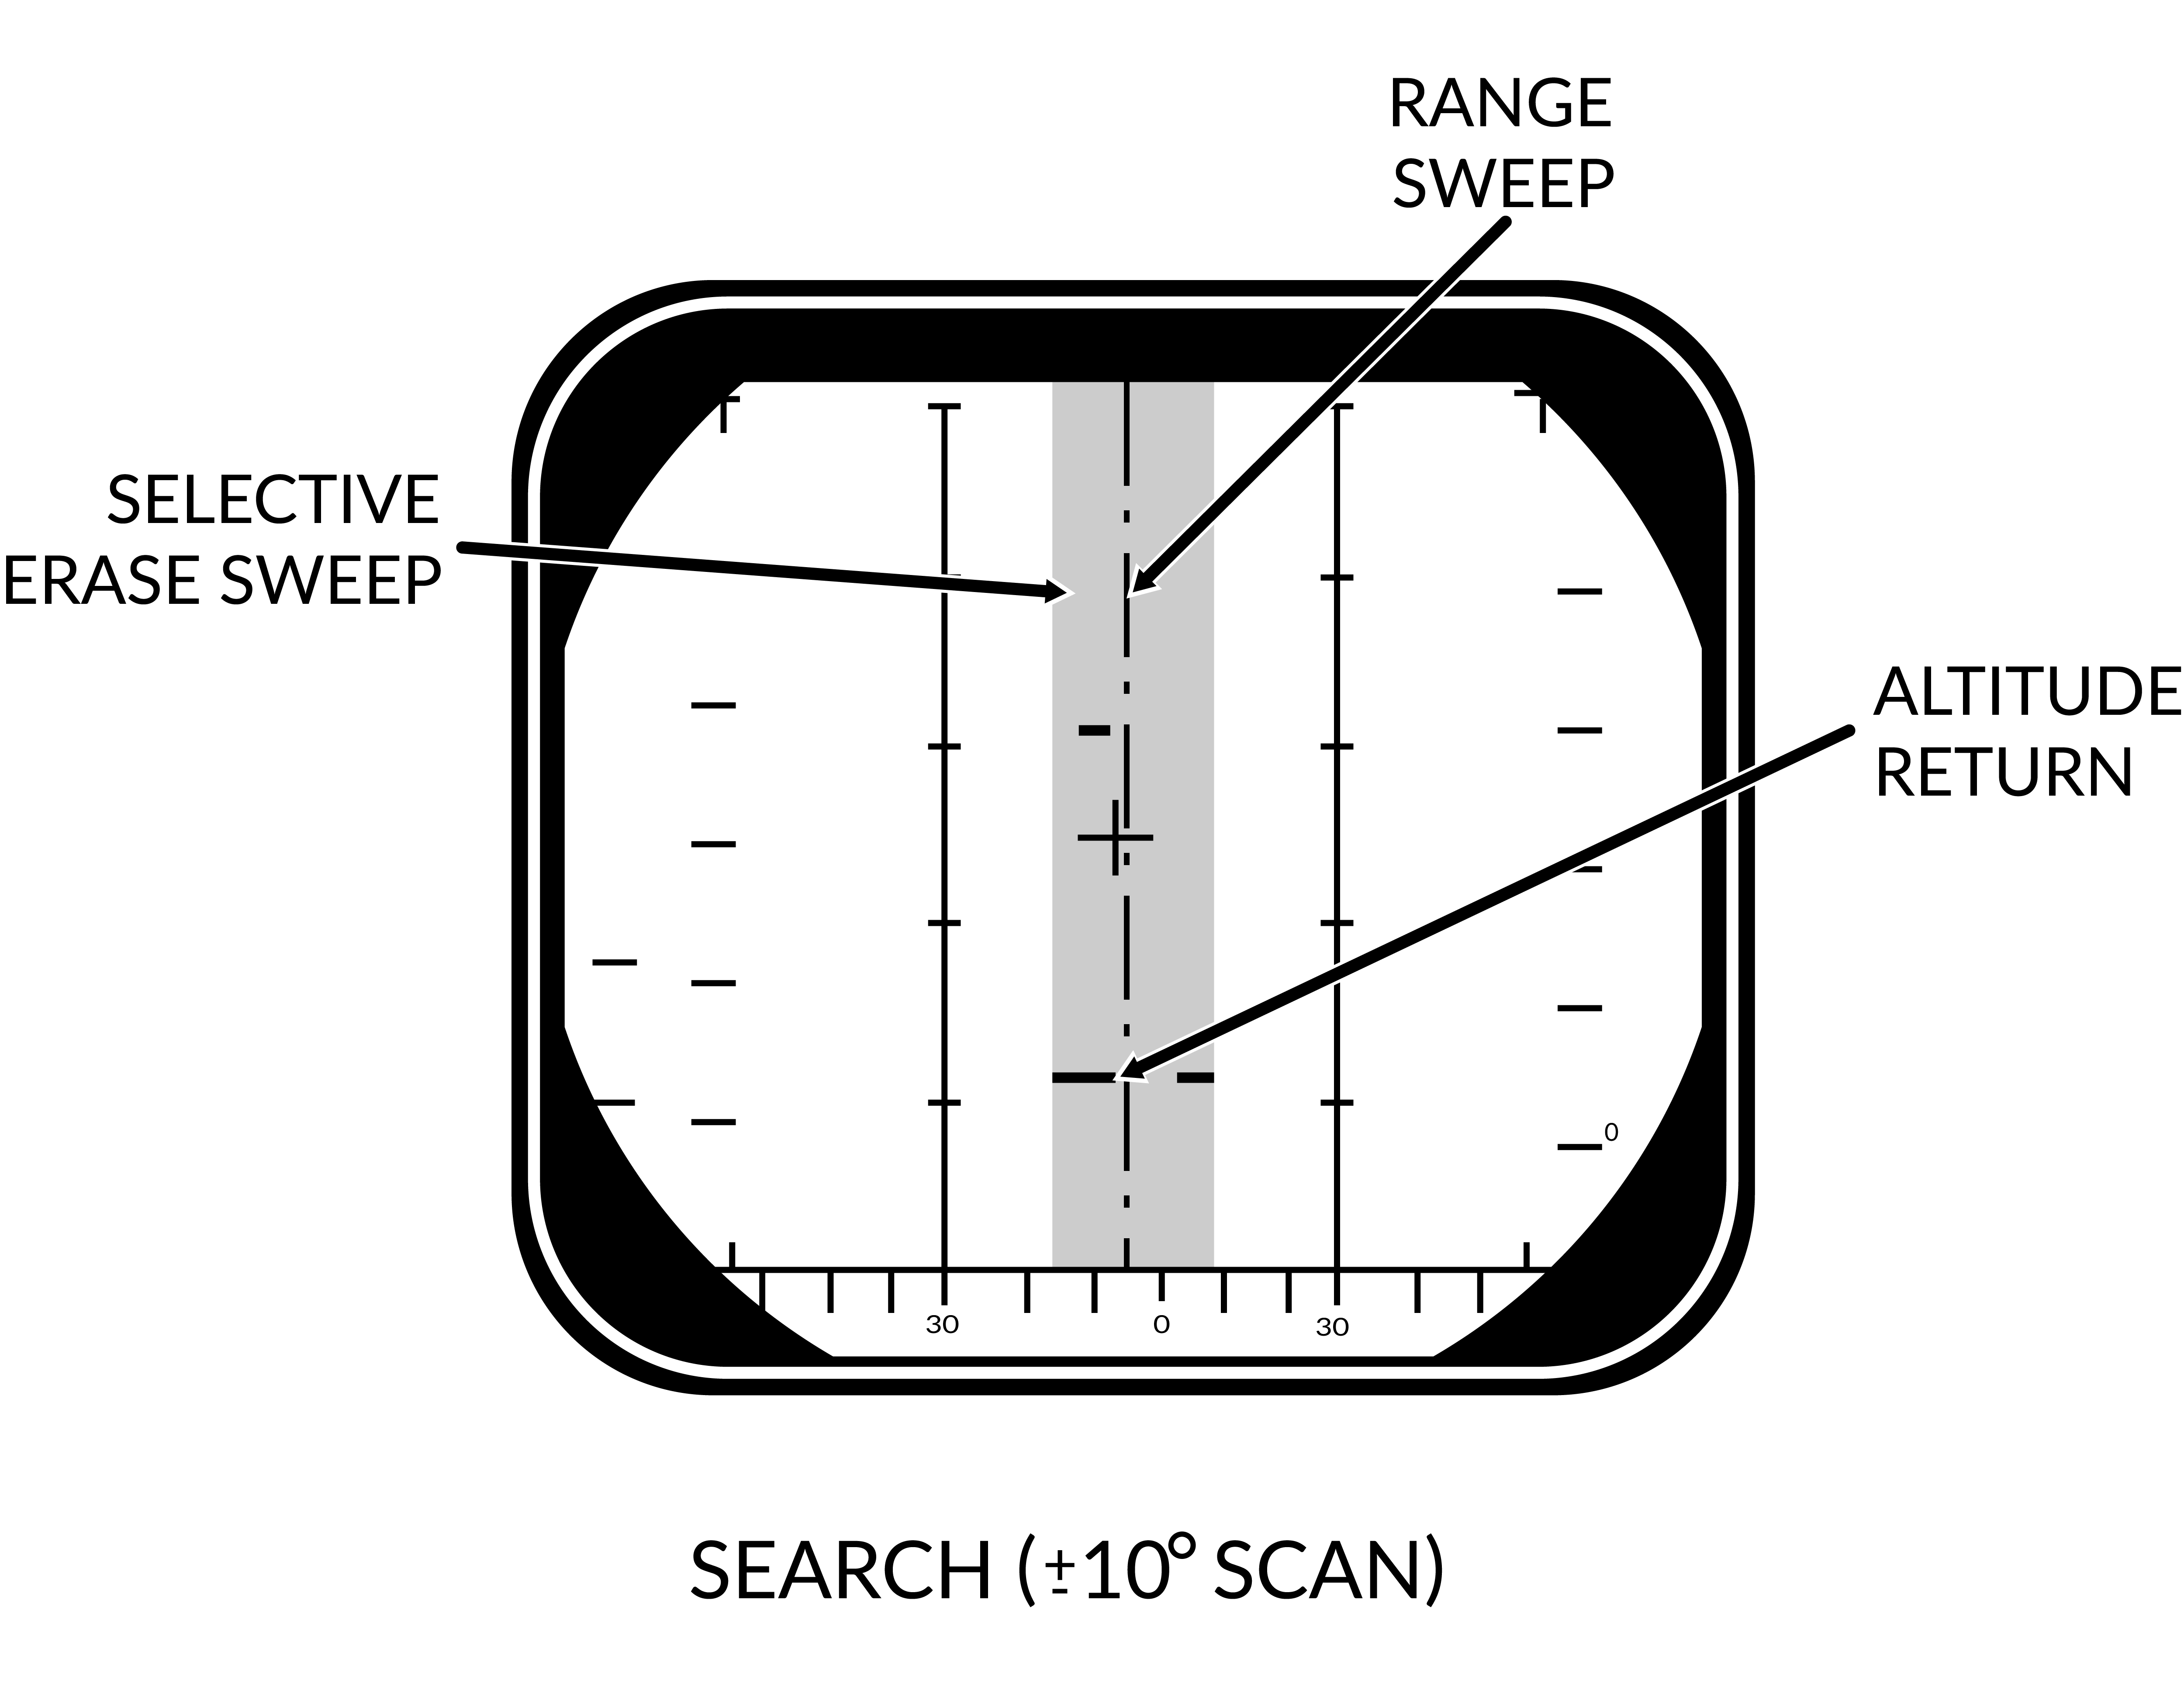
\includegraphics{PSEARCH.png}
			}
		\end{center}
		\begin{center}
			\begin{longtable}{l p{3cm} | p{8cm}}
				\toprule
				\textbullet & \blue{Pulse Search} &  \textbf{Basic Mode} - AWG-9 does not use pulse doppler filtering

				\begin{minipage}[t]{\linewidth}
					\vspace{-7pt}
					\begin{itemize}
						\item \textbf{Advantages}
						\begin{itemize}
							\item All aspect target detection
							\item Cannot be notched
							\item Rudimentary ground mapping
						\end{itemize}
						\item \textbf{Disadvantages}
						\begin{itemize}
							\item Cannot discern ground returns and targets
							\item Lower range
						\end{itemize}
					\end{itemize}
				\end{minipage} \\
				\midrule
				\textbullet & \blue{DDD} &
				\begin{minipage}[t]{\linewidth}
					\vspace{-7pt}
					\begin{itemize}
						\item \textbf{Range/Azimuth}
						\item Visual representation of radar and erase sweeps
					\end{itemize}
				\end{minipage} \\
				\midrule
				\textbullet & \blue{TID} &
				\begin{minipage}[t]{\linewidth}
					\vspace{-7pt}
					\begin{itemize}
						\item \textbf{No Information from Pulse}
						\item \textbf{Cannot guide AIM-54}
					\end{itemize}
				\end{minipage} \\
				\bottomrule
			\end{longtable}
		\end{center}


		\clearpage

		\subsection{PULSE MODE - PSTT}
		\begin{center}
			\resizebox{0.70\linewidth}{!}{
				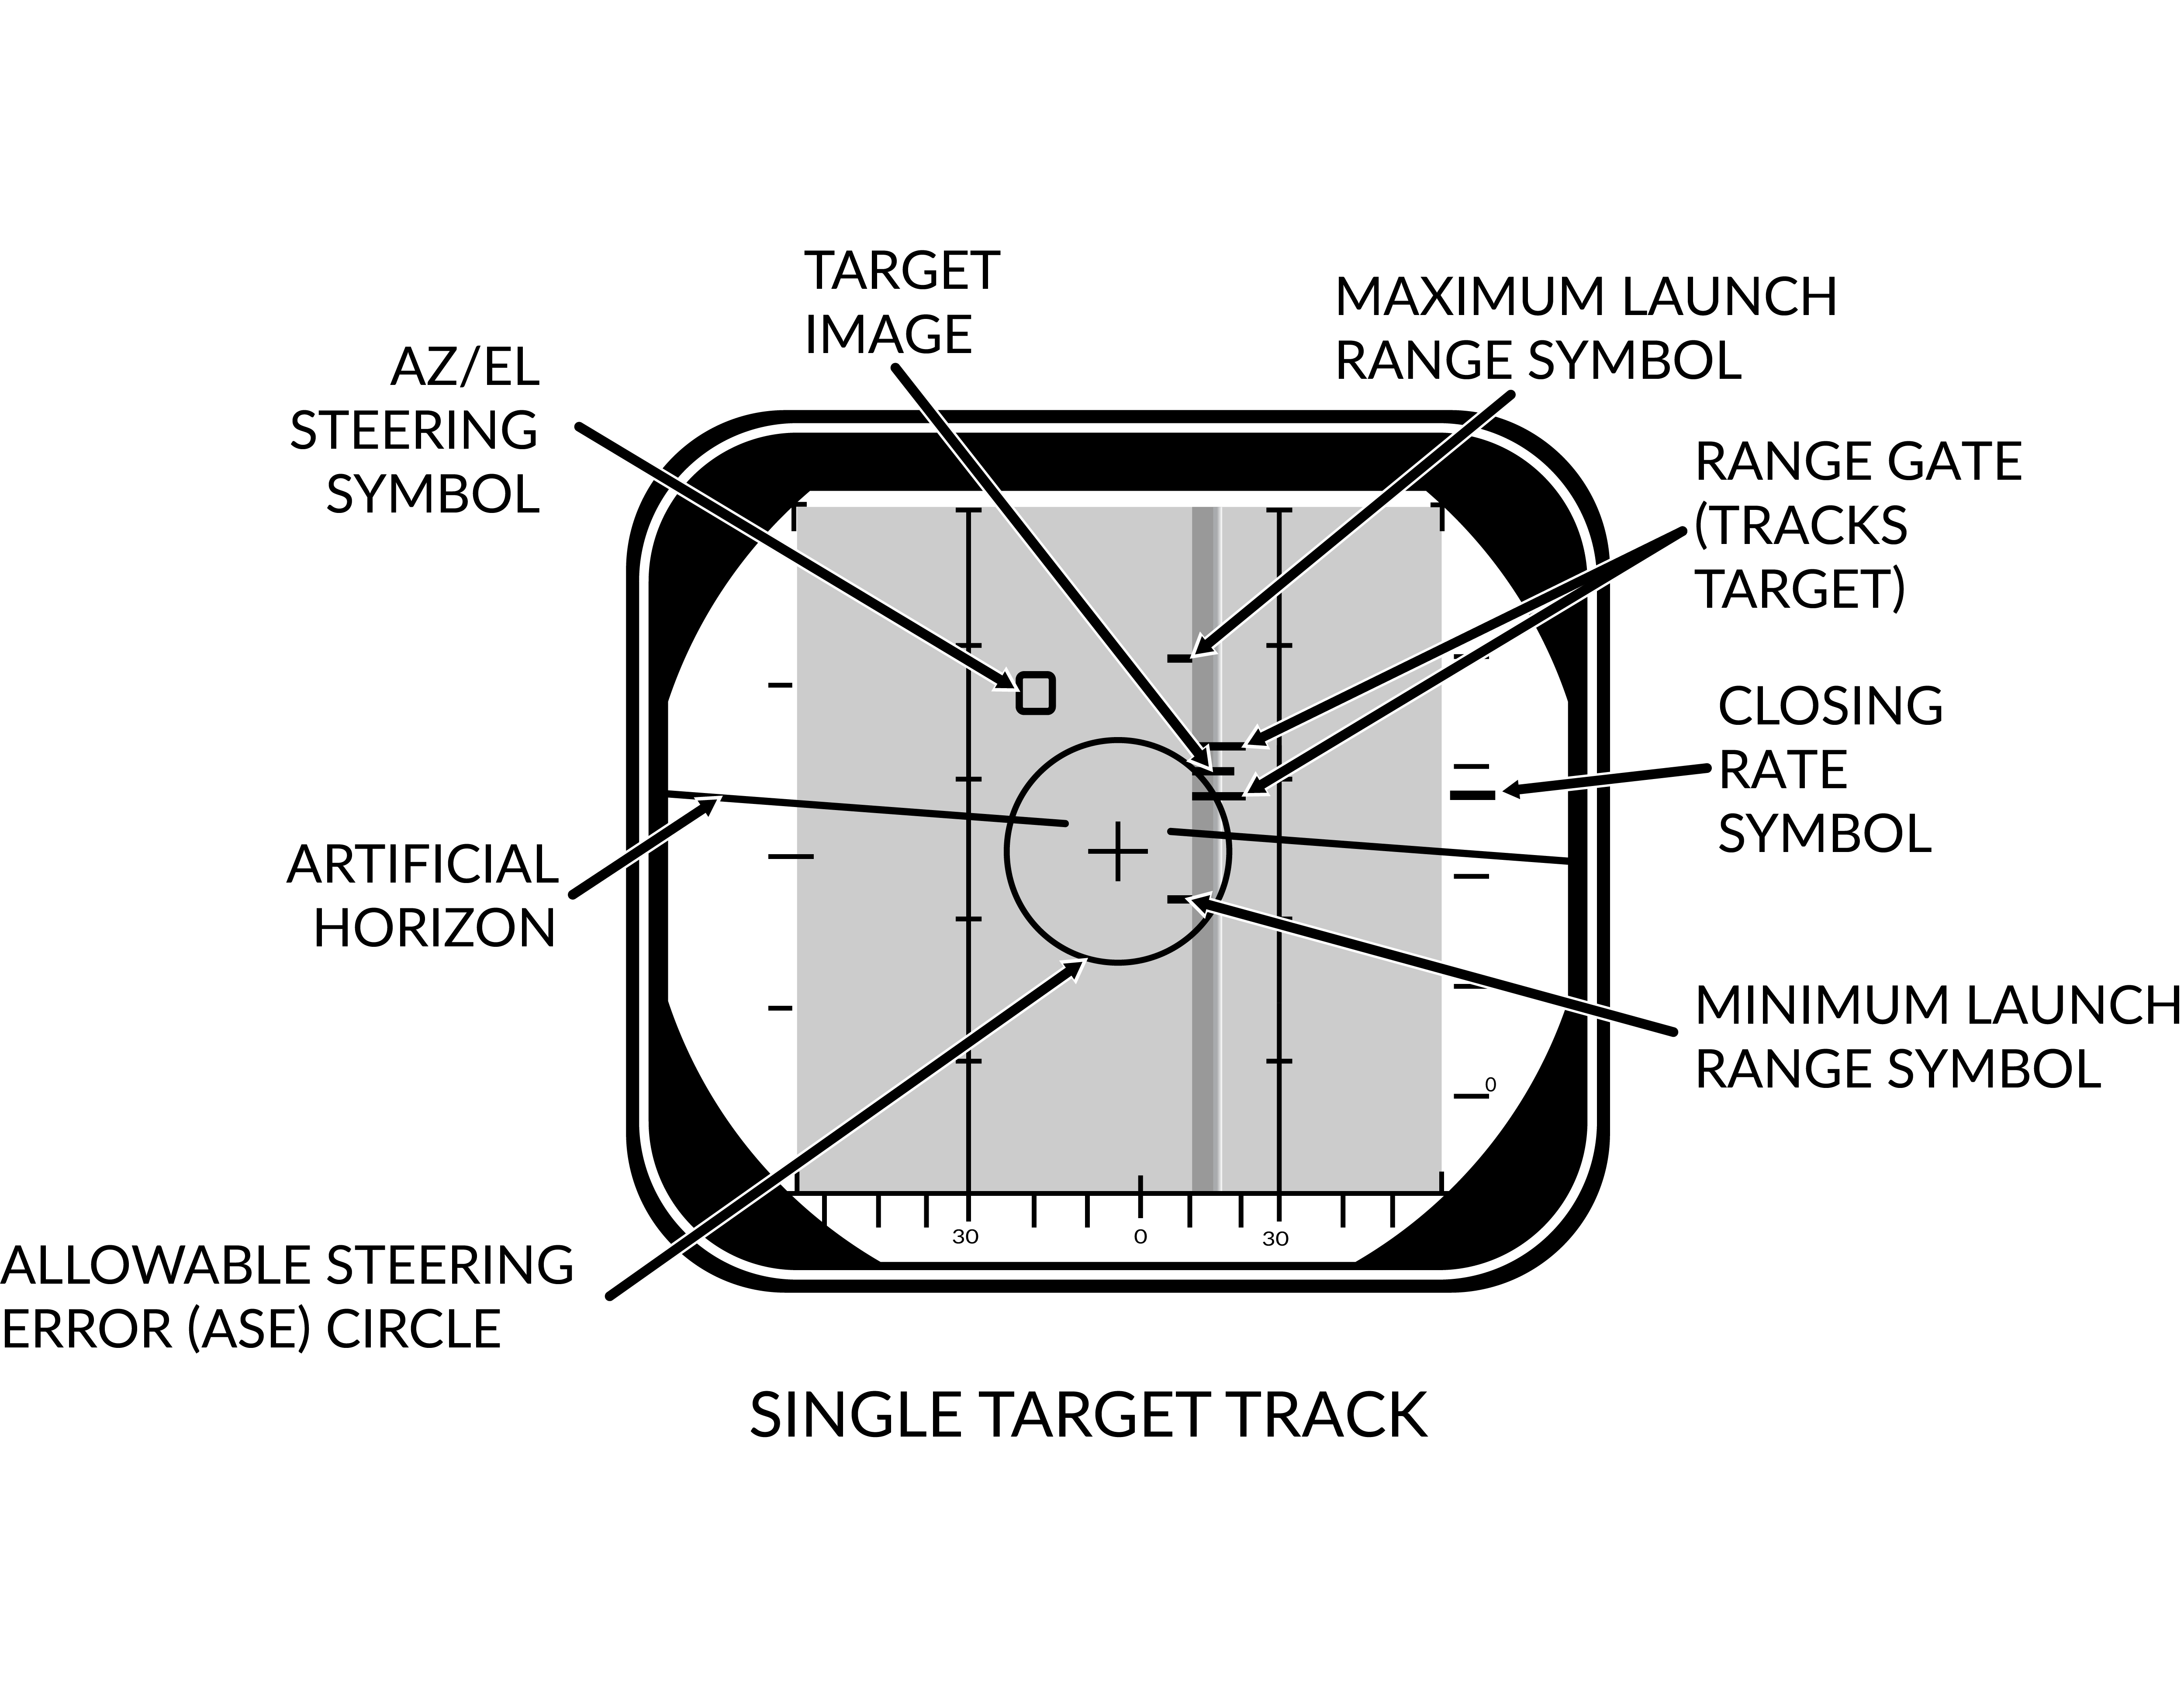
\includegraphics{PSTT.png}
			}
		\end{center}
		\begin{center}
			\begin{longtable}{l p{3cm} | p{8cm}}
				\toprule
				\textbullet & \blue{Pulse STT} &  Lock Target w/o doppler filtering \thumbnar

				\begin{minipage}[t]{\linewidth}
					\vspace{-7pt}
					\begin{itemize}
						\item \textbf{Advantages}
						\begin{itemize}
							\item Cannot be notched
						\end{itemize}
						\item \textbf{Disadvantages}
						\begin{itemize}
							\item Susceptible to ground clutter
						\end{itemize}
					\end{itemize}
				\end{minipage} \\
				\midrule
				\textbullet & \blue{Lock Target} &
				\begin{minipage}[t]{\linewidth}
					\vspace{-7pt}
					\begin{itemize}
						\item \textbf{Conditions}
						\begin{itemize}
							\item Pulse Search Mode selected
							\item RDR HCU Mode selected
						\end{itemize}
						\item \textbf{Lock Target}
						\begin{enumerate}[label=(\alph*)]
							\item Hold HCU Half-action
							\item Slew to desired Target
							\item HCU Full-Action to lock
						\end{enumerate}
						\item \textbf{Unlock Target}
						\begin{enumerate}[label=(\alph*), resume]
							\item HCU Half-action
						\end{enumerate}
					\end{itemize}
				\end{minipage} \\
				\midrule
				\textbullet & \blue{DDD} &
				\begin{minipage}[t]{\linewidth}
					\vspace{-7pt}
					\begin{itemize}
						\item \textbf{Track Indications}
						\begin{itemize}
							\item ANT TRK light
							\item RDROT light
							\item Tracking gates
							\item Closure rate
							\item Attack Symbology
						\end{itemize}
					\end{itemize}
				\end{minipage} \\
				\bottomrule
			\end{longtable}
		\end{center}

		\clearpage

		\subsection{PULSE DOPPLER MODE - PULSE DOPPLER SEARCH}
		\begin{center}
			\resizebox{0.70\linewidth}{!}{
				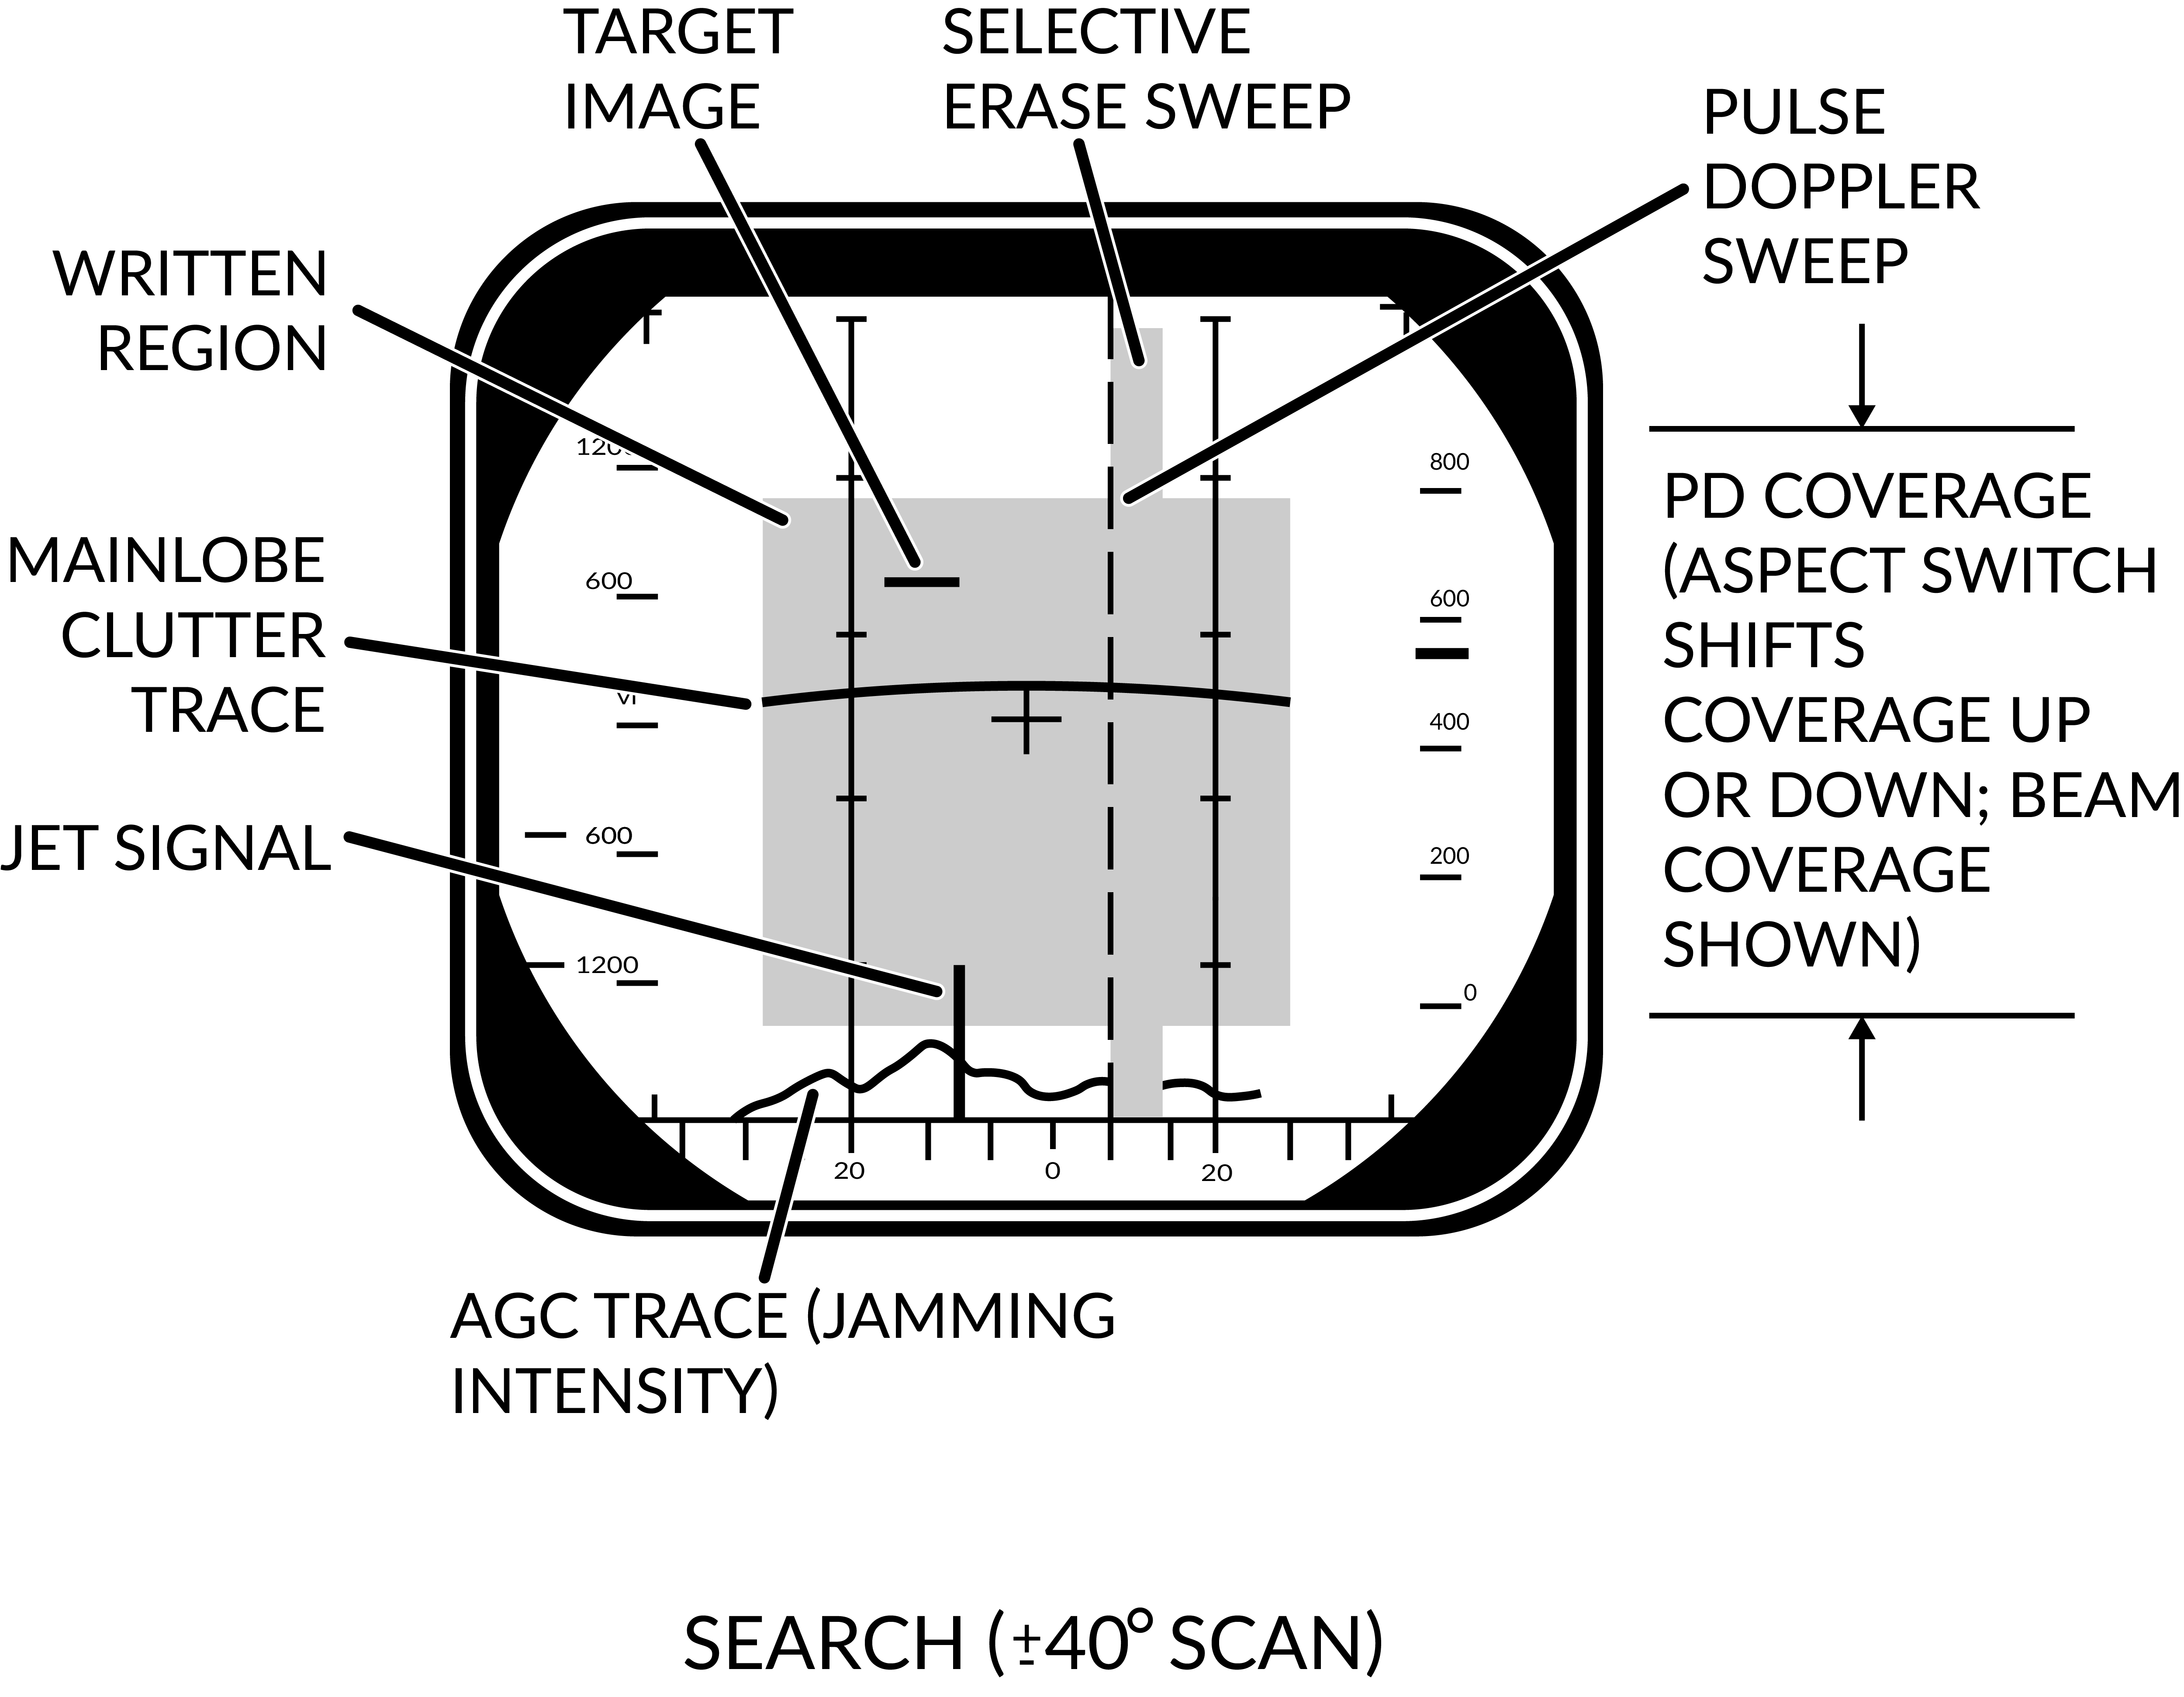
\includegraphics{PDSEARCH.png}
			}
		\end{center}
		\begin{center}
			\begin{longtable}{l p{3cm} | p{8cm}}
				\toprule
				\textbullet & \blue{Pulse Doppler Search} & \textbf{``Early Warning'' Mode} - Longest Range, cannot display range

				\begin{minipage}[t]{\linewidth}
					\vspace{-7pt}
					\begin{itemize}
						\item \textbf{Advantages}
						\begin{itemize}
							\item Longest Range
							\item Doppler Filtering
							\item \textbf{``Look Down Shoot Down''}
						\end{itemize}
						\item \textbf{Disadvantages}
						\begin{itemize}
							\item Can be notched
							\item No range information
						\end{itemize}
					\end{itemize}
				\end{minipage} \\
				\midrule
				\textbullet & \blue{DDD} &
				\begin{minipage}[t]{\linewidth}
					\vspace{-7pt}
					\begin{itemize}
						\item \textbf{Closure Rate/Azimuth}
						\item Visual representation of radar and erase sweeps
					\end{itemize}
				\end{minipage} \\
				\midrule
				\textbullet & \blue{Doppler Filters} &
				\begin{minipage}[t]{\linewidth}
					\vspace{-7pt}
					\begin{itemize}
						\item \textbf{Main Lobe Clutter (MLC) Filter}
						\begin{itemize}
							\item \textbf{Own GS +/- 133 knots}
							\item Removes main ground return
							\item Source of notching
						\end{itemize}
						\item \textbf{Zero Doppler Filter}
						\begin{itemize}
							\item \textbf{Negative own GS +/- 100 knots}
							\item Removes Radar reflection from ground directly beneath own AC
						\end{itemize}
					\end{itemize}
				\end{minipage} \\
				\midrule
				\textbullet & \dblue{MLC Switch} &
				\begin{minipage}[t]{\linewidth}
					\vspace{-7pt}
					\begin{itemize}
						\item \textbf{IN:} Enables MLC filter
						\item \textbf{AUTO:} Enables MLC filter if look-up angle less than 3 deg
						\item \textbf{OUT:} Disables MLC filter
					\end{itemize}
				\end{minipage} \\
				\midrule
				\textbullet & \dblue{Vc Switch} & Changes closure rate DDD scale

				\begin{minipage}[t]{\linewidth}
					\vspace{-7pt}
					\begin{itemize}
						\item \textbf{X-4:} -800 to 4000 knots
						\item \textbf{NORM:} -200 to 1000 knots
						\item \textbf{VID:} -50 to 250 knots
					\end{itemize}
				\end{minipage} \\
				\midrule
				\textbullet & \blue{ASPECT Switch} & Changes closure rate processing scale

				\begin{minipage}[t]{\linewidth}
					\vspace{-7pt}
					\begin{itemize}
						\item \textbf{NOSE:} -600 to 1800 knots
						\item \textbf{BEAM:} -1200 to 1200 knots
						\item \textbf{TAIL:} -1800 to 600 knots
					\end{itemize}
				\end{minipage} \\
				\bottomrule
			\end{longtable}
		\end{center}
		\begin{center}
			\resizebox{0.40\linewidth}{!}{
				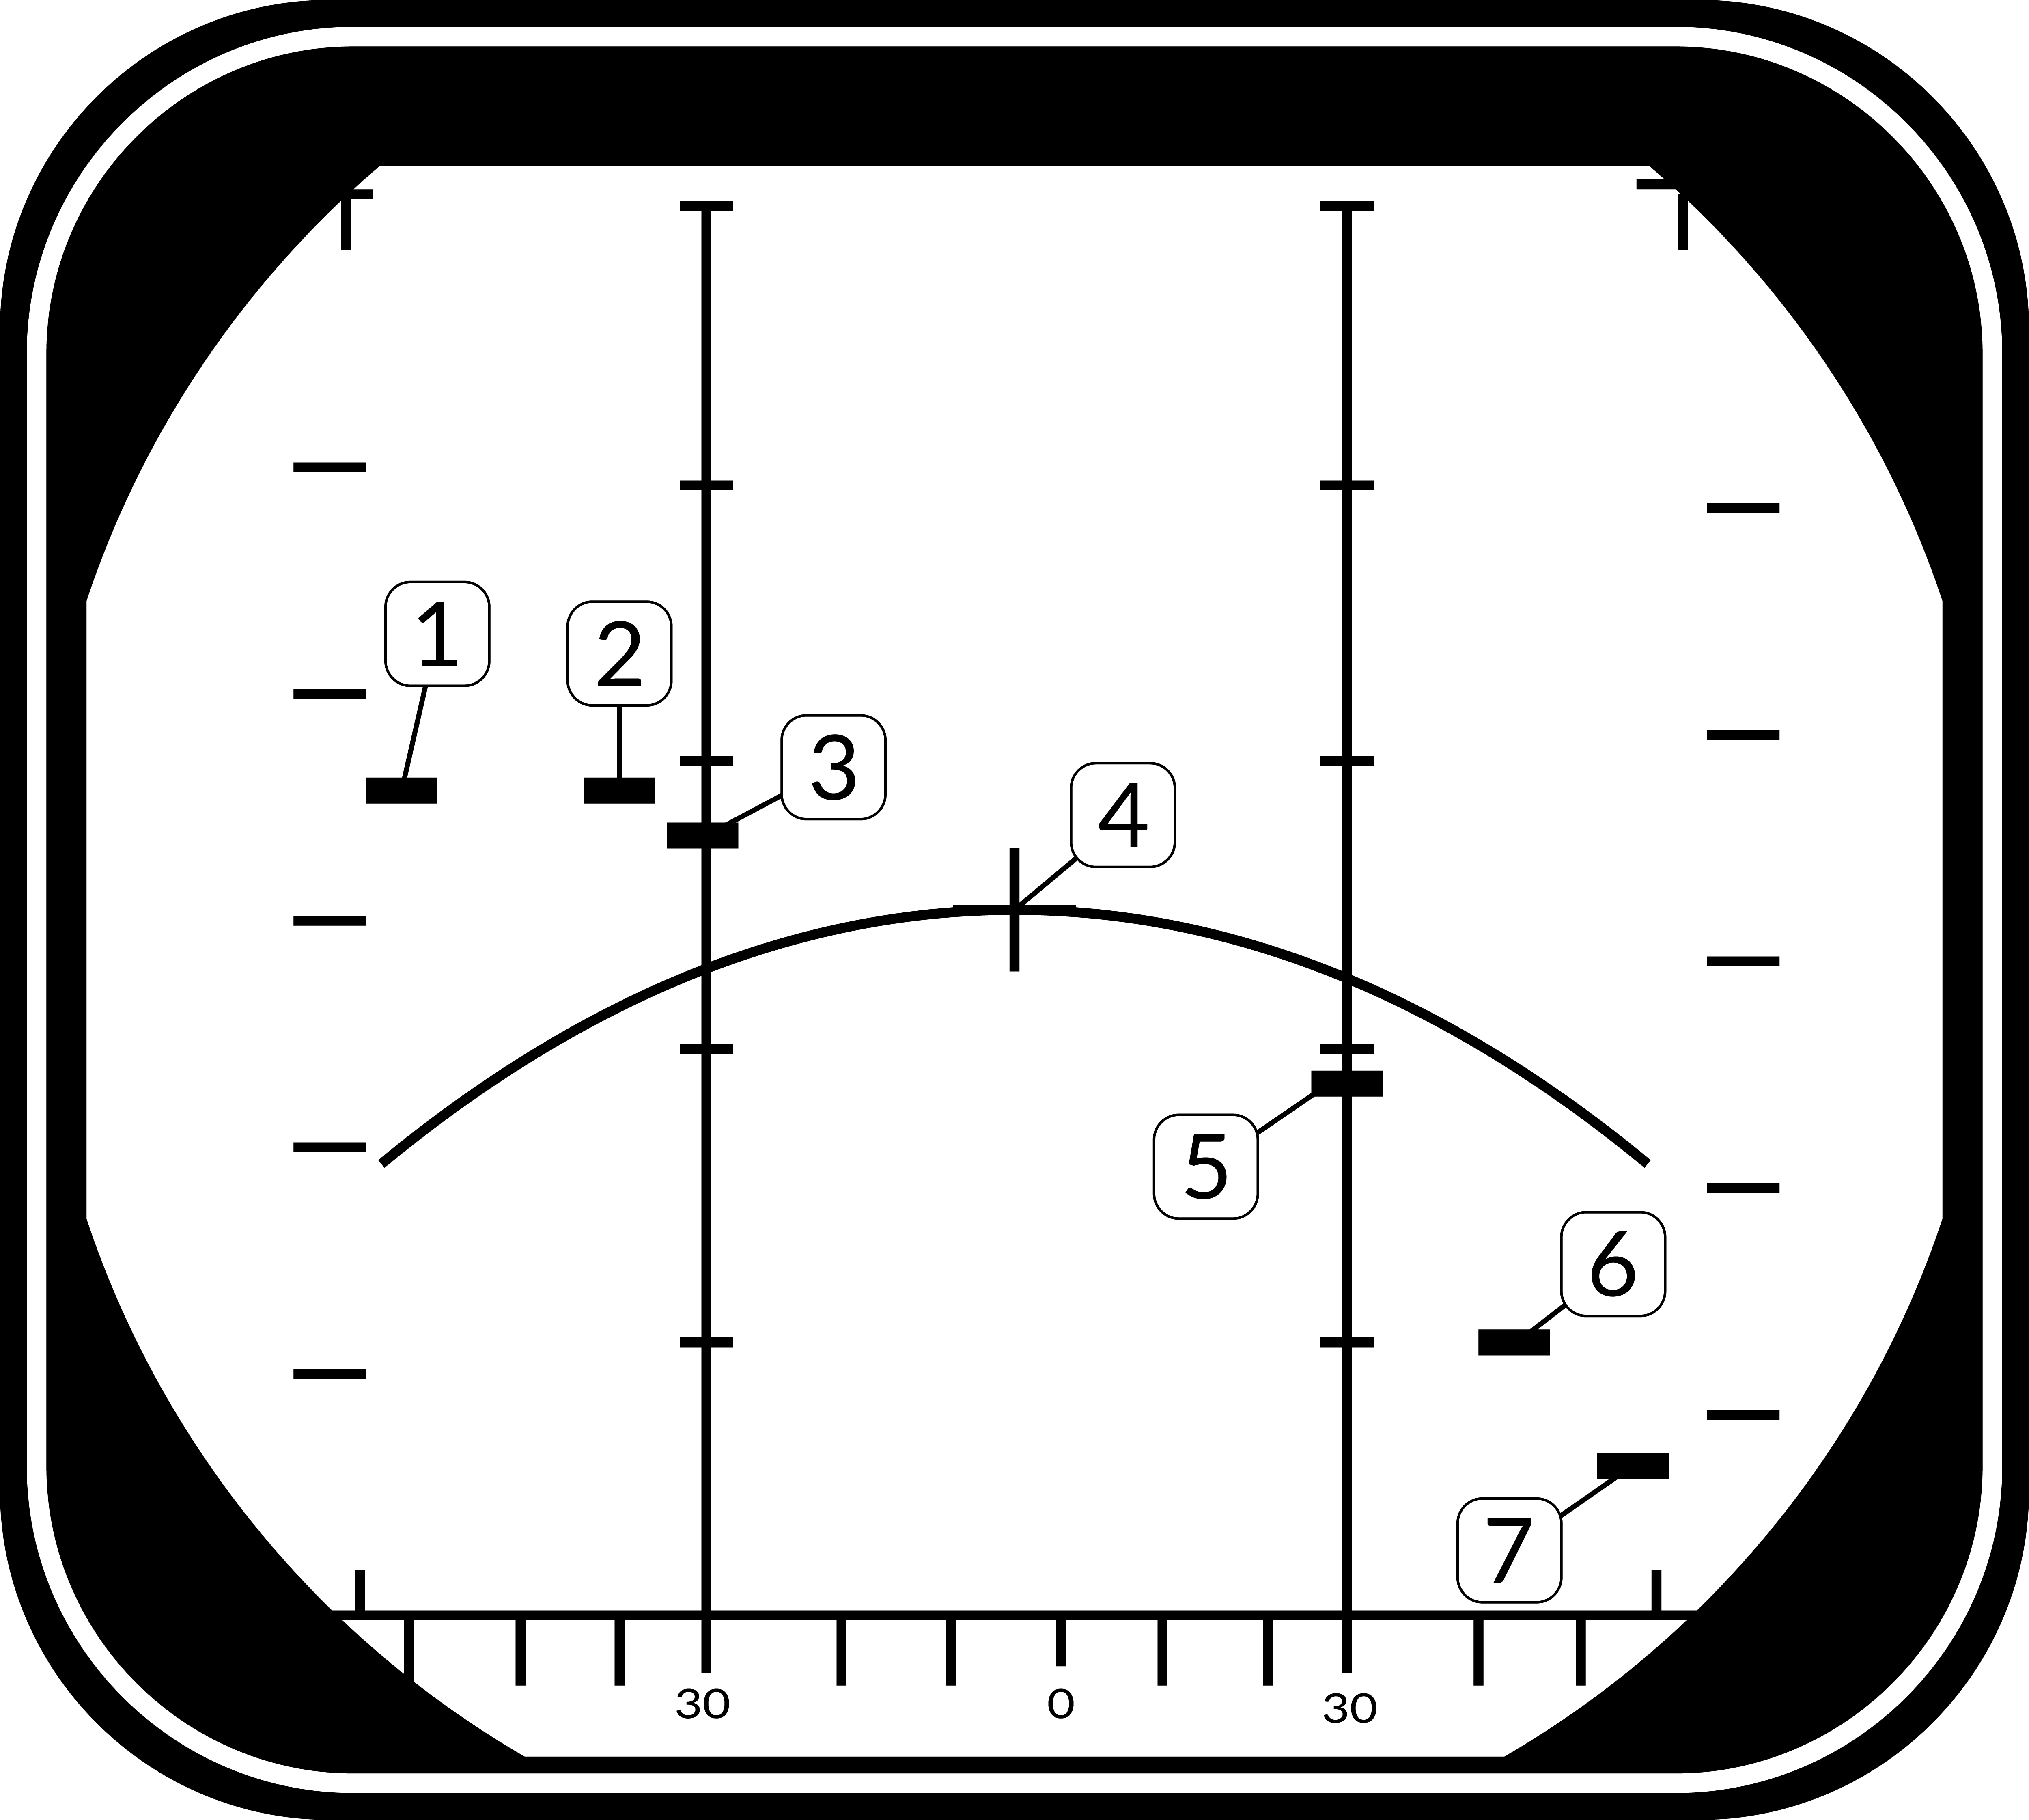
\includegraphics{PD.png}
			}
		\end{center}
		\begin{center}
			\begin{longtable}{l | l | l | l}
				\toprule
				& \blue{Look Angle} & \blue{Line of Sight Rate} & \blue{Target Heading} \\
				\midrule
				\textbf{1} & 60 deg & 1490 & 180 deg \\
				\midrule
				\textbf{2} & 45 deg & 1500 & 120 deg \\
				\midrule
				\textbf{3} & 30 deg & 1428 & 100 deg \\
				\midrule
				\textbf{4} & 0 deg & 1200 & 90 deg \\
				\midrule
				\textbf{5} & 30 deg & 672 & 80 deg \\
				\midrule
				\textbf{6} & 45 deg & 210 & 60 deg \\
				\midrule
				\textbf{7} & 60 deg & -300 & 0 deg \\
				\bottomrule
			\end{longtable}
		\end{center}
		\thumbnar
		\clearpage


		\subsection{PULSE DOPPLER MODE - RWS}
		\label{sec:awg9-rws}
		\begin{center}
			\begin{longtable}{l p{3cm} | p{8cm}}
				\toprule
				\textbullet & \blue{Range While Search} & \textbf{FM Ranging}, used for getting good A/A picture before selecting TWS

				\begin{minipage}[t]{\linewidth}
					\vspace{-7pt}
					\begin{itemize}
						\item \textbf{FM Ranging}
						\begin{itemize}
							\item Pulse Doppler with ranging
							\item TID shows momentary tracks with ranges
							\item Processing reduces max range
						\end{itemize}
						\item \textbf{Advantages}
						\begin{itemize}
							\item Long Range
							\item Doppler Filtering
							\item \textbf{``Look Down Shoot Down''}
							\item Signal Processing
						\end{itemize}
						\item \textbf{Disadvantages}
						\begin{itemize}
							\item Can be notched
						\end{itemize}
					\end{itemize}
				\end{minipage} \\
				\midrule
				\textbullet & \blue{DDD} &
				\begin{minipage}[t]{\linewidth}
					\vspace{-7pt}
					\begin{itemize}
						\item \textbf{Closure Rate/Azimuth}
						\item Visual representation of radar and erase sweeps
					\end{itemize}
				\end{minipage} \\
				\midrule
				\textbullet & \blue{TID} &
				\begin{minipage}[t]{\linewidth}
					\vspace{-7pt}
					\begin{itemize}
						\item \textbf{Momentary Tracks}
						\item Max concurrent tracks: 48
						\item \textbf{Cannot lock targets from TID}
					\end{itemize}
				\end{minipage} \\
				\midrule
				\textbullet & \blue{Filtering} & \textbf{Same as Pulse Doppler Search} \\
				\bottomrule
			\end{longtable}
		\end{center}

		\clearpage

		\subsection{PULSE DOPPLER MODE - TWS}
		\label{sec:awg9-tws}
		\thumbnar
		\begin{center}
			\begin{longtable}{l p{3cm} | p{8cm}}
				\toprule
				\textbullet & \blue{Track While Scan} & \textbf{Builds Track Files}, high situational awareness, multi-target AIM-54 launch

				\begin{minipage}[t]{\linewidth}
					\vspace{-7pt}
					\begin{itemize}
						\item \textbf{Track Files}
						\begin{itemize}
							\item AWG-9 builds Trackfiles for contacts
							\item Can launch multiple AIM-54
							\item Processing reduces max range
							\item Can lock targets from TID
						\end{itemize}
						\item \textbf{FM Ranging}
						\begin{itemize}
							\item Pulse Doppler with ranging
							\item TID shows momentary tracks with ranges
							\item Processing reduces max range
						\end{itemize}
						\item \textbf{Advantages}
						\begin{itemize}
							\item Doppler Filtering
							\item \textbf{Multi-Target AIM-54}
						\end{itemize}
						\item \textbf{Disadvantages}
						\begin{itemize}
							\item \textbf{Lowest Range}
							\item Can be notched
						\end{itemize}
					\end{itemize}
				\end{minipage} \\
				\midrule
				\textbullet & \blue{DDD} &
				\begin{minipage}[t]{\linewidth}
					\vspace{-7pt}
					\begin{itemize}
						\item \textbf{Closure Rate/Azimuth}
						\item Visual representation of radar and erase sweeps
					\end{itemize}
				\end{minipage} \\
				\midrule
				\textbullet & \blue{TID} &
				\begin{minipage}[t]{\linewidth}
					\vspace{-7pt}
					\begin{itemize}
						\item \textbf{Tracksfiles}
						\item Max concurrent tracks: 24
						\item Max displayed tracks: 18
					\end{itemize}
				\end{minipage} \\
				\midrule
				\textbullet & \blue{Filtering} & \textbf{Same as Pulse Doppler Search} \\
				\midrule
				\textbullet & \blue{Scan Volume} & Trackfiles require update every 2.5 s -->
				\begin{minipage}[t]{\linewidth}
					\vspace{-7pt}
					\begin{itemize}
						\item 20 deg 4 bar (if selected)
						\item 40 deg 2 bar (else)
					\end{itemize}
				\end{minipage} \\
				\midrule
				\textbullet & \dblue{TID Mode} \dblue{Selector} &
				\begin{minipage}[t]{\linewidth}
					\vspace{-7pt}
					\begin{itemize}
						\item \textbf{GND STAB:} Ground Stabilized, True North is up on TID
						\item \textbf{A/C STAB:} Aircraft Stabilized
						\item \textbf{ATTAK:} same as A/C STAB with superimposed attack steering symbology
						\item \textbf{TV:} Displays TCS on TID, dispays LANTIRN on TID if equipped
					\end{itemize}
				\end{minipage} \\
				\midrule
				\textbullet & \dblue{TID Display} \dblue{Selector} \dblue{Buttons} &
				\begin{minipage}[t]{\linewidth}
					\vspace{-7pt}
					\begin{itemize}
						\item \textbf{RID DISABLE:} Not simulated
						\item \textbf{ALT NUM:} Enables display of track altitudes on left side of track symbols
						\item \textbf{SYM ELEM:} Enables display of all supplementary symbology of tracks and waypoints
						\item \textbf{DATA LINK:} Enables display of D/L contacts
						\item \textbf{JAM STROBE:} Enables display of jam strobes
						\item \textbf{NON-ATTK:} enables/disables display of targets not possible to engage (friendlies)
						\item \textbf{LAUNCH ZONE:} Enables display of weapon launch zones
						\item \textbf{VEL VECTOR:} Enables display of velocity vectors
					\end{itemize}
				\end{minipage} \\
				\midrule
				\textbullet & \dblue{TRACK HOLD} \dblue{CLSN Steering} \dblue{Buttons} &
				\begin{minipage}[t]{\linewidth}
					\vspace{-7pt}
					\begin{itemize}
						\item \textbf{TRACK HOLD}
						\begin{itemize}
							\item Normally: Tracks maintained for 14 s after last observation
							\item Track Hold: maintained for 2 min after last observation
						\end{itemize}
						\item \textbf{CLSN Button}
						\begin{itemize}
							\item begins collision steering to currently tracked target
							\item enables Steering Centroid if in TWS
							\item LD CLSN presents azimuth steering only
							\item CLSN presents both azimuth and elevation steering
						\end{itemize}
					\end{itemize}
				\end{minipage} \\
				\midrule
				\textbullet & \blue{TWS AUTO / MAN} &
				\begin{minipage}[t]{\linewidth}
					\vspace{-7pt}
					\begin{itemize}
						\item \textbf{TWS MAN:} Manual azimuth/elevation control, target designation by RIO
						\item \textbf{TWS AUTO:} Automatic prioritization of targets and azimuth elevation control
					\end{itemize}
				\end{minipage} \\
				\bottomrule
			\end{longtable}
		\end{center}

		\clearpage

		\subsection{PULSE DOPPLER MODE - TWS MAN}
		\thumbnar
		\begin{center}
			\begin{longtable}{l p{3cm} | p{8cm}}
				\toprule
				\textbullet & \blue{TWS MAN} &
				\begin{minipage}[t]{\linewidth}
					\vspace{-7pt}
					\begin{itemize}
						\item \textbf{Target Selection:} Manual
						\item \textbf{Scan Azimuth/Elevation:} Manual
					\end{itemize}
				\end{minipage} \\
				\midrule
				\textbullet & \blue{Target Selection} &
				\begin{minipage}[t]{\linewidth}
					\vspace{-7pt}
					\begin{itemize}
						\item \textbf{Conditions}
						\begin{itemize}
							\item TWS MAN Radar Mode selected
							\item TID CURSOR TID Mode selected
						\end{itemize}
						\item \textbf{Hook Target}
						\begin{enumerate}[label=(\alph*)]
							\item Hold HCU Half-Action
							\item Slew TID Cursor over desired Tgt
							\item HCU Full-Action to select Tgt
						\end{enumerate}
						\item \textbf{TID Symbology}
						\begin{itemize}
							\item Range (\textbf{RA})
							\item Bearing (\textbf{BR})
							\item Altitude (\textbf{AL})
							\item Magnetic course (\textbf{MC})
						\end{itemize}
						\item \textbf{Lock Target}
						\begin{enumerate}[label=(\alph*), resume]
							\item Press \textbf{PD STT} or \textbf{Pulse STT} buttons
						\end{enumerate}
						\item \textbf{Deselect Target}
						\begin{enumerate}[label=(\alph*), resume]
							\item press HCU Half-Action
						\end{enumerate}
					\end{itemize}
				\end{minipage} \\
				\midrule
				\textbullet & \blue{AIM-54 Launch} &
				\begin{minipage}[t]{\linewidth}
					\vspace{-7pt}
					\begin{itemize}
						\item \textbf{Automatically selects TWS AUTO}
						\item \textbf{Prevents selection of TWS MAN}
					\end{itemize}
				\end{minipage} \\
				\bottomrule
			\end{longtable}
		\end{center}

		\clearpage

		\subsection{PULSE DOPPLER MODE - TWS AUTO}
		\begin{center}
			\begin{longtable}{l p{3cm} | p{8cm}}
				\toprule
				\textbullet & \blue{TWS AUTO} &
				\begin{minipage}[t]{\linewidth}
					\vspace{-7pt}
					\begin{itemize}
						\item \textbf{Target Selection:} prioritizes contacts based off range, aspect, closure
						\item \textbf{Scan Azimuth/Elevation:} Geometric center of targets in scan volume
					\end{itemize}
				\end{minipage} \\
				\midrule
				\textbullet & \blue{Centroid / Steering Cues} &
				\begin{minipage}[t]{\linewidth}
					\vspace{-7pt}
					\begin{itemize}
						\item \textbf{Steering Centroid}
						\begin{itemize}
							\item facilitates steering cues
							\item HUD, VDI, TID, DDD
							\item Appears as \textbf{X} on TID
							\item Takes Gimbal limits into account
							\item Weights individual Tracks based on parameters
						\end{itemize}
						\item \textbf{Illumination Centroid}
						\begin{itemize}
							\item \textbf{Not Visible}
							\item Controls azimuth and elevation of scan pattern
							\item Takes scan volume into account
						\end{itemize}
					\end{itemize}
				\end{minipage} \\
				\midrule
				\textbullet & \blue{Pilot Steering Cues} &
				\begin{minipage}[t]{\linewidth}
					\vspace{-7pt}
					\begin{itemize}
						\item \textbf{Conditions}
						\begin{itemize}
							\item A-A HUD Mode selected
							\item Master Arm ON (UP)
							\item AIM-54 or AIM-7 selected
							\item TWS-AUTO selected
						\end{itemize}
					\end{itemize}
				\end{minipage} \\
				\bottomrule
			\end{longtable}
		\end{center}

		\clearpage

		\subsection{PULSE DOPPLER MODE - PDSTT}
		\begin{center}
			\resizebox{0.70\linewidth}{!}{
				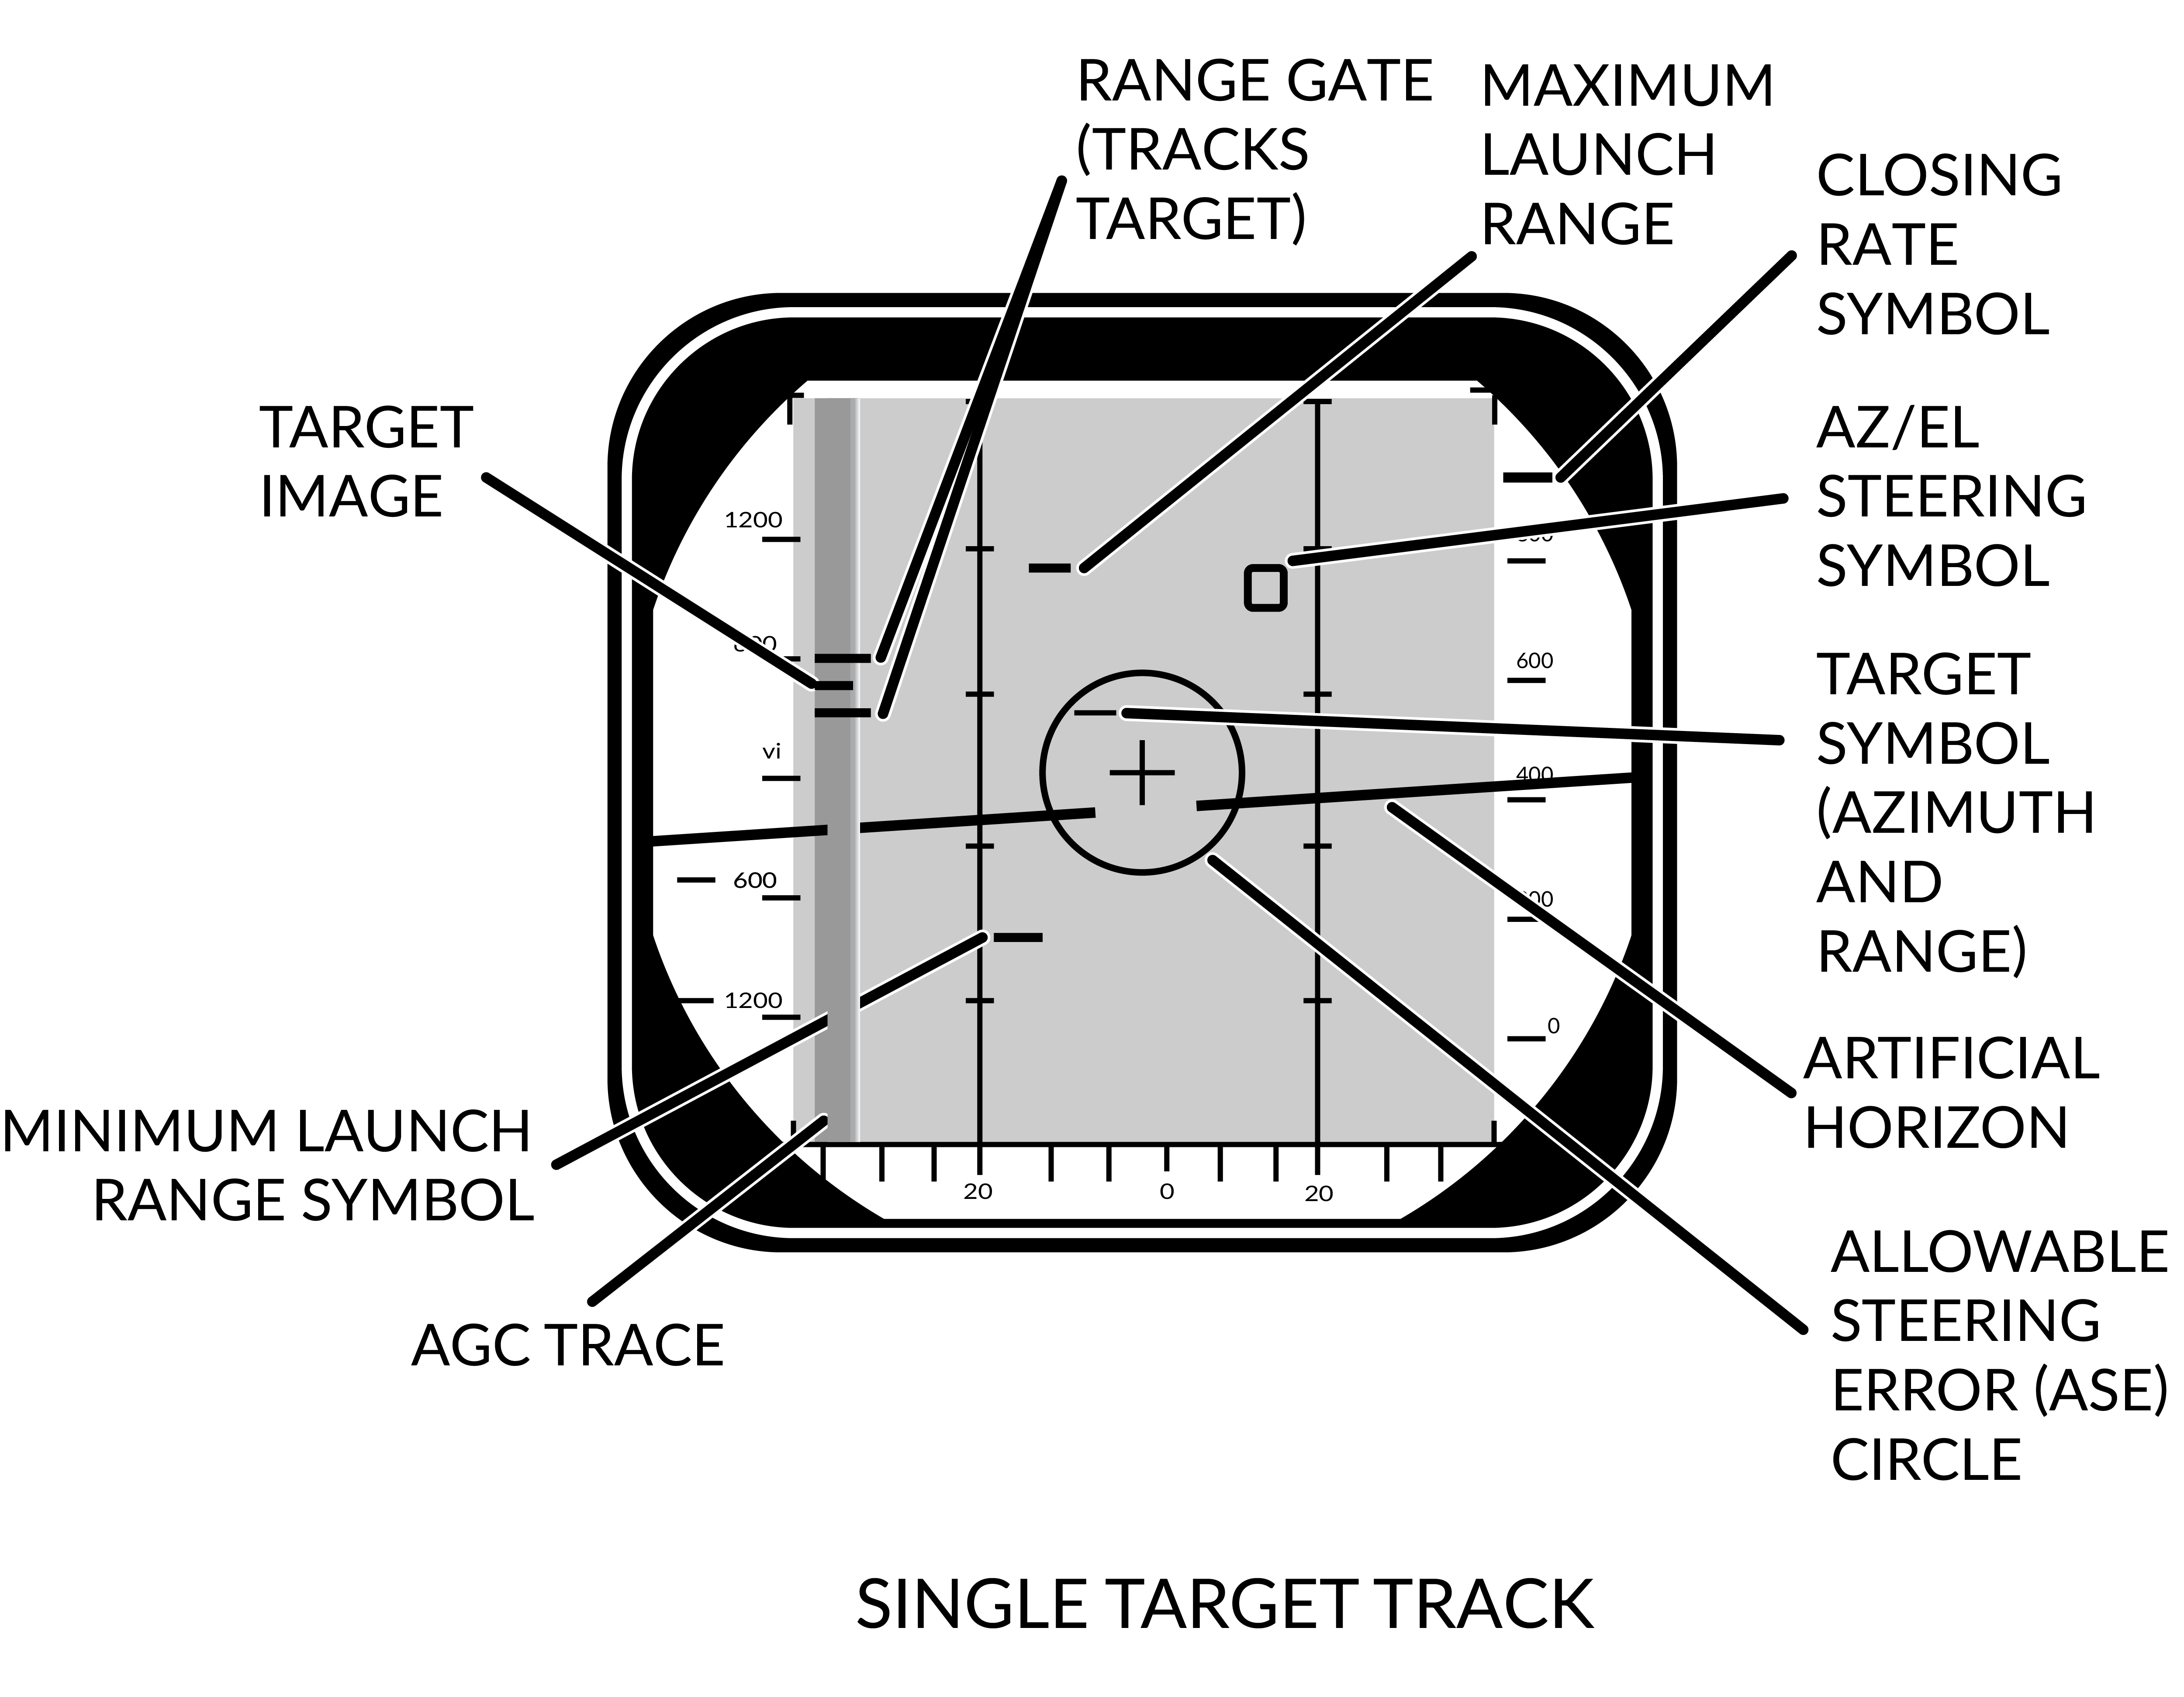
\includegraphics{PDSTT.png}
			}
		\end{center}
		\begin{center}
			\begin{longtable}{l p{3cm} | p{8cm}}
				\toprule
				\textbullet & \blue{Pulse Doppler STT} & Lock Target with doppler filtering \thumbnar
				\begin{minipage}[t]{\linewidth}
					\vspace{-7pt}
					\begin{itemize}
						\item \textbf{Advantages}
						\begin{itemize}
							\item Ground Clutter filtering
						\end{itemize}
						\item \textbf{Disadvantages}
						\begin{itemize}
							\item Susceptible to notching
						\end{itemize}
					\end{itemize}
				\end{minipage} \\
				\midrule
				\textbullet & \blue{Lock Target} &
				\begin{minipage}[t]{\linewidth}
					\vspace{-7pt}
					\begin{itemize}
						\item \textbf{Conditions}
						\begin{itemize}
							\item Pulse Doppler Mode selected (PD Search, RWS, TWS)
							\item RDR HCU Mode selected
						\end{itemize}
						\item \textbf{Lock Target}
						\begin{enumerate}[label=(\alph*)]
							\item Hold HCU Half-action
							\item Slew to desired Target
							\item HCU Full-Action to lock
						\end{enumerate}
						\item \textbf{Unlock Target}
						\begin{enumerate}[label=(\alph*), resume]
							\item HCU Half-action
						\end{enumerate}
					\end{itemize}
				\end{minipage} \\
				\midrule
				\textbullet & \blue{DDD} &
				\begin{minipage}[t]{\linewidth}
					\vspace{-7pt}
					\begin{itemize}
						\item \textbf{Track Indications}
						\begin{itemize}
							\item ANT TRK light
							\item RDROT light
							\item Tracking gates
							\item Closure rate
							\item Attack Symbology
						\end{itemize}
					\end{itemize}
				\end{minipage} \\
				\bottomrule
			\end{longtable}
		\end{center}

		\subsection{ACM MODES - OVERVIEW}
		\begin{center}
			\begin{tabular}{p{3cm} | p{2cm}  | p{2cm} | p{2cm} | p{2cm}}
				\toprule
				& \blue{PLM} & \blue{VSL} & \blue{PAL} & \blue{MRL} \\
				\midrule
				\textbf{Range} & 5 nm & 5 nm & 15 nm & 5 nm \\
				\midrule
				\textbf{Description} & Boresight & Vertical & Horizontal & RIO \\
				\midrule
				\textbf{Weapons} & \multicolumn{4}{c}{Gun + All Missiles} \\
				\bottomrule
			\end{tabular}
		\end{center}
		\begin{center}
			\begin{longtable}{l p{3cm} | p{8cm}}
				\toprule
				\textbullet & \blue{PLM} &
				\begin{minipage}[t]{0.53\linewidth}
					\vspace{-7pt}
					\begin{itemize}
						\item \textbf{Pilot Lockon Mode}
						\item \textbf{Highest Priority ACM}
						\item \textbf{Search Pattern}
						\begin{itemize}
							\item Small Boresight
							\item Range: 5 nm
						\end{itemize}
					\end{itemize}
				\end{minipage}
				\begin{minipage}[t]{0.45\linewidth}
					\vspace{-7pt}
					\centering
					\includegraphics[width=\linewidth]{PLM.png}
				\end{minipage} \\
				\midrule
				\textbullet & \blue{VSL} &
				\begin{minipage}[t]{\linewidth}
					\vspace{-7pt}
					\begin{itemize}
						\item \textbf{Vertical Scan Lockon}
						\item \textbf{HI Search Pattern}
						\begin{itemize}
							\item Width: 5 deg
							\item Vertical: +15 to +55 deg
							\item Range: 5 nm
						\end{itemize}
						\item \textbf{LO Search Pattern}
						\begin{itemize}
							\item Width: 5 deg
							\item Vertical: -15 to +25 deg
							\item Range: 5 nm
						\end{itemize}
						\item \textbf{RIO/PILOT Controlled}
					\end{itemize}
				\end{minipage} \\
				\midrule
				\textbullet & \blue{PAL} &
				\begin{minipage}[t]{\linewidth}
					\vspace{-7pt}
					\begin{itemize}
						\item \textbf{Pilot Automatic Lockon}
						\item \textbf{Search Pattern}
						\begin{itemize}
							\item Width: +/- 20 deg
							\item Vertical: 8-bar
							\item Range: 15 nm
						\end{itemize}
					\end{itemize}
				\end{minipage} \\
				\midrule
				\textbullet & \blue{MRL} &
				\begin{minipage}[t]{\linewidth}
					\vspace{-7pt}
					\begin{itemize}
						\item \textbf{Manual Rapid Lockon}
						\item \textbf{RIO Controlled}
						\item \textbf{Search Pattern}
						\begin{itemize}
							\item HCU Controlled
							\item Range: 5 nm
						\end{itemize}
					\end{itemize}
				\end{minipage} \\
				\bottomrule
			\end{longtable}
		\end{center}

		\subsection{APX-76 IFF}


		\cleardoublepage

		\hypertarget{subsec:tidsymb}{}
		\subsection{TID SYMBOLOGY}
		\begin{center}
			\begin{longtable}{p{3.5cm} | p{1cm} |  p{6cm}}
				\toprule
				\multicolumn{2}{c}{\blue{GENERAL}} & \thumbnar \\
				\midrule
				\textbf{Center Dot} &
				\begin{minipage}[t]{\linewidth}
					\vspace{-7pt}
					\centering
					
\includegraphics[width=0.05cm]{1.png}
				\end{minipage} &
				\begin{minipage}[t]{\linewidth}
					\vspace{-7pt}
					\begin{itemize}
						\item \textbf{Basic Component of Symbols}
						\begin{itemize}
							\item Marks coordinates of symbol
						\end{itemize}
					\end{itemize}
				\end{minipage} \\
				\midrule
				\textbf{Own AC} &
				\begin{minipage}[t]{\linewidth}
					\vspace{-7pt}
					\centering
					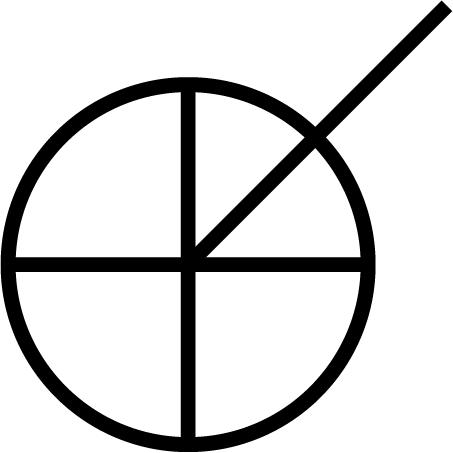
\includegraphics[width=0.8cm]{2.png}
				\end{minipage} &
				\begin{minipage}[t]{\linewidth}
					\vspace{-7pt}
					\begin{itemize}
						\item \textbf{Symbol representing own aircraft}
						\begin{itemize}
							\item Ground Stabilized: Moves
							\item Aircraft Stabilized: Stationary
							\item Outside TID: line drawn from TID center towards symbol
						\end{itemize}
					\end{itemize}
				\end{minipage} \\
				\midrule
				\textbf{TID Cursor} &
				\begin{minipage}[t]{\linewidth}
					\vspace{-7pt}
					\centering
					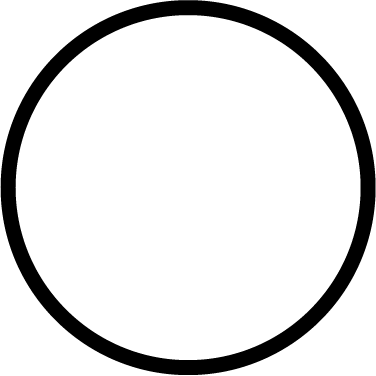
\includegraphics[width=0.8cm]{26.png}
				\end{minipage} &
				\begin{minipage}[t]{\linewidth}
					\vspace{-7pt}
					\begin{itemize}
						\item \textbf{Hook Cursor}
						\begin{itemize}
							\item Controlled by \textbf{HCU} in \textbf{TID mode}
						\end{itemize}
						\item \textbf{Half-Action}
						\begin{itemize}
							\item Enables display of symbol
							\item Enables HCU stick to move cursor
						\end{itemize}
						\item \textbf{Full-Action}
						\begin{itemize}
							\item Hooks closest symbol
							\item If no symbol near, cursor dropped at location
						\end{itemize}
					\end{itemize}
				\end{minipage} \\
				\midrule
				\textbf{TWS Steering Centroid} &
				\begin{minipage}[t]{\linewidth}
					\vspace{-7pt}
					\centering
					
\includegraphics[width=0.8cm]{27.png}
				\end{minipage} &
				\begin{minipage}[t]{\linewidth}
					\vspace{-7pt}
					\begin{itemize}
						\item \textbf{Steering centroid of TWS tracks}
						\begin{itemize}
							\item Selected by WCS for weapons engagement
						\end{itemize}
					\end{itemize}
				\end{minipage} \\
				\midrule
				\multicolumn{2}{c|}{\blue{ONBOARD SENSORS}} & \textbf{Symbol Above Dot} \\
				\midrule
				\textbf{Unknown} &
				\begin{minipage}[t]{\linewidth}
					\vspace{-7pt}
					\centering
					
\includegraphics[width=0.8cm]{3.png}
				\end{minipage} &
				\begin{minipage}[t]{\linewidth}
					\vspace{-7pt}
					\begin{itemize}
						\item \textbf{Unknown Sensor Track}
						\item \textbf{All Returns in RWS}
					\end{itemize}
				\end{minipage} \\
				\midrule
				\textbf{Hostile} &
				\begin{minipage}[t]{\linewidth}
					\vspace{-7pt}
					\centering
					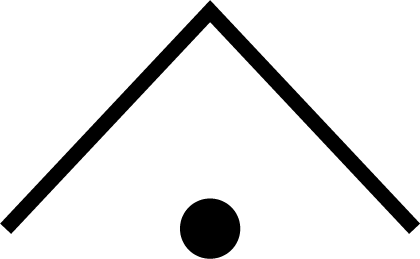
\includegraphics[width=0.8cm]{4.png}
				\end{minipage} &
				\begin{minipage}[t]{\linewidth}
					\vspace{-7pt}
					\begin{itemize}
						\item \textbf{Sensor Track designated Hostile by RIO}
					\end{itemize}
				\end{minipage} \\
				\midrule
				\textbf{Friend} &
				\begin{minipage}[t]{\linewidth}
					\vspace{-7pt}
					\centering
					
\includegraphics[width=0.8cm]{5.png}
				\end{minipage} &
				\begin{minipage}[t]{\linewidth}
					\vspace{-7pt}
					\begin{itemize}
						\item \textbf{Sensor Track designated Friendly by RIO}
					\end{itemize}
				\end{minipage} \\
				\midrule
				\textbf{Angle-Tracked Radar Target} &
				\begin{minipage}[t]{\linewidth}
					\vspace{-7pt}
					\centering
					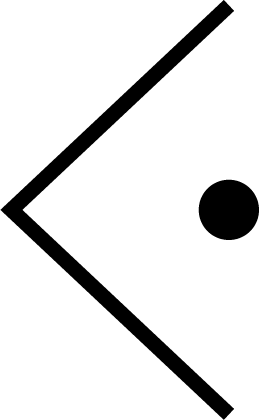
\includegraphics[width=0.55cm]{6.png}
				\end{minipage} &
				\begin{minipage}[t]{\linewidth}
					\vspace{-7pt}
					\begin{itemize}
						\item \textbf{Radar Angle Tracking}
						\begin{itemize}
							\item Jamming Target
						\end{itemize}
					\end{itemize}
				\end{minipage} \\
				\midrule
				\textbf{Angle-Tracked Radar Target with Altitude Difference Ranging} &
				\begin{minipage}[t]{\linewidth}
					\vspace{-7pt}
					\centering
					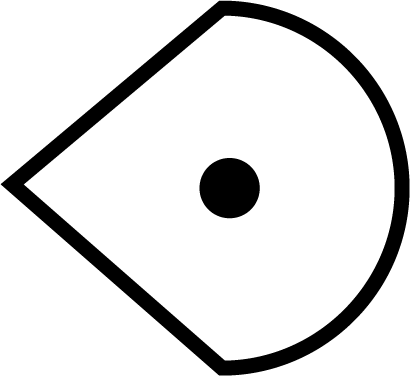
\includegraphics[width=0.8cm]{7.png}
				\end{minipage} &
				\begin{minipage}[t]{\linewidth}
					\vspace{-7pt}
					\begin{itemize}
						\item \textbf{Radar Angle Tracking}
						\begin{itemize}
							\item Jamming Target
							\item Alt. diff. ranging
						\end{itemize}
					\end{itemize}
				\end{minipage} \\
				\midrule
				\textbf{TCS-Angle Tracked Target} &
				\begin{minipage}[t]{\linewidth}
					\vspace{-7pt}
					\centering
					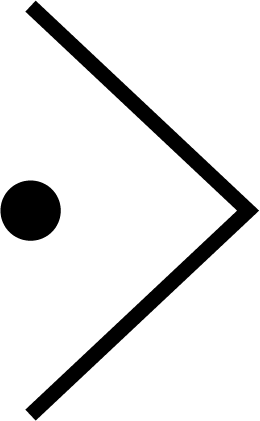
\includegraphics[width=0.55cm]{10.png}
				\end{minipage} &
				\begin{minipage}[t]{\linewidth}
					\vspace{-7pt}
					\begin{itemize}
						\item \textbf{TCS Angle Tracking}
					\end{itemize}
				\end{minipage} \\
				\midrule
				\textbf{TCS-Angle Tracked Target with Altitude Difference Ranging} &
				\begin{minipage}[t]{\linewidth}
					\vspace{-7pt}
					\centering
					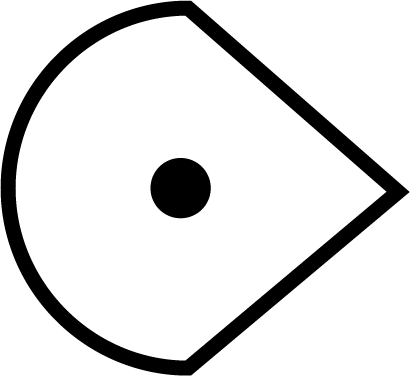
\includegraphics[width=0.8cm]{11.png}
				\end{minipage} &
				\begin{minipage}[t]{\linewidth}
					\vspace{-7pt}
					\begin{itemize}
						\item \textbf{TCS Angle Tracking}
						\begin{itemize}
							\item Alt. diff. ranging
						\end{itemize}
					\end{itemize}
				\end{minipage} \\
				\midrule
				\multicolumn{2}{c|}{\blue{D/L TARGETS}} & \textbf{Symbol Below Dot} \\
				\midrule
				\textbf{Unknown} &
				\begin{minipage}[t]{\linewidth}
					\vspace{-7pt}
					\centering
					
\includegraphics[width=0.8cm]{12.png}
				\end{minipage} &
				\begin{minipage}[t]{\linewidth}
					\vspace{-7pt}
					\begin{itemize}
						\item \textbf{D/L Track designated Unknown by Source}
					\end{itemize}
				\end{minipage} \\
				\midrule
				\textbf{Hostile} &
				\begin{minipage}[t]{\linewidth}
					\vspace{-7pt}
					\centering
					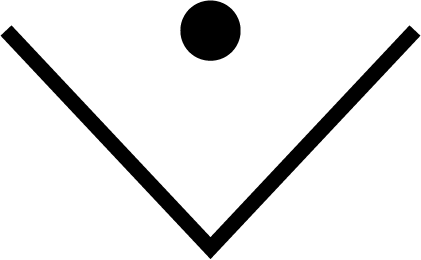
\includegraphics[width=0.8cm]{13.png}
				\end{minipage} &
				\begin{minipage}[t]{\linewidth}
					\vspace{-7pt}
					\begin{itemize}
						\item \textbf{D/L Track designated Hostile by Source}
					\end{itemize}
				\end{minipage} \\
				\midrule
				\textbf{Friendly} &
				\begin{minipage}[t]{\linewidth}
					\vspace{-7pt}
					\centering
					
\includegraphics[width=0.8cm]{14.png}
				\end{minipage} &
				\begin{minipage}[t]{\linewidth}
					\vspace{-7pt}
					\begin{itemize}
						\item \textbf{D/L Track designated Friendly by Source}
					\end{itemize}
				\end{minipage} \\
				\midrule
				\multicolumn{2}{c}{\blue{MANUAL REF POINTS}} & \\
				\midrule
				\textbf{Home base} &
				\begin{minipage}[t]{\linewidth}
					\vspace{-7pt}
					\centering
					
\includegraphics[width=0.8cm]{15.png}
				\end{minipage} &
				\begin{minipage}[t]{\linewidth}
					\vspace{-7pt}
					\begin{itemize}
						\item \textbf{Waypoint Representing}
						\begin{itemize}
							\item Home Base
							\item Carrier
							\item Airfield
						\end{itemize}
					\end{itemize}
				\end{minipage} \\
				\midrule
				\textbf{Waypoint} &
				\begin{minipage}[t]{\linewidth}
					\vspace{-7pt}
					\centering
					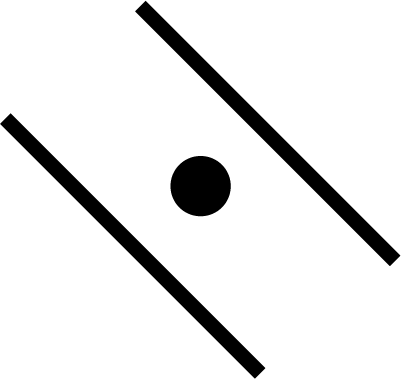
\includegraphics[width=0.8cm]{16.png}
				\end{minipage} &
				\begin{minipage}[t]{\linewidth}
					\vspace{-7pt}
					\begin{itemize}
						\item \textbf{Nav Waypoint}
						\item \textbf{Supplanted by Number}
						\begin{itemize}
							\item 1, 2, or 3
						\end{itemize}
					\end{itemize}
				\end{minipage} \\
				\midrule
				\textbf{Defended Point} &
				\begin{minipage}[t]{\linewidth}
					\vspace{-7pt}
					\centering
					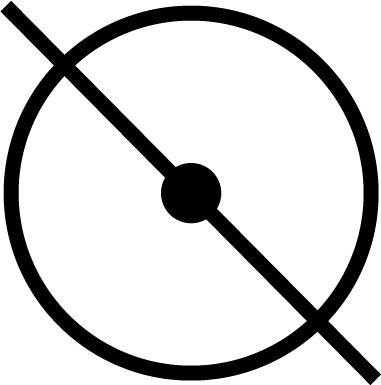
\includegraphics[width=0.8cm]{17.png}
				\end{minipage} &
				\begin{minipage}[t]{\linewidth}
					\vspace{-7pt}
					\begin{itemize}
						\item \textbf{Waypoint to Defend}
					\end{itemize}
				\end{minipage} \\
				\midrule
				\textbf{Fixed Point} &
				\begin{minipage}[t]{\linewidth}
					\vspace{-7pt}
					\centering
					
\includegraphics[width=0.8cm]{18.png}
				\end{minipage} &
				\begin{minipage}[t]{\linewidth}
					\vspace{-7pt}
					\begin{itemize}
						\item \textbf{Generic Waypoint}
					\end{itemize}
				\end{minipage} \\
				\midrule
				\textbf{Hostile Area} &
				\begin{minipage}[t]{\linewidth}
					\vspace{-7pt}
					\centering
					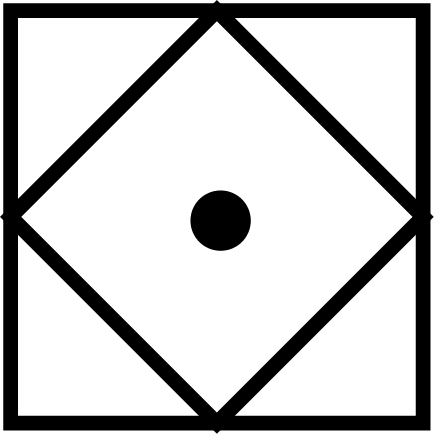
\includegraphics[width=0.8cm]{19.png}
				\end{minipage} &
				\begin{minipage}[t]{\linewidth}
					\vspace{-7pt}
					\begin{itemize}
						\item \textbf{Waypoint Indicating Hostile Area}
					\end{itemize}
				\end{minipage} \\
				\midrule
				\textbf{Surface Target} &
				\begin{minipage}[t]{\linewidth}
					\vspace{-7pt}
					\centering
					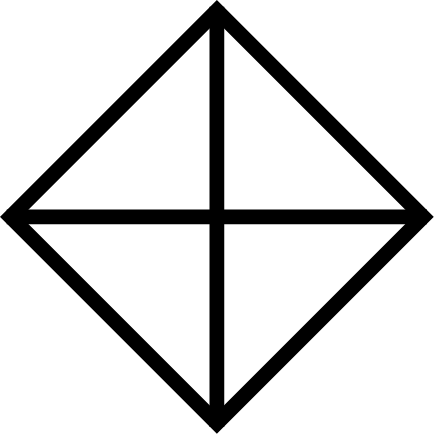
\includegraphics[width=0.8cm]{20.png}
				\end{minipage} &
				\begin{minipage}[t]{\linewidth}
					\vspace{-7pt}
					\begin{itemize}
						\item \textbf{Waypoint Indicating Surface Target}
					\end{itemize}
				\end{minipage} \\
				\midrule
				\textbf{IP} &
				\begin{minipage}[t]{\linewidth}
					\vspace{-7pt}
					\centering
					
\includegraphics[width=0.8cm]{21.png}
				\end{minipage} &
				\begin{minipage}[t]{\linewidth}
					\vspace{-7pt}
					\begin{itemize}
						\item \textbf{Initial Point}
						\begin{itemize}
							\item Waypoint for A/G engagement
						\end{itemize}
					\end{itemize}
				\end{minipage} \\
				\midrule
				\multicolumn{2}{c}{\blue{D/L REF POINTS}} & \\
				\midrule
				\textbf{Home Base} &
				\begin{minipage}[t]{\linewidth}
					\vspace{-7pt}
					\centering
					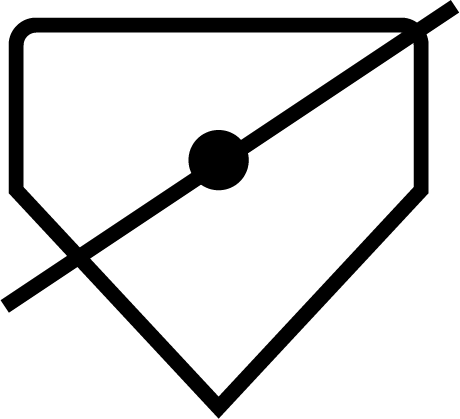
\includegraphics[width=0.8cm]{22.png}
				\end{minipage} &
				\begin{minipage}[t]{\linewidth}
					\vspace{-7pt}
					\begin{itemize}
						\item \textbf{D/L Waypoint Representing Home Base}
					\end{itemize}
				\end{minipage} \\
				\midrule
				\textbf{Waypoint} &
				\begin{minipage}[t]{\linewidth}
					\vspace{-7pt}
					\centering
					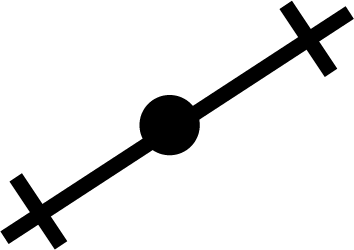
\includegraphics[width=0.8cm]{23.png}
				\end{minipage} &
				\begin{minipage}[t]{\linewidth}
					\vspace{-7pt}
					\begin{itemize}
						\item \textbf{D/L Generic Waypoint}
					\end{itemize}
				\end{minipage} \\
				\midrule
				\textbf{Data Link Fixed Point} &
				\begin{minipage}[t]{\linewidth}
					\vspace{-7pt}
					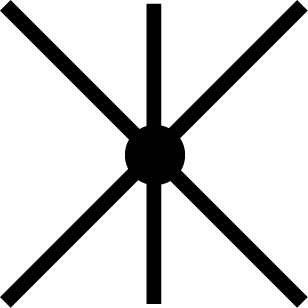
\includegraphics[width=0.8cm]{24.png}
				\end{minipage} &
				\begin{minipage}[t]{\linewidth}
					\vspace{-7pt}
					\begin{itemize}
						\item \textbf{D/L Waypoint Representing Fixed Point}
					\end{itemize}
				\end{minipage} \\
				\midrule
				\textbf{Surface Target} &
				\begin{minipage}[t]{\linewidth}
					\vspace{-7pt}
					\centering
					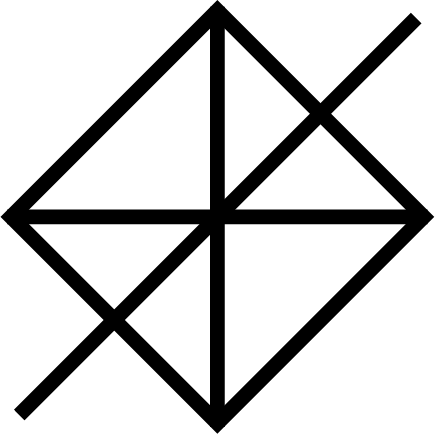
\includegraphics[width=0.8cm]{25.png}
				\end{minipage} &
				\begin{minipage}[t]{\linewidth}
					\vspace{-7pt}
					\begin{itemize}
						\item \textbf{D/L Waypoint Representing a Surface Target}
					\end{itemize}
				\end{minipage} \\
				\midrule
				\multicolumn{2}{c}{\blue{POS SYMB MODIFIERS}} & \thumbnar \\
				\midrule
				\textbf{Mandatory Attack} &
				\begin{minipage}[t]{\linewidth}
					\vspace{-7pt}
					\centering
					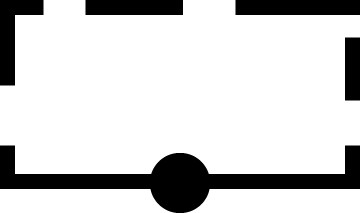
\includegraphics[width=0.8cm]{28.png}
				\end{minipage} &
				\begin{minipage}[t]{\linewidth}
					\vspace{-7pt}
					\begin{itemize}
						\item \textbf{Additional Symbology on TWS Track}
						\begin{itemize}
							\item Horizontal bar through center dot
						\end{itemize}
						\item \textbf{Selected by RIO}
						\begin{itemize}
							\item Only 1 target can be designated
							\item Guaranteed WCS priority number
						\end{itemize}
					\end{itemize}
				\end{minipage} \\
				\midrule
				\textbf{Data Link Destroy }&
				\begin{minipage}[t]{\linewidth}
					\vspace{-7pt}
					\centering
					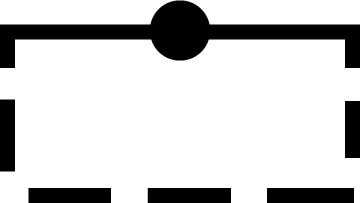
\includegraphics[width=0.8cm]{29.png}
				\end{minipage} &
				\begin{minipage}[t]{\linewidth}
					\vspace{-7pt}
					\begin{itemize}
						\item \textbf{Additional Symbology on D/L Track}
						\begin{itemize}
							\item Horizontal bar through center dot
						\end{itemize}
						\item \textbf{Selected by Source}
						\begin{itemize}
							\item No effect on WCS prioritization
						\end{itemize}
					\end{itemize}
				\end{minipage} \\
				\midrule
				\textbf{Do Not Attack} &
				\begin{minipage}[t]{\linewidth}
					\vspace{-7pt}
					\centering
					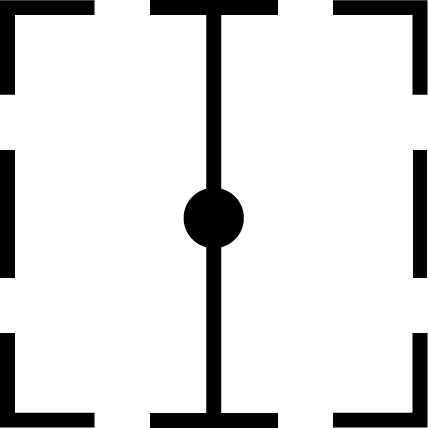
\includegraphics[width=0.8cm]{30.png}
				\end{minipage} &
				\begin{minipage}[t]{\linewidth}
					\vspace{-7pt}
					\begin{itemize}
						\item \textbf{Additional Symbology on TWS or D/L Track}
						\begin{itemize}
							\item Vertical bar through center dot
						\end{itemize}
						\item \textbf{If Set by RIO}
						\begin{itemize}
							\item Removes WCS prioritization
						\end{itemize}
					\end{itemize}
				\end{minipage} \\
				\midrule
				\textbf{Multiple Targets} &
				\begin{minipage}[t]{\linewidth}
					\vspace{-7pt}
					\centering
					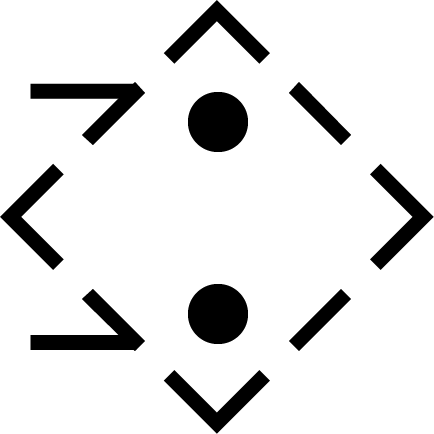
\includegraphics[width=0.8cm]{31.png}
				\end{minipage} &
				\begin{minipage}[t]{\linewidth}
					\vspace{-7pt}
					\begin{itemize}
						\item \textbf{Additional Symbology on TWS or D/L Track}
						\begin{itemize}
							\item Horizontal bar on left side of symbol
						\end{itemize}
						\item \textbf{Indicates Multiple Targets}
					\end{itemize}
				\end{minipage} \\
				\midrule
				\textbf{Data Link Challenge} &
				\begin{minipage}[t]{\linewidth}
					\vspace{-7pt}
					\centering
					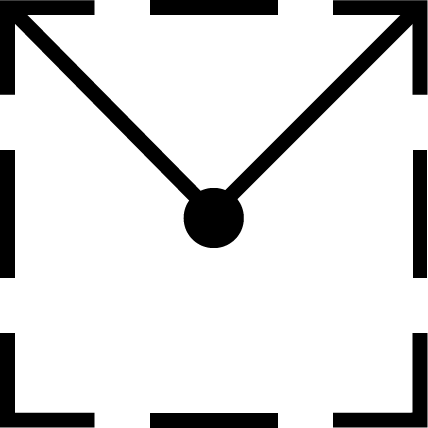
\includegraphics[width=0.8cm]{32.png}
				\end{minipage} &
				\begin{minipage}[t]{\linewidth}
					\vspace{-7pt}
					\begin{itemize}
						\item \textbf{Additional Symbology on D/L Track}
						\begin{itemize}
							\item Small \textbf{V} with center at center dot
						\end{itemize}
						\item \textbf{Command to Visually Identify}
					\end{itemize}
				\end{minipage} \\
				\midrule
				\textbf{Track Extrapolated} &
				\begin{minipage}[t]{\linewidth}
					\vspace{-7pt}
					\centering
					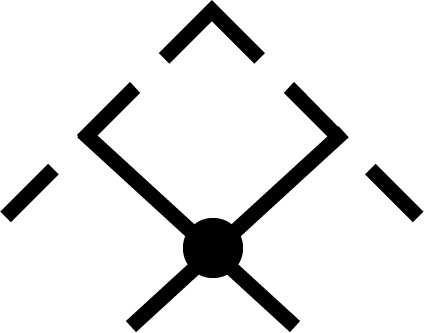
\includegraphics[width=0.8cm]{33.png}
				\end{minipage} &
				\begin{minipage}[t]{\linewidth}
					\vspace{-7pt}
					\begin{itemize}
						\item \textbf{Additional Symbology on TWS or D/L Track}
						\begin{itemize}
							\item Small \textbf{X} with center at center dot
						\end{itemize}
						\item \textbf{No Update within 8 seconds}
						\begin{itemize}
							\item Track deleted after 14 seconds
							\item Or after 2 min if track hold
						\end{itemize}
					\end{itemize}
				\end{minipage} \\
				\midrule
				\textbf{Altitude Numerics} &
				\begin{minipage}[t]{\linewidth}
					\vspace{-7pt}
					\centering
					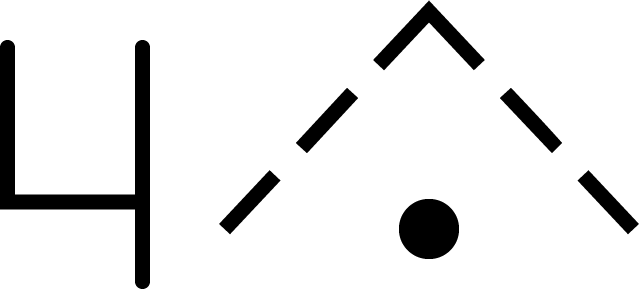
\includegraphics[width=1cm]{34.png}
				\end{minipage} &
				\begin{minipage}[t]{\linewidth}
					\vspace{-7pt}
					\begin{itemize}
						\item \textbf{Altitude to Nearest Ten Thousand}
						\begin{itemize}
							\item example: 35000-45000
						\end{itemize}
					\end{itemize}
				\end{minipage} \\
				\midrule
				\textbf{Firing Order Numerics} &
				\begin{minipage}[t]{\linewidth}
					\vspace{-7pt}
					\centering
					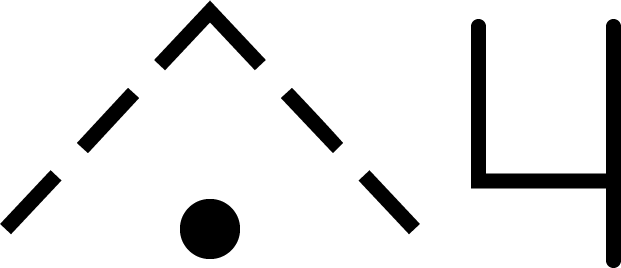
\includegraphics[width=1cm]{35.png}
				\end{minipage} &
				\begin{minipage}[t]{\linewidth}
					\vspace{-7pt}
					\begin{itemize}
						\item \textbf{Indicates AIM-54 Prioritization}
						\begin{itemize}
							\item Numbers 1-6
							\item Only in TWS
						\end{itemize}
					\end{itemize}
				\end{minipage} \\
				\midrule
				\textbf{Time-to-Impact (TTI)} &
				\begin{minipage}[t]{\linewidth}
					\vspace{-7pt}
					\centering
					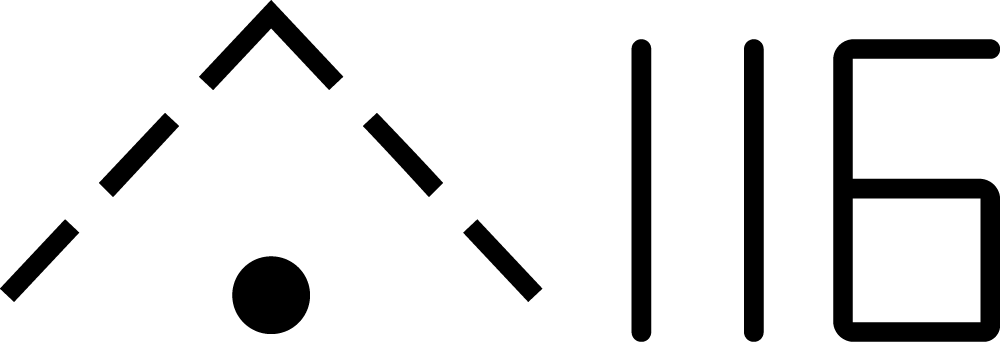
\includegraphics[width=1cm]{47.png}
				\end{minipage} &
				\begin{minipage}[t]{\linewidth}
					\vspace{-7pt}
					\begin{itemize}
						\item \textbf{After AIM-54 Launch}
						\begin{itemize}
							\item Prioritization replaced with estimated TTI
						\end{itemize}
						\item \textbf{Flashes after Pitbull}
					\end{itemize}
				\end{minipage} \\
				\midrule
				\textbf{Velocity Vector} &
				\begin{minipage}[t]{\linewidth}
					\vspace{-7pt}
					\centering
					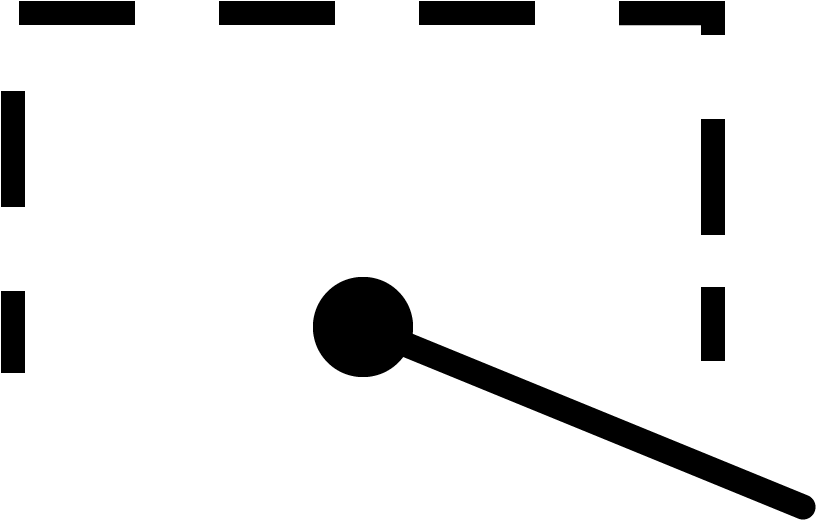
\includegraphics[width=0.8cm]{36.png}
				\end{minipage} &
				\begin{minipage}[t]{\linewidth}
					\vspace{-7pt}
					\begin{itemize}
						\item \textbf{Additional Symbology from center Dot}
						\begin{itemize}
							\item Direction represents track heading
							\item Length represents speed
						\end{itemize}
						\item \textbf{Varies with Mode}
						\begin{itemize}
							\item Ground Stabilized: true heading and ground speed
							\item Aircraft Stabilized: relative heading and velocity
						\end{itemize}
					\end{itemize}
				\end{minipage} \\
				\midrule
				\textbf{Launch Zone Vectors} &
				\begin{minipage}[t]{\linewidth}
					\vspace{-7pt}
					\centering
					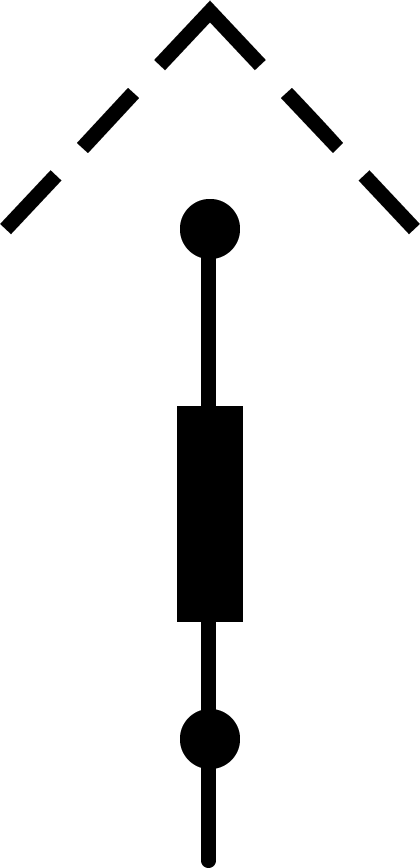
\includegraphics[width=0.8cm]{37.png}
				\end{minipage} &
				\begin{minipage}[t]{\linewidth}
					\vspace{-7pt}
					\centering
					
\includegraphics[width=5cm]{lzv.png}
				\end{minipage}
				\begin{minipage}[t]{\linewidth}
					\begin{itemize}
						\item \textbf{Additional Symbology for AIM-54}
						\begin{itemize}
							\item Selected manually by RIO
							\item Or 60 seconds from max launch
						\end{itemize}
						\item \textbf{TUMR}
						\begin{itemize}
							\item Time-Until-Minimum-Range
							\item Max: 180 seconds, 1.5 inches
						\end{itemize}
						\item \textbf{TUOR}
						\begin{itemize}
							\item Time-Until-Optimal-Range
							\item Start of bar is 8 seconds from optimum
						\end{itemize}
						\item \textbf{TUIR}
						\begin{itemize}
							\item Time-Until-In-Range
						\end{itemize}
					\end{itemize}
				\end{minipage} \\
				\midrule
				\textbf{Jamming Strobe} &
				\begin{minipage}[t]{\linewidth}
					\vspace{-7pt}
					\centering
					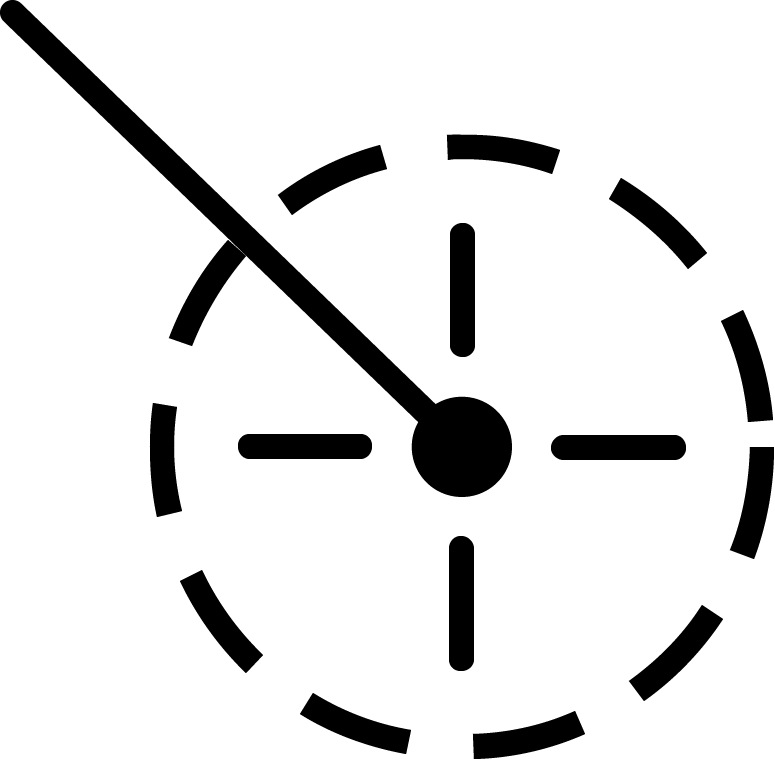
\includegraphics[width=0.8cm]{38.png}
				\end{minipage} &
				\begin{minipage}[t]{\linewidth}
					\vspace{-7pt}
					\begin{itemize}
						\item \textbf{Line from own AC towards Jammer}
					\end{itemize}
				\end{minipage} \\
				\midrule
				\textbf{Radar Antenna Scan Pattern Azimuth Limit}s &
				\begin{minipage}[t]{\linewidth}
					\vspace{-7pt}
					\centering
					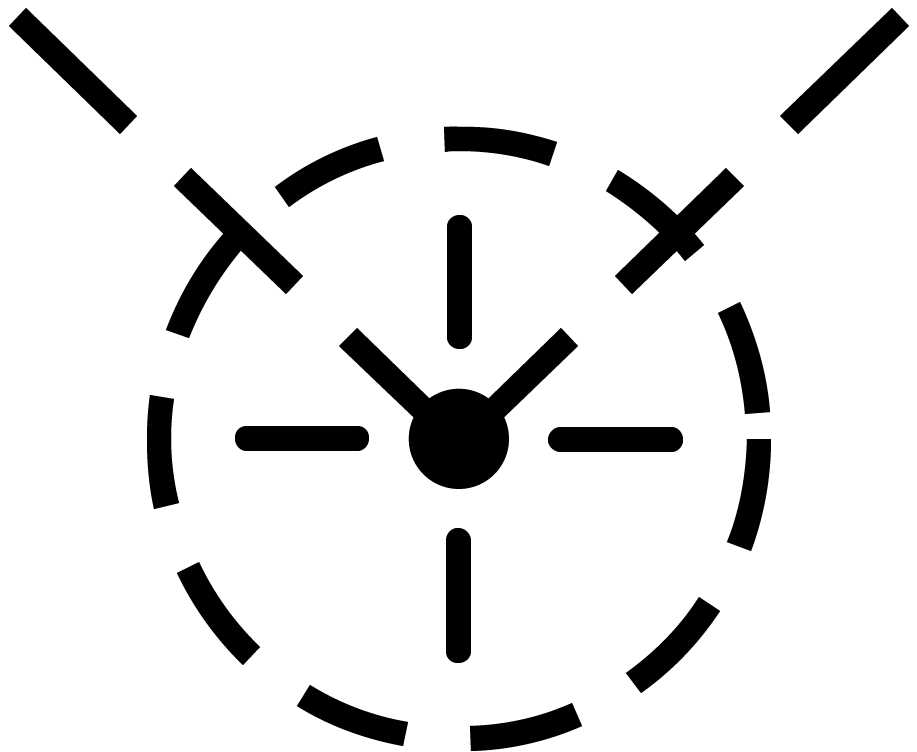
\includegraphics[width=0.8cm]{39.png}
				\end{minipage} &
				\begin{minipage}[t]{\linewidth}
					\vspace{-7pt}
					\begin{itemize}
						\item \textbf{Limits of Current Scan Azimuth}
						\item \textbf{Single Line in STT}
					\end{itemize}
				\end{minipage} \\
				\midrule
				\textbf{Data Link Jamming Strobe} &
				\begin{minipage}[t]{\linewidth}
					\vspace{-7pt}
					\centering
					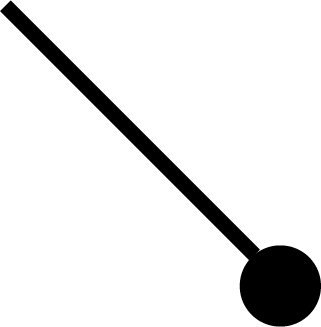
\includegraphics[width=0.8cm]{40.png}
				\end{minipage} &
				\begin{minipage}[t]{\linewidth}
					\vspace{-7pt}
					\begin{itemize}
						\item \textbf{Line from D/L point towards Jammer}
					\end{itemize}
				\end{minipage} \\
				\midrule
				\textbf{Data Link Pointer} &
				\begin{minipage}[t]{\linewidth}
					\vspace{-7pt}
					\centering
					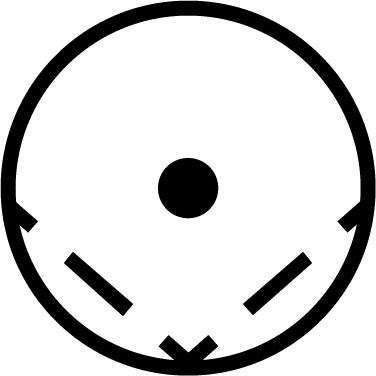
\includegraphics[width=0.8cm]{41.png}
				\end{minipage} &
				\begin{minipage}[t]{\linewidth}
					\vspace{-7pt}
					\begin{itemize}
						\item \textbf{Additional Symbology on D/L Track}
						\begin{itemize}
							\item Circle
							\item Indicates operator concern
						\end{itemize}
					\end{itemize}
				\end{minipage} \\
				\midrule
				\textbf{Data Link Priority Kill} &
				\begin{minipage}[t]{\linewidth}
					\vspace{-7pt}
					\centering
					
\includegraphics[width=0.8cm]{42.png}
				\end{minipage} &
				\begin{minipage}[t]{\linewidth}
					\vspace{-7pt}
					\begin{itemize}
						\item \textbf{Additional Symbology on D/L Track}
						\begin{itemize}
							\item Square
							\item Indicates target must be destroyed
							\item No effect on WCS prioritization
						\end{itemize}
					\end{itemize}
				\end{minipage} \\
				\midrule
				\multicolumn{2}{c}{\blue{ATTACK DISPLAY SYMBOLOGY}} & \thumbnar \\
				\midrule
				\textbf{Artificial Horizon} &
				\begin{minipage}[t]{\linewidth}
					\vspace{-7pt}
					\centering
					\includegraphics[width=0.8cm]{43.png}
				\end{minipage} &
				\begin{minipage}[t]{\linewidth}
					\vspace{-7pt}
					\begin{itemize}
						\item \textbf{Represents Pitch and Roll}
					\end{itemize}
				\end{minipage} \\
				\midrule
				\textbf{Steering Guidance Symbol} &
				\begin{minipage}[t]{\linewidth}
					\vspace{-7pt}
					\centering
					\includegraphics[width=0.8cm]{44.png}
				\end{minipage} &
				\begin{minipage}[t]{\linewidth}
					\vspace{-7pt}
					\begin{itemize}
						\item \textbf{Represents Steering Error}
						\begin{itemize}
							\item Should be placed as near as possible to center of ASE circle
						\end{itemize}
					\end{itemize}
				\end{minipage} \\
				\midrule
				\textbf{Allowable Steering Error Circle} &
				\begin{minipage}[t]{\linewidth}
					\vspace{-7pt}
					\centering
					\includegraphics[width=0.8cm]{45.png}
				\end{minipage} &
				\begin{minipage}[t]{\linewidth}
					\vspace{-7pt}
					\begin{itemize}
						\item \textbf{Indicates Allowable Steering Error for Missile Launch}
						\item \textbf{Size Varies with Geometry, Mode, Missile}
					\end{itemize}
				\end{minipage} \\
				\midrule
				\textbf{Breakaway Indication} &
				\begin{minipage}[t]{\linewidth}
					\vspace{-7pt}
					\centering
					\includegraphics[width=0.8cm]{27.png}
				\end{minipage} &
				\begin{minipage}[t]{\linewidth}
					\vspace{-7pt}
					\begin{itemize}
						\item \textbf{Appears when Target Range Less than Minimum for Selected Weapon}
					\end{itemize}
				\end{minipage} \\
				\bottomrule
			\end{longtable}
		\end{center}

		\cleardoublepage

		\section{TCS}
		\thumbtab{TCS - LANTIRN}{3}

		\subsection{OVERVIEW}

		\cleardoublepage

		\section{LANTIRN}

		\subsection{OVERVIEW}
		\begin{center}
			\begin{longtable}{l p{3cm} | p{8cm}}
				\toprule
				\textbullet & \blue{LANTIRN} \thumbnar & \textbf{L}ow \textbf{A}ltitude \textbf{N}avigation and \textbf{T}argeting \textbf{I}nfra-\textbf{R}ed for \textbf{N}ight

				\begin{minipage}[t]{\linewidth}
					\vspace{-7pt}
					\begin{itemize}
						\item \textbf{Only Targeting Pod} -- Nav pod was deleted
						\item \textbf{Incomplete Integration} -- Own control panel, supplants TCS feed
					\end{itemize}
				\end{minipage} \\
				\midrule
				\textbullet & \blue{Master Modes} \thumbnar &
				\begin{minipage}[t]{\linewidth}
					\vspace{-7pt}
					\begin{itemize}
						\item \textbf{A/G} -- Allows bomb release guidance
						\item \textbf{A/A} -- Optimized for air targets
					\end{itemize}
				\end{minipage} \\
				\midrule
				\textbullet & \blue{FOV Levels} \blue{Overview} &
				\begin{minipage}[t]{\linewidth}
					\vspace{-7pt}
					\begin{itemize}
						\item \textbf{Wide}
						\begin{itemize}
							\item \textbf{FOV} -- 5.9 deg
							\item \textbf{Slew} -- 8.5 deg/s
						\end{itemize}
						\item \textbf{Narrow}
						\begin{itemize}
							\item \textbf{FOV} -- 1.7 deg
							\item \textbf{Slew} -- 1.8 deg/s
						\end{itemize}
						\item \textbf{Expanded}
						\begin{itemize}
							\item \textbf{FOV} -- 0.8 deg
							\item \textbf{Slew} -- 0.7 deg/s
							\item \textbf{Digital Zoom} -- Degraded quality
						\end{itemize}
					\end{itemize}
				\end{minipage} \\
				\bottomrule
			\end{longtable}
		\end{center}

		\subsection{OVERVIEW - STARTUP}
		\begin{center}
			\begin{tabular}{l p{3cm} | p{8cm}}
				\toprule
				1. & \dblue{Power Switch} & \textbf{POD} \\
				\midrule
				2. & \blue{Pod Startup} \hfill\null \blue{Sequence} &
				\begin{minipage}[t]{\linewidth}
					\vspace{-7pt}
					\begin{itemize}
						\item 8 min startup sequence
						\item \textbf{MODE Switch} shows \textbf{STBY} when complete
					\end{itemize}
				\end{minipage} \\
				\midrule
				3. & \dblue{MODE Switch} & \textbf{Press} \\
				\midrule
				4. & \blue{Initialization} \hfill \null \blue{Sequence} &
				\begin{minipage}[t]{\linewidth}
					\vspace{-7pt}
					\begin{itemize}
						\item 30 sec initialization
						\item \textbf{MODE Switch} shows \textbf{OPER} when ready
					\end{itemize}
				\end{minipage} \\
				\midrule
				5. & \dblue{VIDEO Switch} & \textbf{FLIR} \\
				\midrule
				6. & \dblue{TID MODE} & \textbf{TV} \\
				\bottomrule
			\end{tabular}
		\end{center}

		\clearpage

		\subsection{OVERVIEW - POINTING MODES}
		\begin{center}
			\begin{longtable}{l p{3cm} | p{8cm}}
				\toprule
%				\textbullet & \blue{Master Modes} &
%				\begin{minipage}[t]{\linewidth}
%					\vspace{-7pt}
%					\begin{itemize}
%						\item \textbf{A/G}
%						\begin{itemize}
%							\item Optimized for ground targets
%							\item \textbf{Allows Bomb Release Guidance}
%						\end{itemize}
%						\item \textbf{A/A}
%						\begin{itemize}
%							\item Optimized for air targets
%						\end{itemize}
%					\end{itemize}
%				\end{minipage} \\
%				\midrule
%				\textbullet & \blue{FOV Levels} \blue{Overview} &
%				\begin{minipage}[t]{\linewidth}
%					\vspace{-7pt}
%					\begin{itemize}
%						\item \textbf{Wide}
%						\begin{itemize}
%							\item \textbf{FOV} -- 5.9 deg
%							\item \textbf{Slew} -- 8.5 deg/s
%						\end{itemize}
%						\item \textbf{Narrow}
%						\begin{itemize}
%							\item \textbf{FOV} -- 1.7 deg
%							\item \textbf{Slew} -- 1.8 deg/s
%						\end{itemize}
%						\item \textbf{Expanded}
%						\begin{itemize}
%							\item \textbf{FOV} -- 0.8 deg
%							\item \textbf{Slew} -- 0.7 deg/s
%							\item \textbf{Digital Zoom} -- Degraded quality
%						\end{itemize}
%					\end{itemize}
%				\end{minipage} \\
%				\midrule
				\textbullet & \blue{Sensor Modes} \blue{Overview} &
				\begin{minipage}[t]{\linewidth}
					\vspace{-7pt}
					\begin{itemize}
						\item \textbf{Contrast Lock}
						\begin{itemize}
							\item \textbf{Area Track}
							\item \textbf{Point Track}
						\end{itemize}
						\item \textbf{Q Designation}
						\begin{itemize}
							\item \textbf{Directional Q} -- QSNO / QADL / QHUD
							\item \textbf{Location Q} -- QWp / QDES
						\end{itemize}
					\end{itemize}
				\end{minipage} \\
				\midrule
				\textbullet & \blue{Directional Q} &
				\begin{minipage}[t]{\linewidth}
					\vspace{-7pt}
					\begin{itemize}
						\item \textbf{Do Not Allow Weapon Guidance}
						\item \textbf{QSNO}
						\begin{itemize}
							\item Pod slaved to \textbf{ground 15 nm in front} along own aircraft heading
						\end{itemize}
						\item \textbf{QADL}
						\begin{itemize}
							\item \textbf{Pod slaved to ADL}
							\item In A/A mode
						\end{itemize}
						\item \textbf{QHUD}
						\begin{itemize}
							\item \textbf{Pod slaved to HUD}
							\item In A/G mode
						\end{itemize}
					\end{itemize}
				\end{minipage} \\
				\midrule
				\textbullet & \blue{Location Q} &
				\begin{minipage}[t]{\linewidth}
					\vspace{-7pt}
					\begin{itemize}
						\item \textbf{Allow Weapon Guidance}
						\item \textbf{QWp}
						\begin{itemize}
							\item Pod slaved to WCS waypoint
							\item Cycled with \textbf{QWp+} / \textbf{QWp-}
						\end{itemize}
						\item \textbf{QDES}
						\begin{itemize}
							\item \textbf{Designate targets for engagement}
							\item \textbf{LANTIRN Trigger Second Detent} to designate
							\item Coordinates can be manually added to WCS for navigation
						\end{itemize}
					\end{itemize}
				\end{minipage} \\
				\bottomrule
			\end{longtable}
		\end{center}

		\clearpage

		\hypertarget{subsec:lantirnlasingdesignation}{}
		\subsection{OVERVIEW - LASING/DESIGNATION}
		\begin{center}
			\begin{longtable}{l p{3cm} | p{8cm}}
				\toprule
				\textbullet & \blue{A/G Designation} \thumbnar &
				\begin{minipage}[t]{\linewidth}
					\vspace{-7pt}
					\begin{enumerate}[label=(\alph*)]
						\item \textbf{Designate} \dotfill \textbf{Trigger Full-Action}
						\begin{itemize}
							\item Laser Fires
							\item Slant Range calculated
							\item Time-to-Go calculated
						\end{itemize}
					\end{enumerate}
				\end{minipage} \\
				\midrule
				\textbullet & \blue{Steering Cues} &
				\begin{minipage}[t]{\linewidth}
					\vspace{-7pt}
					\begin{itemize}
						\item \textbf{Automatically activated when QDES selected/designated}
						\item QDES remains even if new Q selected
						\item Cues still point towards QDES even if pod at another point
					\end{itemize}
				\end{minipage} \\
				\midrule
				\textbullet & \blue{Manual Lase} &
				\begin{minipage}[t]{\linewidth}
					\vspace{-7pt}
					\begin{enumerate}[label=(\alph*)]
						\item \textbf{Lase} \dotfill \textbf{Trigger Half-Action Hold}
					\end{enumerate}
				\end{minipage} \\
				\midrule
				\textbullet & \blue{Latched Lase} &
				\begin{minipage}[t]{\linewidth}
					\vspace{-7pt}
					\begin{itemize}
						\item \textbf{Effect} -- Lases for 60 sec
					\end{itemize}
					\begin{enumerate}[label=(\alph*)]
						\item \textbf{Activate} \dotfill \textbf{Latch Lase Button Press}
						\item \textbf{Extend} \dotfill \textbf{Latch Lase Button Press}
						\item \textbf{Deactivate} \dotfill \textbf{Trigger Half-Action}
					\end{enumerate}
				\end{minipage} \\
				\midrule
				\textbullet & \blue{Auto Lase} &
				\begin{minipage}[t]{\linewidth}
					\vspace{-7pt}
					\begin{itemize}
						\item \textbf{Effect} -- Fires from -10 to +4 sec TIMP
					\end{itemize}
					\begin{enumerate}[label=(\alph*)]
						\item \textbf{Laser Mode} \dotfill \textbf{Slider AFT Short}
						\item \textbf{Cycle A/M} \dotfill \textbf{Right 4-Way Depress}
					\end{enumerate}
				\end{minipage} \\
				\midrule
				\textbullet & \blue{Laser Notes} &
				\begin{minipage}[t]{\linewidth}
					\vspace{-7pt}
					\begin{itemize}
						\item \textbf{Always at current Pod location}
						\item Can point to different location than QDES
					\end{itemize}
				\end{minipage} \\
				\bottomrule
			\end{longtable}
		\end{center}

		\subsection{CONTROLS - PANEL}
		\begin{center}
			\begin{longtable}{l p{3cm} | p{8cm}}
				\toprule
				\textbullet & \dblue{Power Switch} &
				\begin{minipage}[t]{\linewidth}
					\vspace{-7pt}
					\begin{itemize}
						\item \textbf{OFF} -- Disables power to system
						\item \textbf{IMU} -- Only powers LANTIRN IMU \\
						\textbf{(Not Simulated in DCS)}
						\item \textbf{POD} -- Powers whole system
					\end{itemize}
				\end{minipage} \\
				\midrule
				\textbullet & \dblue{MODE Switch} &
				\begin{minipage}[t]{\linewidth}
					\vspace{-7pt}
					\begin{itemize}
						\item \textbf{STBY} -- Standby
						\item \textbf{OPER} -- Operational
					\end{itemize}
				\end{minipage} \\
				\midrule
				\textbullet & \dblue{LASER Switch} &
				\begin{minipage}[t]{\linewidth}
					\vspace{-7pt}
					\begin{itemize}
						\item \textbf{ARM} -- Arms laser
						\item \textbf{SAFE} -- Inhibits laser use
					\end{itemize}
				\end{minipage} \\
				\midrule
				\textbullet & \dblue{VIDEO Switch} &
				\begin{minipage}[t]{\linewidth}
					\vspace{-7pt}
					\begin{itemize}
						\item \textbf{FLIR} -- Displays LANTIRN FLIR on TID
						\item \textbf{TCS} -- Displays TCS video on TID
					\end{itemize}
				\end{minipage} \\
				\midrule
				\textbullet & \dblue{Indicator Light} &
				\begin{minipage}[t]{\linewidth}
					\vspace{-7pt}
					\begin{itemize}
						\item \textbf{Indicate Error States}
					\end{itemize}
				\end{minipage} \\
				\midrule
				\textbullet & \dblue{IBIT Button} &
				\begin{minipage}[t]{\linewidth}
					\vspace{-7pt}
					\begin{itemize}
						\item \textbf{Initiates Build-In-Test}
					\end{itemize}
				\end{minipage} \\
				\bottomrule
			\end{longtable}
		\end{center}

		\hypertarget{subsec:lantirncontrolsstick}{}
		\subsection{CONTROLS - STICK}
		\begin{center}
			\begin{longtable}{l p{3cm} | p{8cm}}
				\toprule
				\textbullet & \dblue{Master Mode} &
				\begin{minipage}[t]{\linewidth}
					\vspace{-7pt}
					\begin{itemize}
						\item \textbf{A/G Mode} -- \textbf{Side 2-Way FWD}
						\item \textbf{A/A Mode} -- \textbf{Side 2-Way AFT}
					\end{itemize}
				\end{minipage} \\
				\midrule
				\textbullet & \dblue{Slew} & \textbf{Center Slew Hat} \\
				\midrule
				\textbullet & \dblue{WHOT/BHOT} & \textbf{Center Slew Hat Depress} \\
				\midrule
				\textbullet & \dblue{Contrast Track} &
				\begin{minipage}[t]{\linewidth}
					\vspace{-7pt}
					\begin{itemize}
						\item \textbf{Point Track} -- \textbf{Left 4-Way Up}
						\item \textbf{Area Track} -- \textbf{Left 4-Way Down}
					\end{itemize}
				\end{minipage} \\
				\midrule
				\textbullet & \dblue{Q Select} &
				\begin{minipage}[t]{\linewidth}
					\vspace{-7pt}
					\begin{itemize}
						\item \textbf{QADL/QHUD} -- \textbf{Right 4-Way Up}
						\item \textbf{QDES} -- \textbf{Right 4-Way Right}
						\item \textbf{QSNO} -- \textbf{Right 4-Way Down}
					\end{itemize}
				\end{minipage} \\
				\midrule
				\textbullet & \dblue{Declutter} & \textbf{Right 4-Way Depress} \\
				\midrule
				\textbullet & \dblue{Zoom Level} & \textbf{FOV Button} \\
				\midrule
				\textbullet & \dblue {Cycle Gain}\dblue{Control Mode} &  \textbf{Slider FWD short} \\
				\midrule
				\textbullet & \dblue{Manual Gain} \dblue{Control} &
				\begin{minipage}[t]{\linewidth}
					\vspace{-7pt}
					\begin{enumerate}[label=(\alph*)]
						\item \textbf{Slider} \dotfill \textbf{FWD long}
						\item \textbf{Gain} \dotfill \textbf{Right 4-Way Up/Down} \\
						\textbf{Level} \dotfill \textbf{Right 4-Way Left/Right}
					\end{enumerate}
				\end{minipage} \\
				\midrule
				\textbullet & \dblue{Laser Code} &
				\begin{minipage}[t]{\linewidth}
					\vspace{-7pt}
					\begin{enumerate}[label=(\alph*)]
						\item \textbf{Slider} \dotfill \textbf{AFT short}
						\item \textbf{Select Digit} \dotfill \textbf{Right 4-Way Left/Right}
						\item \textbf{Change Digit} \dotfill \textbf{Right 4-Way Up/Down}
					\end{enumerate}
				\end{minipage} \\
				\midrule
				\textbullet & \dblue{Focus Control} &
				\begin{minipage}[t]{\linewidth}
					\vspace{-7pt}
					\begin{enumerate}[label=(\alph*)]
						\item \textbf{Slider} \dotfill \textbf{AFT hold}
						\item \textbf{Right 4-Way} \dotfill \textbf{Up/Down}
					\end{enumerate}
				\end{minipage} \\
				\midrule
				\textbullet & \dblue{Manual Lase} & \textbf{Trigger Half-Action} \\
				\midrule
				\textbullet & \dblue{Latched Laser} & \textbf{Latched Laser Fire Button} \\
				\midrule
				\textbullet & \dblue{Designate} \dblue{QDES} & \textbf{Trigger Full-Action} \\
				\bottomrule
			\end{longtable}
		\end{center}

		\clearpage

		\subsection{DISPLAY}
		\begin{center}
			\begin{longtable}{l p{3cm} | p{8cm}}
				\toprule
				\textbullet & \blue{Top Left} \thumbnar &
				\begin{minipage}[t]{\linewidth}
					\vspace{-7pt}
					\begin{itemize}
						\item \textbf{Own Aircraft Datablock}
						\begin{itemize}
							\item \textbf{Lat} -- deg:min.dec
							\item \textbf{Long} -- deg:min.dec
							\item \textbf{ALT} -- Altitude (ft)
							\item \textbf{KGS} -- Knots Ground Speed
							\item \textbf{DIVE} -- Dive Angle (deg)
						\end{itemize}
					\end{itemize}
				\end{minipage} \\
				\midrule
				\textbullet & \blue{Mid Left} &
				\begin{minipage}[t]{\linewidth}
					\vspace{-7pt}
					\begin{itemize}
						\item \textbf{Sensor Mode} -- \textbf{WHOT} / \textbf{BHOT}
						\item \textbf{Gain Control} -- \textbf{Auto} / \textbf{Manual}
					\end{itemize}
				\end{minipage} \\
				\midrule
				\textbullet & \blue{Bottom Left} &
				\begin{minipage}[t]{\linewidth}
					\vspace{-7pt}
					\begin{itemize}
						\item \textbf{Pod Info Datablock}
						\begin{itemize}
							\item \textbf{SRA} -- Slant Range
							\item \textbf{AZ} -- Pod LoS Azimuth L/R
							\item \textbf{EL} -- Pod LoS Elevation
							\item \textbf{Time} -- UTC Time
							\item \textbf{IBIT} -- Codes
						\end{itemize}
					\end{itemize}
				\end{minipage} \\
				\midrule
				\textbullet & \blue{Bottom Center } &
				\begin{minipage}[t]{\linewidth}
					\vspace{-7pt}
					\begin{itemize}
						\item \textbf{Master Mode} -- \textbf{A/A} / \textbf{A/G}
						\item \textbf{Track Mode} -- \textbf{AREA} / \textbf{POINT} / \textbf{Q}
						\item \textbf{Current Weapon}
						\item \textbf{Laser Code}
						\item \textbf{L}
						\begin{itemize}
							\item \textbf{Steady} -- Laser Armed
							\item \textbf{Flashing} -- Laser Firing
						\end{itemize}
					\end{itemize}
				\end{minipage} \\
				\midrule
				\textbullet & \blue{Bottom Right} &
				\begin{minipage}[t]{\linewidth}
					\vspace{-7pt}
					\begin{itemize}
						\item \textbf{Q Datablock}
						\begin{itemize}
							\item \textbf{TTG} -- Time-To-Go
							\item \textbf{B/R} -- Bearing and Range
							\item \textbf{ELEV} -- Elevation (ft) of Q
							\item \textbf{Lat} -- deg:min:dec
							\item \textbf{Long} -- deg:min:dec
						\end{itemize}
					\end{itemize}
				\end{minipage} \\
				\midrule
				\textbullet & \blue{Mid Center} &
				\begin{minipage}[t]{\linewidth}
					\vspace{-7pt}
					\begin{itemize}
						\item \textbf{Crosshair}
						\begin{itemize}
							\item \textbf{Bounding Box} -- Indicates currently tracked target in point mode
							\item \textbf{Zoom Boxes} -- Indicates next zoom levels
							\item \textbf{FLIR Pointing Cue} -- Shows Pod LoS, screen center indicates straight down
						\end{itemize}
					\end{itemize}
				\end{minipage} \\
				\midrule
				\textbullet & \blue{Mid Right} &
				\begin{minipage}[t]{\linewidth}
					\vspace{-7pt}
					\begin{itemize}
						\item \textbf{Bomb Rlease Cue}
						\begin{itemize}
							\item Only shown if current Q is \textbf{QDES}, with valid weapon selected
							\item \textbf{TREL} -- Time to release
							\item \textbf{TIMP} -- Time to Impact (after release)
						\end{itemize}
					\end{itemize}
				\end{minipage} \\
				\midrule
				\textbullet & \blue{Top Center} &
				\begin{minipage}[t]{\linewidth}
					\vspace{-7pt}
					\begin{itemize}
						\item \textbf{Steering Guidance to Q}
						\begin{itemize}
							\item Relative bearing L/R to commanded heading
						\end{itemize}
					\end{itemize}
				\end{minipage} \\
				\bottomrule
			\end{longtable}
		\end{center}

		\cleardoublepage

		\section{A/G WEAPONS}
		\thumbtab{A/G}{4}

		\subsection{A/G WEAPON SETTINGS - OVERVIEW}
		\begin{center}
			\begin{longtable}{l p{3cm} | p{8cm}}
				\toprule
				\textbullet & \dblue{WPN TYPE} &
				\begin{minipage}[t]{\linewidth}
					\vspace{-7pt}
					\begin{itemize}
						\item \textbf{Selects Weapon Type}
						\begin{itemize}
							\item Configures WCS for selected weapon
							\item Refer to Kneeboard for list of mounted weapons
							\item Mk-81 / 82 / 83 have both \textbf{L} and \textbf{H} option refering to high and low drag
						\end{itemize}
					\end{itemize}
				\end{minipage} \\
				\midrule
				\textbullet & \dblue{DLVY MODE} &
				\begin{minipage}[t]{\linewidth}
					\vspace{-7pt}
					\begin{itemize}
						\item \textbf{STP-SGL} -- Single weapon per press
						\item \textbf{STP-PRS} Single pair per press
						\item \textbf{RPL-SGL} -- QTY of weapons per press
						\item \textbf{RPL-PRS} -- QTY of pairs per press
					\end{itemize}
				\end{minipage} \\
				\midrule
				\textbullet & \dblue{DLVY OPTNS} &
				\begin{minipage}[t]{\linewidth}
					\vspace{-7pt}
					\begin{itemize}
						\item \textbf{INTERVAL} -- Interval in ms
						\item \textbf{QTY} -- Number of stores to be released
					\end{itemize}
				\end{minipage} \\
				\midrule
				\textbullet & \dblue{MECH FUZE} &
				\begin{minipage}[t]{\linewidth}
					\vspace{-7pt}
					\begin{itemize}
						\item \textbf{NOSE} -- Arms nose fuze
						\item \textbf{SAFE} -- Inhibits arming of fuzes
						\item \textbf{NOSE/TAIL} -- Arms both fuzes
					\end{itemize}
				\end{minipage} \\
				\midrule
				\textbullet & \dblue{ELEC FUZE} &
				\begin{minipage}[t]{\linewidth}
					\vspace{-7pt}
					\begin{itemize}
						\item \textbf{SAFE} -- Inhibits electrical bomb fuzing
						\item \textbf{VT} -- Sets air-burst mode at preset burst height for compatible stores
						\item \textbf{INST} -- Sets instantaneous burst mode
						\item \textbf{DLY 1} -- Sets preset time delay 1
						\item \textbf{DLY 2} -- Sets preset time delay 2
					\end{itemize}
				\end{minipage} \\
				\midrule
				\textbullet & \dblue{STA SEL} &
				\begin{minipage}[t]{\linewidth}
					\vspace{-7pt}
					\begin{itemize}
						\item \textbf{Selects Stations for Employment/Jettison}
						\begin{itemize}
							\item Set to \textbf{SEL} to activate a pylon
							\item Stations 1 \& 8 should be set to \textbf{B} for selection
							\item Station 1 \& 8 \textbf{SW} was used for Sidewinder jettison, is now inoperable
						\end{itemize}
					\end{itemize}
				\end{minipage} \\
				\midrule
				\textbullet & \dblue{TANK JETT} &
				\begin{minipage}[t]{\linewidth}
					\vspace{-7pt}
					\begin{itemize}
						\item \textbf{Allows Drop Tank Jettison}
					\end{itemize}
				\end{minipage} \\
				\midrule
				\textbullet & \dblue{SEL JETT} &
				\begin{minipage}[t]{\linewidth}
					\vspace{-7pt}
					\begin{itemize}
						\item \textbf{JETT} -- Selective jettison
						\item \textbf{SAFE} -- Inhibits jettison
						\item \textbf{AUX} -- Backup mode
					\end{itemize}
				\end{minipage} \\
				\midrule
				\textbullet & \dblue{JETT OPTIONS} &
				\begin{minipage}[t]{\linewidth}
					\vspace{-7pt}
					\begin{itemize}
						\item \textbf{MER TER} -- Jettisons ejector racks
						\item \textbf{WPNS} -- Jettisons weapons only
					\end{itemize}
				\end{minipage} \\
				\midrule
				\textbullet & \dblue{ATTK MODE} &
				\begin{minipage}[t]{\linewidth}
					\vspace{-7pt}
					\begin{itemize}
						\item \textbf{CCMPTR TGT}
						\begin{itemize}
							\item \textbf{Computer Target} -- Similar to CCRP
						\end{itemize}
						\item \textbf{CMPTR IP}
						\begin{itemize}
							\item \textbf{Computer initial point}
							\item Extended \textbf{CMPTR TGT} mode using known IP
							\item For use when target hard to spot visually but close to landmark
						\end{itemize}
						\item \textbf{CMPTR PLT}
						\begin{itemize}
							\item \textbf{Computer Pilot} -- similar to CCIP
						\end{itemize}
						\item \textbf{MAN}
						\begin{itemize}
							\item \textbf{Manual} -- HUD displays pipper
							\item Backup mode
						\end{itemize}
						\item \textbf{D/L BOMB}
						\begin{itemize}
							\item \textbf{Data-Link Bomb} -- Automatic mode steered by D/L cues
							\item \textbf{Not Implemented in DCS}
						\end{itemize}
					\end{itemize}
				\end{minipage} \\
				\bottomrule
			\end{longtable}
		\end{center}


		\subsection{SELECTIVE ORNANCE JETTISON}
		\begin{center}
			\begin{tabular}{l p{3cm} | p{8cm}}
				\toprule
				1. & \blue{Pilot Conditions} &
				\begin{minipage}[t]{\linewidth}
					\vspace{-7pt}
					\begin{itemize}
						\item \textbf{MASTER ARM} \dotfill \textbf{ON}
					\end{itemize}
				\end{minipage} \\
				\midrule
				2. & \dblue{RIO Conditions} &
				\begin{minipage}[t]{\linewidth}
					\vspace{-7pt}
					\begin{itemize}
						\item \textbf{Desired Stations} \dotfill \textbf{Selected}
						\item \textbf{JETT OPTIONS} \dotfill \textbf{As Desired}
					\end{itemize}
				\end{minipage} \\
				\midrule
				3. & \dblue{Jettison} &
				\begin{minipage}[t]{\linewidth}
					\vspace{-7pt}
					\begin{enumerate}[label=(\alph*)]
						\item \textbf{SEL JETT Guard} \dotfill \textbf{Flipped}
						\item \textbf{SEL JETT Switch} \dotfill \textbf{JETT}
					\end{enumerate}
				\end{minipage} \\
				\bottomrule
			\end{tabular}
		\end{center}

		\subsection{M61 GUN}
		\begin{center}
			\begin{tabular}{l p{3cm} | p{8cm}}
				\toprule
				1. & \blue{Pilot Conditions} &
				\begin{minipage}[t]{\linewidth}
					\vspace{-7pt}
					\begin{itemize}
						\item \textbf{MASTER ARM} \dotfill \textbf{ON}
						\item \textbf{HUD} \dotfill \textbf{A/G}
						\item \textbf{WEAPON SELECTOR} \dotfill \textbf{GUNS}
						\item \textbf{Wing Sweep} \dotfill \textbf{BOMB}
					\end{itemize}
				\end{minipage} \\
				\midrule
				2. & \blue{Employment} &
				\begin{minipage}[t]{\linewidth}
					\vspace{-7pt}
					\begin{enumerate}[label=(\alph*)]
						\item \textbf{Dive} \dotfill 20-30 deg
						\item \textbf{Pipper} \dotfill on target
						\item \textbf{TRIGGER} \dotfill \textbf{FIRE}
					\end{enumerate}
				\end{minipage} \\
				\midrule
				\textbullet & \blue{Note: TCS} &
				\begin{minipage}[t]{\linewidth}
					\vspace{-7pt}
					\begin{itemize}
						\item TCS slaved to radar impact point
						\item Rio can select \textbf{NAR} or \textbf{WIDE}
					\end{itemize}
				\end{minipage} \\
				\bottomrule
			\end{tabular}
		\end{center}

		\subsection{FFAR / ZUNI ROCKETS}
		\begin{center}
			\begin{tabular}{l p{3cm} | p{8cm}}
				\toprule
				1. & \dblue{RIO Conditions} &
				\begin{minipage}[t]{\linewidth}
					\vspace{-7pt}
					\begin{itemize}
						\item \textbf{WPN TYP} \dotfill \textbf{LAU-10}
						\item \textbf{Attack Mode} \dotfill \textbf{Pilot Attack}
						\item \textbf{Deliver Mode} \dotfill \textbf{RPL-SGL}
						\item \textbf{Mechanical Fuze} \dotfill \textbf{NOSE}
						\item \textbf{Electronic Fuze} \dotfill \textbf{INST}
						\item \textbf{Delivery Options} \dotfill \textbf{As Desired}
						\item \textbf{Stations} \dotfill \textbf{Armed}
					\end{itemize}
				\end{minipage} \\
				\midrule
				2. & \blue{Pilot Conditions} &
				\begin{minipage}[t]{\linewidth}
					\vspace{-7pt}
					\begin{itemize}
						\item \textbf{MASTER ARM} \dotfill \textbf{ON}
						\item \textbf{HUD} \dotfill \textbf{A/G}
						\item \textbf{WEAPON SELECTOR} \dotfill \textbf{OFF}
						\item \textbf{Stations} \dotfill verify selected
						\item \textbf{Wing Sweep} \dotfill \textbf{BOMB}
					\end{itemize}
				\end{minipage} \\
				\midrule
				3. & \blue{Employment} &
				\begin{minipage}[t]{\linewidth}
					\vspace{-7pt}
					\begin{enumerate}[label=(\alph*)]
						\item \textbf{Dive} \dotfill 20-30 deg
						\item \textbf{Pipper} \dotfill on target
						\item \textbf{TRIGGER} \dotfill \textbf{FIRE}
					\end{enumerate}
				\end{minipage} \\
				\bottomrule
			\end{tabular}
		\end{center}

		\subsection{UNGUIDED BOMB - CCIP}
		\begin{center}
			\begin{tabular}{l p{3cm} | p{8cm}}
				\toprule
				1. & \dblue{RIO Conditions} &
				\begin{minipage}[t]{\linewidth}
					\vspace{-7pt}
					\begin{itemize}
						\item \textbf{WPN TYP} \dotfill \textbf{MK-8X}
						\item \textbf{Attack Mode} \dotfill \textbf{Pilot Attack}
						\item \textbf{Deliver Mode} \dotfill \textbf{STP-PRS}
						\item \textbf{Mechanical Fuze} \dotfill \textbf{NOSE}
						\item \textbf{Electronic Fuze} \dotfill \textbf{INST}
						\item \textbf{Delivery Options} \dotfill \textbf{As Desired}
						\item \textbf{Stations} \dotfill \textbf{Armed}
					\end{itemize}
				\end{minipage} \\
				\midrule
				2. & \blue{Pilot Conditions} &
				\begin{minipage}[t]{\linewidth}
					\vspace{-7pt}
					\begin{itemize}
						\item \textbf{MASTER ARM} \dotfill \textbf{ON}
						\item \textbf{HUD} \dotfill \textbf{A/G}
						\item \textbf{WEAPON SELECTOR} \dotfill \textbf{OFF}
						\item \textbf{Stations} \dotfill verify selected
						\item \textbf{Wing Sweep} \dotfill \textbf{BOMB}
					\end{itemize}
				\end{minipage} \\
				\midrule
				3. & \blue{Employment} &
				\begin{minipage}[t]{\linewidth}
					\vspace{-7pt}
					\begin{enumerate}[label=(\alph*)]
						\item \textbf{Dive} \dotfill 40 deg
						\item \textbf{Pipper} \dotfill on target
						\item \textbf{STORE RELEASE} \dotfill \textbf{Press and Hold}
					\end{enumerate}
				\end{minipage} \\
				\bottomrule
			\end{tabular}
		\end{center}

		\subsection{UNGUIDED BOMB - CCRP}
		\begin{center}
			\begin{tabular}{l p{3cm} | p{8cm}}
				\toprule
				1. & \dblue{RIO Conditions} &
				\begin{minipage}[t]{\linewidth}
					\vspace{-7pt}
					\begin{itemize}
						\item \textbf{WPN TYP} \dotfill \textbf{MK-8X}
						\item \textbf{Attack Mode} \dotfill \textbf{Target Attack}
						\item \textbf{Deliver Mode} \dotfill \textbf{STP-PRS}
						\item \textbf{Mechanical Fuze} \dotfill \textbf{NOSE}
						\item \textbf{Electronic Fuze} \dotfill \textbf{INST}
						\item \textbf{Delivery Options} \dotfill \textbf{As Desired}
						\item \textbf{Stations} \dotfill \textbf{Armed}
					\end{itemize}
				\end{minipage} \\
				\midrule
				2. & \blue{Pilot Conditions} &
				\begin{minipage}[t]{\linewidth}
					\vspace{-7pt}
					\begin{itemize}
						\item \textbf{MASTER ARM} \dotfill \textbf{ON}
						\item \textbf{HUD} \dotfill \textbf{A/G}
						\item \textbf{WEAPON SELECTOR} \dotfill \textbf{OFF}
						\item \textbf{Stations} \dotfill verify selected
						\item \textbf{Wing Sweep} \dotfill \textbf{BOMB}
					\end{itemize}
				\end{minipage} \\
				\midrule
				3. & \blue{Designation} &
				\begin{minipage}[t]{\linewidth}
					\vspace{-7pt}
					\begin{enumerate}[label=(\alph*)]
						\item \textbf{Slew Diamond} \dotfill \textbf{VSL HI/LO}
						\item \textbf{Designate} \dotfill \textbf{PAL}
					\end{enumerate}
				\end{minipage} \\
				\midrule
				4. & \blue{Employment} &
				\begin{minipage}[t]{\linewidth}
					\vspace{-7pt}
					\begin{enumerate}[label=(\alph*)]
						\item \textbf{Flight Path} \dotfill Straight, Level
						\item \textbf{Vel Vector} \dotfill on Bomb Fall Line
					\end{enumerate}
					When Solution Cue meets Velocity Vector
					\begin{enumerate}[label=(\alph*), resume]
						\item \textbf{STORE RELEASE} \dotfill \textbf{Press and Hold}
					\end{enumerate}
				\end{minipage} \\
				\bottomrule
			\end{tabular}
		\end{center}

		\clearpage

		\subsection{LASER GUIDED BOMB}
		\begin{center}
			\begin{longtable}{l p{3cm} | p{8cm}}
				\toprule
				1. & \dblue{LANTIRN} \dblue{PREP} &
				\begin{minipage}[t]{\linewidth}
					\vspace{-7pt}
					\begin{enumerate}[label=(\alph*)]
						\item \textbf{Target Pod Power} \dotfill \textbf{POD}
						\begin{itemize}
							\item Warm up takes approx. 8 min
							\item Automatically switches to \textbf{STANDBY}
						\end{itemize}
						\item \textbf{Laser Code} \dotfill as desired
						\begin{itemize}
							\item \textbf{MUST BE SET ON THE GROUND}
							\item \textbf{Default:} 1688
						\end{itemize}
						\item \textbf{LANTIRN Mode} \dotfill \textbf{OPERATE}
						\begin{itemize}
							\item \textbf{STANDBY} caution will flash for 30 s
							\item Then switches to \textbf{OPER}
						\end{itemize}
						\item \textbf{VIDEO Switch} \dotfill \textbf{FLIR}
						\item \textbf{TID Mode} \dotfill \textbf{TV}
					\end{enumerate}
				\end{minipage} \\
				\midrule
				2. & \dblue{RIO Conditions} &
				\begin{minipage}[t]{\linewidth}
					\vspace{-7pt}
					\begin{itemize}
						\item \textbf{WPN TYP} \dotfill \textbf{GBU-XX}
						\item \textbf{Attack Mode} \dotfill \textbf{Manual}
						\item \textbf{Deliver Mode} \dotfill \textbf{STP-SGL}
						\item \textbf{Mechanical Fuze} \dotfill \textbf{NOSE}
						\item \textbf{Electronic Fuze} \dotfill \textbf{INST}
						\item \textbf{Delivery Options} \dotfill \textbf{As Desired}
						\item \textbf{Stations} \dotfill \textbf{Armed}
					\end{itemize}
				\end{minipage} \\
				\midrule
				3. & \blue{Pilot Conditions} &
				\begin{minipage}[t]{\linewidth}
					\vspace{-7pt}
					\begin{itemize}
						\item \textbf{MASTER ARM} \dotfill \textbf{ON}
						\item \textbf{HUD} \dotfill \textbf{A/G}
						\item \textbf{WEAPON SELECTOR} \dotfill \textbf{OFF}
						\item \textbf{VDI Mode} \dotfill \textbf{TV}
						\item \textbf{Stations} \dotfill verify selected
						\item \textbf{Wing Sweep} \dotfill \textbf{BOMB}
					\end{itemize}
				\end{minipage} \\
				\midrule
				4. & \dblue{Slew LANTIRN} &
				 \hyperlink{subsec:lantirncontrolsstick}{\textbf{Refer to LANTIRN Control Section}}

				\begin{minipage}[t]{\linewidth}
					\vspace{-7pt}
					\begin{itemize}
						\item \textbf{Slave to WYPT} \dotfill \textbf{Left-4-Way RIGHT}
						\item \textbf{QSNO (Snowplow)} \dotfill \textbf{S4 HAT Down}
						\item \textbf{Toggle FOV} \dotfill \textbf{LANTIRN Toggle FOV}
						\item \textbf{Slew} \dotfill \textbf{LANTIRN Stick}
						\item \textbf{Area Track} \dotfill \textbf{Left-4-Way UP}
						\item \textbf{Point Track} \dotfill \textbf{Left-4-Way Down}
						\item \textbf{Undesignate} \dotfill \textbf{LANTIRN Undesignate}

					\end{itemize}
				\end{minipage} \\
				\midrule
				4. & \dblue{Designate} & \hyperlink{subsec:lantirnlasingdesignation}{\textbf{Refer to LANTIRN Designation Section}}

				\begin{minipage}[t]{\linewidth}
					\vspace{-7pt}
					\begin{enumerate}[label=(\alph*)]
						\item \textbf{Designate} \dotfill \textbf{Trigger Full-Action}
						\begin{itemize}
							\item Slant Range calculated
							\item Time-to-Go calculated
						\end{itemize}
					\end{enumerate}
					\textbf{Once Time-to-Realease (TREL) is 0}
					\begin{enumerate}[label=(\alph*), resume]
						\item \textbf{Auto-Lase} \dotfill If selected: lases 10s to impact
						\item \textbf{Manual Lase} \dotfill \textbf{Trigger Full-Action}
						\item \textbf{While Lasing} \dotfill \textbf{L} blinks
					\end{enumerate}
				\end{minipage} \\
				\midrule
				5. & \blue{Employment} & \textbf{Once Time-to-Realease (TREL) is 0}
				\begin{minipage}[t]{\linewidth}
					\vspace{-7pt}
					\begin{enumerate}[label=(\alph*)]
						\item \textbf{STORE RELEASE} \dotfill \textbf{Press and Hold}
						\item \textbf{Flight Path} \dotfill Gentle right-hand turn \\
						\hfill (to prevent masking)
					\end{enumerate}
				\end{minipage} \\
				\bottomrule
			\end{longtable}
		\end{center}

		\subsection{TALD DECOYS}
		\begin{center}
			\begin{tabular}{l p{3cm} | p{8cm}}
				\toprule
				1. & \dblue{RIO Conditions} &
				\begin{minipage}[t]{\linewidth}
					\vspace{-7pt}
					\begin{itemize}
						\item \textbf{WPN TYP} \dotfill \textbf{TALD}
						\item \textbf{Deliver Mode} \dotfill \textbf{STP-SGL}
						\item \textbf{Delivery Options} \dotfill \textbf{As Desired}
						\item \textbf{Stations} \dotfill \textbf{Armed}
					\end{itemize}
				\end{minipage} \\
				\midrule
				2. & \blue{Pilot Conditions} &
				\begin{minipage}[t]{\linewidth}
					\vspace{-7pt}
					\begin{itemize}
						\item \textbf{MASTER ARM} \dotfill \textbf{ON}
						\item \textbf{HUD} \dotfill \textbf{A/G}
						\item \textbf{WEAPON SELECTOR} \dotfill \textbf{OFF}
						\item \textbf{HSD Mode} \dotfill \textbf{TID}
						\item \textbf{Stations} \dotfill verify selected
					\end{itemize}
				\end{minipage} \\
				\midrule
				3. & \blue{Employment} &
				\begin{minipage}[t]{\linewidth}
					\vspace{-7pt}
					\begin{enumerate}[label=(\alph*)]
						\item \textbf{Flight Path} \dotfill High / Fast
						\item \textbf{RWR} \dotfill Monitor to locate emitters
						\item \textbf{STORE RELEASE} \dotfill \textbf{Press and Hold}
					\end{enumerate}
				\end{minipage} \\
				\bottomrule
			\end{tabular}
		\end{center}



		\cleardoublepage

		\section{A/A WEAPONS}
		\thumbtab{A/A}{5}

		\subsection{M61 GUN - OVERVIEW}
		\begin{center}
			\begin{longtable}{l p{3cm} | p{8cm}}
				\toprule
				\textbullet & \blue{GUN RATE} \hfill\null \blue{Button} &
				\begin{minipage}[t]{\linewidth}
					\vspace{-7pt}
					\begin{itemize}
						\item \textbf{Cycles Gun Rate}
						\begin{itemize}
							\item \textbf{HIGH} -- 6000 rpm
							\item \textbf{LOW} -- 4000 rpm
						\end{itemize}
					\end{itemize}
				\end{minipage} \\
				\midrule
				\textbullet & \blue{A/A Gun Modes} &
				\begin{minipage}[t]{\linewidth}
					\vspace{-7pt}
					\begin{itemize}
						\item \textbf{RTGS}
						\begin{itemize}
							\item \textbf{Real-Time Gunsight Mode}
							\item Selected automatically with guns
							\item \textbf{If No WCS Data Available} displays bullet location at 2000 ft with diamond and 1000 ft with pipper
							\item \textbf{If WCS Data Available} pipper displays bullet location at targets current range out to 4000 ft
						\end{itemize}
						\item \textbf{MANUAL}
						\begin{itemize}
							\item Fixed manual pipper
							\item Adjust with \textbf{GUN ELEV} knob
							\item Press \textbf{CAGE/SEAM} to select
						\end{itemize}
					\end{itemize}
				\end{minipage} \\
				\midrule
				\textbullet & \blue{CAGE/SEAM}  \hfill\null \blue{Button} &
				\begin{minipage}[t]{\linewidth}
					\vspace{-7pt}
					\begin{itemize}
						\item \textbf{Cycles RTGS / MANUAL Gun Modes}
					\end{itemize}
				\end{minipage} \\
				\midrule
				\textbullet & \blue{ROUNDS Knob} &
				\begin{minipage}[t]{\linewidth}
					\vspace{-7pt}
					\begin{itemize}
						\item \textbf{Allows selection of remaining gun rounds}
					\end{itemize}
				\end{minipage} \\
				\bottomrule
			\end{longtable}
		\end{center}

		\subsection{M61 GUN - MANUAL}
		\begin{center}
			\begin{tabular}{l p{3cm} | p{8cm}}
				\toprule
				1. & \blue{Pilot Conditions} &
				\begin{minipage}[t]{\linewidth}
					\vspace{-7pt}
					\begin{itemize}
						\item \textbf{MASTER ARM} \dotfill \textbf{ON}
						\item \textbf{HUD} \dotfill \textbf{A/A}
						\item \textbf{Gun Rate} \dotfill \textbf{HIGH}
						\item \textbf{Gunsight Lead} \dotfill as required
						\item \textbf{WEAPON SELECTOR} \dotfill \textbf{GUNS}
					\end{itemize}
				\end{minipage} \\
				\midrule
				2. & \blue{Employment} &
				\begin{minipage}[t]{\linewidth}
					\vspace{-7pt}
					\begin{enumerate}[label=(\alph*)]
						\item \textbf{Gun Mode} \dotfill \textbf{MANUAL}
						\item \textbf{Pipper} \dotfill on target
						\item \textbf{Trigger} \dotfill \textbf{FIRE}
					\end{enumerate}
				\end{minipage} \\
				\bottomrule
			\end{tabular}
		\end{center}

		\subsection{M61 GUN - RTGS /  NO RADAR}
		\begin{center}
			\begin{tabular}{l p{3cm} | p{8cm}}
				\toprule
				1. & \blue{Pilot Conditions} &
				\begin{minipage}[t]{\linewidth}
					\vspace{-7pt}
					\begin{itemize}
						\item \textbf{MASTER ARM} \dotfill \textbf{ON}
						\item \textbf{HUD} \dotfill \textbf{A/A}
						\item \textbf{Gun Rate} \dotfill \textbf{HIGH}
						\item \textbf{WEAPON SELECTOR} \dotfill \textbf{GUNS}
					\end{itemize}
				\end{minipage} \\
				\midrule
				2. & \blue{Employment} &
				\begin{minipage}[t]{\linewidth}
					\vspace{-7pt}
					\begin{enumerate}[label=(\alph*)]
						\item \textbf{Gun Mode} \dotfill \textbf{RTGS}
						\item \textbf{Pipper} \dotfill on target
						\item \textbf{Trigger} \dotfill \textbf{FIRE}
					\end{enumerate}
				\end{minipage} \\
				\bottomrule
			\end{tabular}
		\end{center}

		\subsection{M61 GUN - RTGS / RADAR}
		\begin{center}
			\begin{tabular}{l p{3cm} | p{8cm}}
				\toprule
				1. & \blue{Pilot Conditions} &
				\begin{minipage}[t]{\linewidth}
					\vspace{-7pt}
					\begin{itemize}
						\item \textbf{MASTER ARM} \dotfill \textbf{ON}
						\item \textbf{HUD} \dotfill \textbf{A/A}
						\item \textbf{Gun Rate} \dotfill \textbf{HIGH}
						\item \textbf{WEAPON SELECTOR} \dotfill \textbf{GUNS}
					\end{itemize}
				\end{minipage} \\
				\midrule
				2. & \blue{Employment} &
				\begin{minipage}[t]{\linewidth}
					\vspace{-7pt}
					\begin{enumerate}[label=(\alph*)]
						\item \textbf{Gun Mode} \dotfill \textbf{RTGS}
						\item \textbf{Radar} \dotfill \textbf{STT}
						\item \textbf{Pipper} \dotfill on target
						\item \textbf{Trigger} \dotfill \textbf{FIRE}
					\end{enumerate}
				\end{minipage} \\
				\bottomrule
			\end{tabular}
		\end{center}

		\clearpage

		\subsection{AIM-9 SIDEWINDER - OVERVIEW}
		\begin{center}
			\begin{longtable}{l p{3cm} | p{8cm}}
				\toprule
				\textbullet & \blue{Missile} \hfill \null \blue{Preparation} \thumbnar &
				\begin{minipage}[t]{\linewidth}
					\vspace{-7pt}
					\begin{itemize}
						\item \textbf{MSL PREP}
						\begin{itemize}
							\item AIM-9 seeker must be cooled
							\item Either press \textbf{SW COOL} button
							\item Or activation of \textbf{ACM}
						\end{itemize}
					\end{itemize}
				\end{minipage} \\
				\midrule
				\textbullet & \blue{Seeker Head Modes} &
				\begin{minipage}[t]{\linewidth}
					\vspace{-7pt}
					\begin{itemize}
						\item \textbf{SEAM}
						\begin{itemize}
							\item \textbf{Sidewinder Expanded Acquisition Mode}
							\item \textbf{Double-D search pattern} invisible to pilot
							\item 4.5 sec search time
							\item \textbf{Allows AIM-9 to be uncaged and track target}
							\item 40 deg track limit
							\item \textbf{Allows WCS to slave AIM-9 to radar track}
						\end{itemize}
						\item \textbf{Boresight}
						\begin{itemize}
							\item AIM-9 locked to ADL
							\item 2.5 deg FOV
							\item Selected if  \textbf{MODE/STP} set to \textbf{BRSIT}
							\item And \textbf{ACM} not active
						\end{itemize}
					\end{itemize}
				\end{minipage} \\
				\midrule
				\textbullet & \blue{MODE/STP} \blue{Switch} &
				\begin{minipage}[t]{\linewidth}
					\vspace{-7pt}
					\begin{itemize}
						\item \textbf{NORM}
						\begin{itemize}
							\item Allows \textbf{SEAM} seeker mode
						\end{itemize}
						\item \textbf{BRSIT}
						\begin{itemize}
							\item Forces Boresight seeker mode
							\item Overridden if \textbf{ACM} active
						\end{itemize}
					\end{itemize}
				\end{minipage} \\
				\midrule
				\textbullet & \blue{CAGE/SEAM}  \hfill\null \blue{Button} &
				\begin{minipage}[t]{\linewidth}
					\vspace{-7pt}
					\begin{itemize}
						\item \textbf{Uncages Seeker}
						\begin{itemize}
							\item Starts 4.5 second double-D search
							\item If no IR source found cages again
						\end{itemize}
						\item \textbf{Slaves Seeker}
						\begin{itemize}
							\item If radar STT locked
						\end{itemize}
					\end{itemize}
				\end{minipage} \\
				\bottomrule
			\end{longtable}
		\end{center}

		\subsection{AIM-9 SIDEWINDER - SILENT}
		\begin{center}
			\begin{tabular}{l p{3cm} | p{8cm}}
				\toprule
				1. & \blue{Pilot Conditions} &
				\begin{minipage}[t]{\linewidth}
					\vspace{-7pt}
					\begin{itemize}
						\item \textbf{MASTER ARM} \dotfill \textbf{ON}
						\item \textbf{HUD} \dotfill \textbf{A/A}
						\item \textbf{SW COOL} \dotfill \textbf{ON}
						\item \textbf{MODE/STP} \dotfill \textbf{As Desired}
						\item \textbf{WEAPON SELECTOR} \dotfill \textbf{SW}
					\end{itemize}
				\end{minipage} \\
				\midrule
				2. & \blue{Employment} &
				\begin{minipage}[t]{\linewidth}
					\vspace{-7pt}
					\begin{enumerate}[label=(\alph*)]
						\item \textbf{CAGE/SEAM} \dotfill \textbf{Uncage Seeker}
						\item \textbf{IR-Lock} \dotfill \textbf{Good Tone}
						\item \textbf{Trigger} \dotfill \textbf{FIRE}
					\end{enumerate}
				\end{minipage} \\
				\bottomrule
			\end{tabular}
		\end{center}

		\subsection{AIM-9 SIDEWINDER - RADAR}
		\begin{center}
			\begin{tabular}{l p{3cm} | p{8cm}}
				\toprule
				1. & \blue{Pilot Conditions} &
				\begin{minipage}[t]{\linewidth}
					\vspace{-7pt}
					\begin{itemize}
						\item \textbf{MASTER ARM} \dotfill \textbf{ON}
						\item \textbf{HUD} \dotfill \textbf{A/A}
						\item \textbf{SW COOL} \dotfill \textbf{ON}
						\item \textbf{MODE/STP} \dotfill \textbf{NORM}
						\item \textbf{WEAPON SELECTOR} \dotfill \textbf{SW}
					\end{itemize}
				\end{minipage} \\
				\midrule
				2. & \blue{Employment} &
				\begin{minipage}[t]{\linewidth}
					\vspace{-7pt}
					\begin{enumerate}[label=(\alph*)]
						\item \textbf{Radar} \dotfill \textbf{STT}
						\item \textbf{CAGE/SEAM} \dotfill \textbf{Slave Seeker}
						\item \textbf{IR-LOCK} \dotfill \textbf{Good Tone}
						\item \textbf{Steering} \dotfill center T-shaped cue with ASE
						\item \textbf{Trigger} \dotfill \textbf{FIRE}
					\end{enumerate}
				\end{minipage} \\
				\bottomrule
			\end{tabular}
		\end{center}

		\clearpage

		\subsection{AIM-7 SPARROW - OVERVIEW}
		\begin{center}
			\begin{longtable}{l p{3cm} | p{8cm}}
				\toprule
				\textbullet & \blue{Missile} \hfill \null \blue{Preparation} \thumbnar &
				\begin{minipage}[t]{\linewidth}
					\vspace{-7pt}
					\begin{itemize}
						\item \textbf{MSL PREP}
						\begin{itemize}
							\item AIM-7 must be tuned to AWG-9
							\item Either press \textbf{MSL PREP} button
							\item Or activation of \textbf{ACM}
						\end{itemize}
					\end{itemize}
				\end{minipage} \\
				\midrule
				\textbullet & \blue{Launch Modes} &
				\begin{minipage}[t]{\linewidth}
					\vspace{-7pt}
					\begin{itemize}
						\item \textbf{Normal}
						\begin{itemize}
							\item Standard operation, STT target designated before launch
							\item AIM-7 uses SARH all the way to target
							\item WCS can use CS or PD for guidance set with \textbf{MSL OPTIONS} Switch
						\end{itemize}
						\item \textbf{Boresight}
						\begin{itemize}
							\item Uses CS flood antenna of AWG-9
							\item Missile will \textbf{track strongest return} in Flood area
							\item Automatically activated if STT broken
							\item Selected if \textbf{MODE/STP} set to \textbf{BRSIT}
							\item \textbf{Or if no STT available}
							\item \textbf{Shown Below}
						\end{itemize}
					\end{itemize}
				\end{minipage} \\
				\midrule
				\textbullet & \dblue{MSL SPD} \dblue{GATE Switch} &
				\begin{minipage}[t]{\linewidth}
					\vspace{-7pt}
					\begin{itemize}
						\item \textbf{NOSE QTR}
						\begin{itemize}
							\item Standard setting in DCS
						\end{itemize}
						\item \textbf{All Others}
						\begin{itemize}
							\item Not simulated
						\end{itemize}
					\end{itemize}
				\end{minipage} \\
				\midrule
				\textbullet & \dblue{MSL OPTIONS} \dblue{Switch} &
				\begin{minipage}[t]{\linewidth}
					\vspace{-7pt}
					\begin{itemize}
						\item \textbf{NORM}
						\begin{itemize}
							\item WCS uses dedicated CW antenna for AIM-7 guidance
						\end{itemize}
						\item \textbf{SP PD}
						\begin{itemize}
							\item WCS uses PD from main flood antenna for AIM-7F/M guidance
						\end{itemize}
					\end{itemize}
				\end{minipage} \\
				\midrule
				\textbullet & \blue{MODE/STP} \blue{Switch} &
				\begin{minipage}[t]{\linewidth}
					\vspace{-7pt}
					\begin{itemize}
						\item \textbf{NORM}
						\begin{itemize}
							\item Sets normal launch mode logic
						\end{itemize}
						\item \textbf{BRSIT}
						\begin{itemize}
							\item Forces Boresight launch mode
						\end{itemize}
					\end{itemize}
				\end{minipage} \\
				\bottomrule
			\end{longtable}
		\end{center}
		\begin{center}
			\resizebox{0.75\linewidth}{!}{
				\includegraphics{cwflood.png}
			}
		\end{center}

		\subsection{AIM-7 SPARROW - STT}
		\begin{center}
			\begin{tabular}{l p{3cm} | p{8cm}}
				\toprule
				1. & \blue{Pilot Conditions} &
				\begin{minipage}[t]{\linewidth}
					\vspace{-7pt}
					\begin{itemize}
						\item \textbf{MASTER ARM} \dotfill \textbf{ON}
						\item \textbf{HUD} \dotfill \textbf{A/A}
						\item \textbf{MSL PREP} \dotfill \textbf{ON}
						\item \textbf{MODE/STP} \dotfill \textbf{NORM}
						\item \textbf{WEAPON SELECTOR} \dotfill \textbf{SP}
					\end{itemize}
				\end{minipage} \\
				\midrule
				2. & \dblue{RIO Conditions} &
				\begin{minipage}[t]{\linewidth}
					\vspace{-7pt}
					\begin{itemize}
						\item \textbf{MSL SPD GATE} \dotfill \textbf{NOSE QTR}
						\item \textbf{MSL OPTIONS} \dotfill \textbf{As Desired}
					\end{itemize}
				\end{minipage} \\
				\midrule
				3. & \blue{Employment} &
				\begin{minipage}[t]{\linewidth}
					\vspace{-7pt}
					\begin{enumerate}[label=(\alph*)]
						\item \textbf{Radar} \dotfill \textbf{STT}
						\item \textbf{Steering}
						\begin{itemize}
							\item \textbf{Target} < 20 deg from ADL
							\item \textbf{ASE} center T-shaped cue within
						\end{itemize}
						\item \textbf{Trigger} \dotfill \textbf{Press and Hold} \\
						\hfill (until weapon release)
						\item \textbf{Radar} \dotfill \textbf{Maintain Lock} \\
						\hfill (until impact)
					\end{enumerate}
				\end{minipage} \\
				\bottomrule
			\end{tabular}
		\end{center}

		\clearpage

		\subsection{AIM-54 PHOENIX - OVERVIEW}
		\begin{center}
			\begin{longtable}{l p{3cm} | p{8cm}}
				\toprule
				\textbullet & \blue{Missile} \hfill \null \blue{Preparation} \thumbnar &
				\begin{minipage}[t]{\linewidth}
					\vspace{-7pt}
					\begin{itemize}
						\item \textbf{Weapon Cooling}
						\begin{itemize}
							\item AIM-54 requires liquid cooling
							\item RIO enabled \textbf{LIQUID COOLING} switch
						\end{itemize}
						\item \textbf{MSL PREP}
						\begin{itemize}
							\item AIM-54 must be tuned to AWG-9
							\item Either press \textbf{MSL PREP} button
							\item Or activation of \textbf{ACM}
						\end{itemize}
					\end{itemize}
				\end{minipage} \\
				\midrule
				\textbullet & \blue{Launch Modes} &
				\begin{minipage}[t]{\linewidth}
					\vspace{-7pt}
					\begin{itemize}
						\item \textbf{PDSTT SARH}
						\begin{itemize}
							\item AIM-54 uses SARH all the way to target
							\item Faster update rate than TWS
							\item \textbf{Slightly increased effective range} as compared to a TWS launch
						\end{itemize}
						\item \textbf{TWS SARH/ARH}
						\begin{itemize}
							\item Allows \textbf{6 AIM-54 launches at 6 targets}
							\item Missile is initially SARH guided
							\item When within AIM-54 seeker range AWG-9 sends activation command
							\item \textbf{Not Fire and Forget:} Requires automatic activation command
						\end{itemize}
						\item \textbf{ACM Active}
						\begin{itemize}
							\item Activated when \textbf{BRSIT} selected
							\item Or when \textbf{ACM} active with no radar track
							\item Missile commanded active \textbf{before launch}
						\end{itemize}
					\end{itemize}
				\end{minipage} \\
				\midrule
				\textbullet & \dblue{MSL SPD} \dblue{GATE Switch} &
				\begin{minipage}[t]{\linewidth}
					\vspace{-7pt}
					\begin{itemize}
						\item \textbf{NOSE QTR}
						\begin{itemize}
							\item Standard setting in DCS
						\end{itemize}
						\item \textbf{All Others}
						\begin{itemize}
							\item Not simulated
						\end{itemize}
					\end{itemize}
				\end{minipage} \\
				\midrule
				\textbullet & \dblue{MSL OPTIONS} \dblue{Switch} &
				\begin{minipage}[t]{\linewidth}
					\vspace{-7pt}
					\begin{itemize}
						\item \textbf{NORM}
						\begin{itemize}
							\item Normal guidance (SARH or SARH/ARH)
						\end{itemize}
						\item \textbf{PH ACT}
						\begin{itemize}
							\item WCS immediately sends AIM-54 activation command on launch
							\item Reverts to SARH if no target detected
							\item \textbf{Must be selected before launch}
						\end{itemize}
					\end{itemize}
				\end{minipage} \\
				\midrule
				\textbullet & \dblue{TGTS} \dblue{Switch} &
				\begin{minipage}[t]{\linewidth}
					\vspace{-7pt}
					\begin{itemize}
						\item \textbf{SMALL} -- 6nm activation range
						\item \textbf{NORM} -- 10nm activation range
						\item \textbf{LARGE} -- 13nm activation range
					\end{itemize}
				\end{minipage} \\
				\midrule
				\textbullet & \dblue{Missile Next} \dblue{Launch Button} &
				\begin{minipage}[t]{\linewidth}
					\vspace{-7pt}
					\begin{itemize}
						\item \textbf{Selects Hooked Track as Next Target for AIM-54 TWS Engagement}
					\end{itemize}
				\end{minipage} \\
				\midrule
				\textbullet & \blue{MODE/STP} \blue{Switch} &
				\begin{minipage}[t]{\linewidth}
					\vspace{-7pt}
					\begin{itemize}
						\item \textbf{NORM}
						\begin{itemize}
							\item Normal operation
						\end{itemize}
						\item \textbf{BRSIT}
						\begin{itemize}
							\item Commanded active \textbf{before launch}
							\item Missile follows ADL and locks strongest return
						\end{itemize}
					\end{itemize}
				\end{minipage} \\
				\midrule
				\textbullet & \blue{TWS Symbology} & \hyperlink{subsec:tidsymb}{\textbf{Refer to TID Symbology Section}}

				\begin{minipage}[t]{\linewidth}
					\vspace{-7pt}
					\begin{itemize}
						\item \textbf{Pre-Launch}
						\begin{itemize}
							\item Prioritization numbers assigned to tracks automatically or manually
							\item Blinking indicates optimal launch parameters
						\end{itemize}
						\item \textbf{Post-Launch}
						\begin{itemize}
							\item Target prioritization number replaced with TTI
							\item Other prioritization numbers collapsed by one
							\item Tracks under missile attack brightened
							\item \textbf{TTI blinks when missile active}
						\end{itemize}
					\end{itemize}
				\end{minipage} \\
				\midrule
				\textbullet & \blue{Launch To Eject (LTE) Time} &
				\begin{minipage}[t]{\linewidth}
					\vspace{-7pt}
					\begin{itemize}
						\item \textbf{Normal Operation} -- 3-4 seconds
						\item \textbf{When in ACM} -- 1 second
					\end{itemize}
				\end{minipage} \\
				\bottomrule
			\end{longtable}
		\end{center}

		\subsection{AIM-54 PHOENIX - PD-STT}
		\begin{center}
			\begin{tabular}{l p{3cm} | p{8cm}}
				\toprule
				1. & \blue{Pilot Conditions} \thumbnar &
				\begin{minipage}[t]{\linewidth}
					\vspace{-7pt}
					\begin{itemize}
						\item \textbf{MASTER ARM} \dotfill \textbf{ON}
						\item \textbf{HUD} \dotfill \textbf{A/A}
						\item \textbf{MSL PREP} \dotfill \textbf{ON}
						\item \textbf{MODE/STP} \dotfill \textbf{NORM}
						\item \textbf{WEAPON SELECTOR} \dotfill \textbf{PH}
					\end{itemize}
				\end{minipage} \\
				\midrule
				2. & \dblue{RIO Conditions} &
				\begin{minipage}[t]{\linewidth}
					\vspace{-7pt}
					\begin{itemize}
						\item \textbf{LIQUID COOLING} \dotfill \textbf{ON (FWD)}
						\item \textbf{MSL SPD GATE} \dotfill \textbf{NOSE QTR}
						\item \textbf{MSL OPTIONS} \dotfill \textbf{As Desired}
						\item \textbf{TGTS Switch} \dotfill \textbf{As Desired}
					\end{itemize}
				\end{minipage} \\
				\midrule
				3. & \blue{Employment} &
				\begin{minipage}[t]{\linewidth}
					\vspace{-7pt}
					\begin{enumerate}[label=(\alph*)]
						\item \textbf{Radar} \dotfill \textbf{STT}
						\item \textbf{Steering}
						\begin{itemize}
							\item \textbf{Target} < 20 deg from ADL
							\item \textbf{ASE} center T-shaped cue within
						\end{itemize}
						\item \textbf{Trigger} \dotfill \textbf{Press and Hold} \\
						\hfill (until weapon release)
						\item \textbf{Radar} \dotfill \textbf{Maintain Lock} \\
						\hfill (until impact)
					\end{enumerate}
				\end{minipage} \\
				\bottomrule
			\end{tabular}
		\end{center}

		\subsection{AIM-54 PHOENIX - TWS / MULTI}
		\begin{center}
			\begin{tabular}{l p{3cm} | p{8cm}}
				\toprule
				1. & \blue{Pilot Conditions} &
				\begin{minipage}[t]{\linewidth}
					\vspace{-7pt}
					\begin{itemize}
						\item \textbf{MASTER ARM} \dotfill \textbf{ON}
						\item \textbf{HUD} \dotfill \textbf{A/A}
						\item \textbf{MSL PREP} \dotfill \textbf{ON}
						\item \textbf{MODE/STP} \dotfill \textbf{NORM}
						\item \textbf{WEAPON SELECTOR} \dotfill \textbf{PH}
					\end{itemize}
				\end{minipage} \\
				\midrule
				2. & \dblue{RIO Conditions} &
				\begin{minipage}[t]{\linewidth}
					\vspace{-7pt}
					\begin{itemize}
						\item \textbf{LIQUID COOLING} \dotfill \textbf{ON (FWD)}
						\item \textbf{MSL SPD GATE} \dotfill \textbf{NOSE QTR}
						\item \textbf{MSL OPTIONS} \dotfill \textbf{As Desired}
						\item \textbf{TGTS Switch} \dotfill \textbf{As Desired}
						\item \textbf{WCS Mode} \dotfill \textbf{TWS MAN/AUTO}
					\end{itemize}
				\end{minipage} \\
				\midrule
				4. & \blue{Employment} &
				\begin{minipage}[t]{\linewidth}
					\vspace{-7pt}
					\begin{enumerate}[label=(\alph*)]
						\item \textbf{Radar} \dotfill \textbf{TWS}
						\item \textbf{Trigger} \dotfill \textbf{Press and Hold} \\
						\hfill (until weapon release)
						\item \textbf{Repeat} \dotfill for remaining targets
						\item \textbf{Radar} \dotfill \textbf{Maintain Track} \\
						\hfill (until active)
					\end{enumerate}
				\end{minipage} \\
				\bottomrule
			\end{tabular}
		\end{center}


	    %fills rest of page with blanks
	    \cleardoublepage

\iftoggle{print}{
\pagestyle{empty}
\newpage \null
\thumbwide
\newpage \null
}{}
\end{document}
